\documentclass[
    %thesis=bachelor,
	thesis=master,
	%Entwurf,
	%NoTableOfContents,		% do not create a Table Of Contents
	%NoListOfFigures,		% do not create a List Of Figures
	%NoListOfTables,			% do not create a List Of Tables
	USenglish, 		 		% als Sprachen werden nur USenglish, ngerman und naustrian unterst�tzt!
	%ngerman
]{ACIN_thesis}

 \Title{Hier Titel Einf\"ugen}
% \Subject{Diplomarbeit}
 \Author{Vorname Nachname}
 \Matrikelnummer{Matrikelnummer}
 \PlaceAndTime{Vienna, \today}
 \AuthorAddress
 	{Address line 1\\
 	 Address line 2\\
 	 Austria}
 \Supervisor{
 	\AndreasKugi\\
 	Dr.\,techn.\@ T.\@ Gl\"uck
 }

%% PDFTitle nur notwendig, falls von Title abweichend. (Z.Bsp. falls Titel Zeilenumbr�che enth�lt)
% \PDFTitle{Title}
% \PDFAuthor{author}
% \PDFSubject{Diplomarbeit}


% Hinweise:
% - Beim drucken Seitenanpassung ausschalten!


% include necessary packages, add additional packages there!
%%%%%%%%%%%%%%%%%%%%%%%%%%%%%%%%%%%%%%%%%%%%%%%%%%%%%%%%%%%%%%%%%%%%%%%%%%%%%%%%%%%%%%%
% added by j.weber 26.11.2020
\usepackage{multirow}
% added by j.weber 27.11.2020
\usepackage{mathtools}
\usepackage[ruled,vlined]{algorithm2e}
% added by j.weber 28.11.2020
\usepackage{comment}

%%%%%%%%%%%%%%%%%%%%%%%%%%%%%%%%%%%%%%%%%%%%%%%%%%%%%%%%%%%%%%%%%%%%%%%%%%%%%%%%%%%%%%%
%%%%%%%%%%%%%%%%%%%%%%%%%%%%%%%%%%%%%%%%%%%%%%%%%%%%%%%%%%%%%%%%%%%%%%%%%%%%%%%%%%%%%%%
\usepackage{acronym}
\usepackage{booktabs}
\usepackage{tikz}
%\usepackage{prettyref}

\usepackage{nomencl}
\usepackage[toc]{appendix}

\usepackage{pgfplots}
\usepgfplotslibrary{groupplots}
\usetikzlibrary{pgfplots.units}
\usetikzlibrary{shapes}
\usetikzlibrary{positioning}
\usetikzlibrary{calc}
\usetikzlibrary{arrows,scopes}
\usetikzlibrary{spy}
\usetikzlibrary{decorations.pathreplacing}
\usepackage{mathrsfs}

% for (i) (ii) as items
\RequirePackage{enumerate} 
% for [H] as figure placement
\RequirePackage{float}  

%\usepackage{showframe}%frames bei subcaption

\usepackage{siunitx}
\usepackage{nicefrac}

%include todonotes
\usepackage{todonotes}
% hack to make todonotes it work with externalize
\usepackage{letltxmacro}
\LetLtxMacro{\oldmissingfigure}{\missingfigure}
\renewcommand{\missingfigure}[2][]{\tikzexternaldisable\oldmissingfigure[{#1}]{#2}\tikzexternalenable}
\LetLtxMacro{\oldtodo}{\todo}
\renewcommand{\todo}[2][]{\tikzexternaldisable\oldtodo[#1]{#2}\tikzexternalenable}


\usepackage{xcolor}

\usepackage{calc}
\usepackage[labelformat=simple]{subcaption}
\renewcommand\thesubfigure{(\alph{subfigure})}

\pgfplotsset{compat=1.16,height=0.3\textheight,legend cell align=left,tick scale binop=\times}
\pgfplotsset{grid style={loosely dotted,color=darkgray!30!gray,line width=0.6pt},tick style={black,thin}}
\pgfplotsset{every axis plot/.append style={line width=0.8pt}}

\usepgfplotslibrary{external}
% Für die Verwendung von 'external' müssen die folgenden Anpassungen in Abhängigkeit der
% LaTeX Distribution durchgeführt werden:

% fuer Texlive: pdflatex.exe -shell-escape -synctex=1 -interaction=nonstopmode %.tex
%\tikzexternalize[shell escape=-shell-escape]   % fuer TeXLive

% fuer MikTeX:  pdflatex.exe -enable-write18 -synctex=1 -interaction=nonstopmode %.tex
\tikzexternalize[shell escape=-enable-write18] % fuer MikTex

%\pgfkeys{/pgf/images/include external/.code=\includegraphics{#1}} 
%\AtBeginDocument{
%	\@ifundefined{tikzexternalrealjob}{}{%
%		\message{*** Overriding the document specification for TikZ externalizer.}%
%		\ifthenelse{\equal{\jobname}{\tikzexternalrealjob}}{}{%
%			\gdef\maketitle{}%
%		}%
%	}%
%} 

% ordner zu tikz grafiken
\tikzsetexternalprefix{graphics/pgfplots/} % Ordner muss ev. zuerst haendisch erstellt werden
%\tikzset{external/up to date check=simple}

%\tikzset{external/system call={pdflatex \tikzexternalcheckshellescape --extra-mem-top=100000000 -halt-on-error-interaction=batchmode -jobname "\image" "\texsource"}} 

%Define command to get x and y values of a point
\newcommand{\gettikzxy}[3]{%
	\tikz@scan@one@point\pgfutil@firstofone#1\relax
	\edef#2{\the\pgf@x}%
	\edef#3{\the\pgf@y}%
}

\tikzset{external/system call= {pdflatex
		-extra-mem-top=5000000 
		-main-memory=9000000 
		\tikzexternalcheckshellescape 
		-halt-on-error 
		-interaction=batchmode
		-jobname "\image" "\texsource"}} 
	

%Force recompile	
%\tikzset{external/force remake}
\definecolor{amethyst}{rgb}{0.6, 0.4, 0.8}

\setlength{\nomitemsep}{-\parsep}

\makeatletter
\newenvironment{rrcases}{%
	\matrix@check\rrcases\env@rrcases
}{%
	\endarray\right\rbrace%
}
\def\env@rrcases{%
	\let\@ifnextchar\new@ifnextchar
	\left.
	\def\arraystretch{1.7}%
	\array{@{}l@{~}l@{}}%
}
\makeatother

\definecolor{limegreen}{RGB}{167, 229, 145}

%\usepackage[style=ieee]{biblatex}

%Pfad zum File mit den Referenzen:
\addbibresource{bibliography.bib}

% Alle externalisierten tikz/pgfplot Grafiken neu generieren:
%\tikzset{external/force remake}

% Abk�rzungsverzeichnis einf�gen:
\makenomenclature

% Change parameters for page styling with caution:
\AtBeginDocument{
	% Alter some LaTeX defaults for better treatment of figures:
	% See p.105 of "TeX Unbound" for suggested values.
	% See pp. 199-200 of Lamport's "LaTeX" book for details.
	%   General parameters, for ALL pages:
	\renewcommand{\topfraction}{0.9}    % max fraction of floats at top
	\renewcommand{\bottomfraction}{0.8}    % max fraction of floats at bottom
	%   Parameters for TEXT pages (not float pages):
	\setcounter{topnumber}{4}
	\setcounter{bottomnumber}{4}
	\setcounter{totalnumber}{10}     % 2 may work better
	\setcounter{dbltopnumber}{2}    % for 2-column pages
	\renewcommand{\dbltopfraction}{0.9}    % fit big float above 2-col. text
	\renewcommand{\textfraction}{0.07}    % allow minimal text w. figs
	%   Parameters for FLOAT pages (not text pages):
	\renewcommand{\floatpagefraction}{0.7}    % require fuller float pages
	% N.B.: floatpagefraction MUST be less than topfraction !!
	\renewcommand{\dblfloatpagefraction}{0.7}    % require fuller float pages
	% remember to use [htp] or [htpb] for placement
	% Additional info: http://tex.stackexchange.com/a/39020
} 


\begin{document}

	% Titelseite generieren, Vorwort (pre1_Preface.tex), Abstract (pre2_Abstract.tex), und Kurzzusammenfassung (pre3_Kurzzusammenfassung.tex) einf�gen. Auf korrekte Dateinamen achten!
	
    % Datum der Titelseite in Zeile 126 von Acin_diploma_Title.tex anpassen. Datum der Eidesstattlichen Erkl�rung am Ende von Acin_diploma_Title.tex anpassen!
    
    % Falls Abk�rzungen verwendet werden, werden diese im File acronym.tex hinterlegt.
	%\maketitle
	
	%% Hier die Variablenerklärungen setzen:

\nomenclature{$\Theta_\text{m}$}{Mass moment of inertia of the driving motor}

 
	% Hier Inhalte einf�gen
	
	%

\documentclass[10pt,a4paper]{article}
\usepackage[utf8]{inputenc}
\usepackage[english]{babel}
\usepackage{amsmath}
\usepackage{amsfonts}
\usepackage{amssymb}
\usepackage{graphicx}
\usepackage{caption}
\usepackage{float}
\usepackage{array}
\usepackage{booktabs}	% for horizontal lines
\usepackage{varwidth}% http://ctan.org/pkg/varwidth
\usepackage{csvsimple} % automatic table generation from csv files
\usepackage{comment}
\usepackage[style=draft, backend=bibtex]{biblatex}
\usepackage[dvipsnames]{xcolor}
\addbibresource{../bibliography.bib}

\title{Chapter 1 - Introduction}
\author{Weber Jakob}

\begin{document}
	\maketitle

\tableofcontents

%%%%%%%%%%%%%%%%%%%%%%%%%%%%%%%%%%%%%%%%%%%%%%%%%%%%%%%%%%%%%%%%%%%%%%%%%%%%%%%%%%%%%%%%%%%%%%%%%%%%%%%%%%%%%%%%%%%%%%%%%%%
%%%%%%%%%%%%%%%%%%%%%%%%%%%%%%%%%%%%%%%%%%%%%%%%%%%%%%%%%%%%%%%%%%%%%%%%%%%%%%%%%%%%%%%%%%%%%%%%%%%%%%%%%%%%%%%%%%%%%%%%%%%
\section{Introduction}

The ongoing digitalization of complex, large-scale industrial plants is leading to a massive increase of process data. This data can be used to enhance the overall understanding of the characterizing physical process inside the plant. Modern observer and control concepts are used to enhance the efficiency and quality the plant. They use mathematical models of the ongoing process. Using an exact physical description as mathematical model for the relevant quantities is nevertheless often not feasible because of the complexity of the process as well as computational and measurement limitations.

Data driven approaches are state-of-the-art in many fields, including e.g. image and speech recognition. The usage of data driven methods, e.g. artificial neural networks, parametric models, etc., to model process quantities for which measurements are expensive or not practical, gains more and more influence and acceptance in the field of process control and optimization. The application of the specific algorithm depends on issues like data quality, interpretability of the model or computational efficiency. 

In most process optimization tasks massive amounts of domain specific knowledge in form of physical theories and a priori knowledge is available. The combination of the use of domain knowledge and data driven modeling techniques is called hybrid modeling or grey-box modeling. It lies between the two modeling extrema of white-box models, which are derived from first principles and physical models, [white box source] and black-box models, which are derived from data only.\cite{ashby1961introduction} The incorporation of this knowledge in state-of-the-art data driven approaches is not trivial and not solved for some algorithms. Nevertheless, its inclusion should improve the interpretability, which itself is of importance in the context of the emerging field of explainable artificial intelligence (XAI). XAI refers to modeling approaches and techniques in which the main goal is that the resulting model is understandable by humans. \cite{dovsilovic2018explainable}

In this thesis, we are going to develop an algorithm for efficient, static, multi-dimensional function approximation using a priori domain knowledge. The algorithm is based on structured additive regression using splines. \cite{fahrmeir2013regression}. We use user-defined constraints to include the a priori domain knowledge in the fitting process. \cite{hofner2011monotonicity} It should produce interpretable and efficient models based on the given domain knowledge. The incorporation of domain specific knowledge should improve the model quality and robustness as well as interpolation and extrapolation behavior in situations where the measured data is sparse and/or noisy. Further, we are going to evaluate the algorithm using noisy samples from artificial test functions with known behavior as well as real-world data collected in a heat treatment process. 
%%%%%%%%%%%%%%%%%%%%%%%%%%%%%%%%%%%%%%%%%%%%%%%%%%%%%%%%%%%%%%%%%%%%%%%%%%%%%%%%%%%%%%%%%%%%%%%%%%%%%%%%%%%%%%%%%%%%%%%%%%%
%%%%%%%%%%%%%%%%%%%%%%%%%%%%%%%%%%%%%%%%%%%%%%%%%%%%%%%%%%%%%%%%%%%%%%%%%%%%%%%%%%%%%%%%%%%%%%%%%%%%%%%%%%%%%%%%%%%%%%%%%%%
\section{Related Work}

We will now discuss some of the most used data-driven algorithms. The discussion includes the following model approaches:

\begin{itemize}
	\item Parametric models: Linear and polynomial regression
	\item Non-parametric models: Basis function models
	\item Artificial neural networks
	\item Look-up tables
\end{itemize}

and focuses on the interpretability, computational efficiency and the ability to include domain knowledge of the individual modeling approaches. The list given above is not intended to be complete. 

The common starting point for the different data-driven modeling approaches is that we have some data $\{x_1^{(i)}, \dots, x_q^{(i)}, y^{(i)} \}$ for $i = 1, \dots, n$. We restrict the following discussion to the single-input setting, i.e. $\{x^{(i)}, y^{(i)}\}$ for $i=1, \dots, n$. The generalization to multiple input dimensions is given in the respective literature. The model function $f$ is then used to predict the response or output variable $y$, i.e.

\begin{align} \label{eq:basic-model-structure}
	y = f(x)).
\end{align}

Therefore we are in the setting of supervised learning. 

%%%%%%%%%%%%%%%%%%%%%%%%%%%%%%%%%%%%%%%%%%%%%%%%%%%%%%%%%%%%%%%%%%%%%%%%%%%%%%%%%%%%%%%%%%%%%%%%%%%%%%%%%%%%%%%%%%%%%%%%%%%
\subsection{Parametric Models}

According to Nelles, parametric models are defined as models that can describe the true process behavior using a finite number of parameters.\cite{nelles2013nonlinear} An example is given by the linear regression model for one input variable $x$ as

\begin{align} \label{eq:classical-linear-model}
	y= f(x) = \beta_0 + \beta_1 x.
\end{align}

Both parameters $\beta_0$ and $\beta_1$ allow for a direct interpretation as $\beta_0$ is the intercept, i.e. the output for the input $x=0$, and $\beta_1$ is the slope, i.e. the constant defining the relationship between the increase of the output $y$ with respect to the increase of the input $x$.  The interpretability of linear regression models is therefore very high. 

Linear regression models are widely used and part of standard software tools. Their parameters can be efficiently computed using the least squares algorithm. One major drawback is that they can only recover linear relationships between input and output variables. They are therefore quite restrictive and do not allow the incorporation of a priori domain knowledge. 

An extension of the linear regression model is given by polynomial regression. Here, we try to model the output data $y$ using a polynomial of degree $p$, i.e.

\begin{align} \label{eq:polynomial-model}
	y = f(x) = \beta_0 + \beta_1 x + \beta_2 x^2 + \dots + \beta_p x^p.
\end{align}

Polynomial regression introduces more flexibility in the fitting process, since the restriction of linear relationship is relaxed to a polynomial relationship of degree $p$. As for linear models, the interpretability of the parameters is given. We can use the least squares algorithm for parameter estimation. The incorporation of a some priori domain knowledge is possible, e.g. as the degree of the polynomial regression model. One major problem of polynomial regression is that the model function becomes quite wiggly for high polynomial degrees $p$. 

Linear and polynomial regression models are so-called global models. Their parameters act on the complete input space. This property makes the incorporation of specific a priori domain knowledge, e.g. unimodal behavior, difficult and in most cases nearly impossible for parametric models. 

%%%%%%%%%%%%%%%%%%%%%%%%%%%%%%%%%%%%%%%%%%%%%%%%%%%%%%%%%%%%%%%%%%%%%%%%%%%%%%%%%%%%%%%%%%%%%%%%%%%%%%%%%%%%%%%%%%%%%%%%%%%
\subsection{Non-parametric Models}

Nelles defines non-parametric models as models which require a infinite number of parameters to describe a process exactly. \cite{nelles2013nonlinear} In almost all practical applications this infinite series is approximated by a finite number of parameters using the basis function approach given by

\begin{align} \label{eq:basis-function-approach}
	y = f(x) = \sum_{i=1}^M \theta_i^{(l)} \Phi_i(x, \theta_i^{(nl)})
\end{align} 

with the linear parameters $\theta_i^{(l)}$, the basis functions $\Phi_i(.)$, the input variables $x$ and the non-linear parameters $\theta_i^{(nl)}$. The output $y$ is therefore given by a linear combination of $M$ basis functions $\Phi_i(.)$. To model a non-linear relationship between $y$ and $x$, the basis functions $\Phi(.)$ need to be non-linear. Commonly used basis functions are e.g. the \emph{hat function}, the \emph{Gaussian}, \emph{splines} or the \emph{hinge function}. 

One commonly used algorithm using the basis function approach is called Multivariate Adaptive Regression Splines (MARS). \cite{friedman1991multivariate} MARS approximates data, as example again for a single input dimension, using the following model

\begin{align} \label{eq:MARS}
	y = \sum_{i=1}^M \theta_i \Phi_i(x)
\end{align}

using constant parameters $\theta_i$. The basis functions $\Phi_i(.)$ are one of the following three alternatives:

\begin{enumerate}
	\item $\Phi_i(x) = 1$, representing the intercept.
	\item $\Phi_i(x) = \max(0, x - \text{constant}_i)$ or $= \max(0, \text{constant}_i - x)$, representing the \emph{hinge function} $h_i$.
	\item $\Phi_i(x) = h_i  h_j$, representing a product of two \emph{hinge functions}.
\end{enumerate}

MARS fits the model using an recursive splitting approach. More information can be found in \cite{friedman1991multivariate} and \cite{friedman2001elements}. MARS models are more flexible compared to the parametric linear and polynomial regression models. As only hinge functions and products of hinge functions are used, MARS models are efficient and in general simple to understand and interpret. To our knowledge, there is currently no possibility to include a priori domain knowledge in the fitting process when using MARS. 

Another widely used methods using basis functions is the use of \emph{splines}. Splines are defined as piece-wise polynomials on a sequence of knots. Further information can be found in \emph{Chapter Splines}. \cite{deBoor1978practicalGuideToSplines} Using $k$ splines to model some data, we obtain the following model formulation

\begin{align} \label{eq:Spline-basis-formulation}
	y = f(x) = \beta_i \sum_{i=1}^k b_i(x) 
\end{align}

with the spline basis functions $b_i$ and the parameters $\beta_i$. The parameters can be calculated used the least squares algorithm. The usage of splines allows a lot of flexibility and computational efficiency. A priori domain knowledge can be incorporated using the approach given by Hofner.\cite{hofner2011monotonicity}

The basis function approach in (\ref{eq:basis-function-approach}) may be extended by changing the parameters $\theta_i^{(l)}$ to more complex forms. An example for this is the so-called local linear neuro-fuzzy model, for which each parameter $\theta_i^{(i)}$ is changed to be a \emph{local linear model} and each basis function $\Phi_i(.)$ is then called \emph{validity function} determining the region of validity of the local linear model. \cite{nelles2013nonlinear} The validity functions are normalized for any model input $x$, i.e.

\begin{align} \label{eq:LILOMOT-normalized-basis-fucntions}
	\sum_{i=1}^M \Phi_i(x) = 1.
\end{align}

and typically chosen to be \emph{Gaussian} functions, i.e. 

\begin{align} \label{eq:validity-function}
	\Phi_i(x) = a_i \exp \big(\frac{(x - \mu_i)^2}{\sigma_i^2} \big)	
\end{align}

with the normalization constant $a_i$ and the parameters $\mu_i$ and $\sigma_i$ determining the location and scale of the Gaussian function. The output of the local linear neuro-fuzzy model using $M$ local linear models is then given by

\begin{align} \label{eq:LOLIMOT}
	y = \sum_{i=1}^M (\beta_{i0} + \beta_{i1} x_1) \Phi_i(x).
\end{align}

The first term in the summation are the \emph{local linear models}. The parameters $\beta_{ij}$ for $i=1, \dots, M$ and $j=0, 1$ as well as the parameters $\mu_i$ and $\sigma_i$ from the validity functions $\Phi_i$ need to be optimized. This is done using the LOLIMOT algorithm. Further information is given in \cite{nelles2013nonlinear}. 

Local linear models as extension of linear models possess more flexibility with regards to non-linear relationships in the data. They can also be efficiently evaluated after the iterative training process. The interpretability is high since each local linear model contributes to the prediction according to its validity function. The ability to include a priori domain knowledge in the fitting process is currently not available.   

%%%%%%%%%%%%%%%%%%%%%%%%%%%%%%%%%%%%%%%%%%%%%%%%%%%%%%%%%%%%%%%%%%%%%%%%%%%%%%%%%%%%%%%%%%%%%%%%%%%%%%%%%%%%%%%%%%%%%%%%%%%
\subsection{Artificial Neural Networks}

Artificial neural networks are currently the state-of-the-art solution method for many problems ranging from computer vision over time-series prediction to regression tasks. They are constructed as coarse model of the human brain, consisting of neurons which are connected by some weights. These connections are adapted in the learning process using an algorithm called "backpropagation". They utilize a high number of parameters to model hidden, high-dimensional relationships in the data. Further information can be found in standard textbook about neural networks, e.g. \cite{bishop2006patternRecognition} or \cite{goodfellow2016deep}. 

In terms of modeling flexibility, artificial neural networks of sufficient size are proven to be able to represent a wide variety of functions by so-called universal approximation theorems.\cite{cybenko1989approximation} \cite{hornik1991approximation} The computational complexity of a neural network depends on its size, aka. the number of parameters. Large networks need many training samples to generate sufficiently accurate predictions. Artificial neural networks are an example of a black-box model. The inclusion of a priori domain knowledge into the learning process of neural networks is possible for specific types of knowledge using the concepts of hints, see \cite{abu1990learning} \cite{sill1997monotonicity}

%%%%%%%%%%%%%%%%%%%%%%%%%%%%%%%%%%%%%%%%%%%%%%%%%%%%%%%%%%%%%%%%%%%%%%%%%%%%%%%%%%%%%%%%%%%%%%%%%%%%%%%%%%%%%%%%%%%%%%%%%%%
\subsection{Look-up Tables}

A look-up table is an array of values, which allows to replace computational expensive computations with inexpensive array indexing operations. The values in the look-up table are most often computed and stored beforehand. To gain higher resolution, interpolation techniques such as linear or quadratic interpolation may be applied to look-up tables. 

Look-up tables are a standard tool in many fields. They are extremely efficient in terms of computation time. One problem that occurs is the exponential increase in size with the number of dimensions for the look-up table. As example, a $2 \times 2$-table needs to save 4 values, while a $2 \times 2 \times 2$ table already needs 8 values. Another problem is that the values in the look-up table may come from complex, computational or physical models. 

Lattice regression tackles this problems by jointly estimating all lookup-table values by minimizing the regularized interpolation error on training data. \cite{garcia2009lattice} They state that using ensembles of lookup-tables which combine several \emph{tiny} lattices enables linear scaling in the number of input dimension even for high dimensions. \cite{fard2016fast} They further state that lattice regression may be used to incorporate a priori domain knowledge like monotonicity, shape or unimodality into the fitting process. \cite{gupta2016monotonic} \cite{you2017deep}

%%%%%%%%%%%%%%%%%%%%%%%%%%%%%%%%%%%%%%%%%%%%%%%%%%%%%%%%%%%%%%%%%%%%%%%%%%%%%%%%%%%%%%%%%%%%%%%%%%%%%%%%%%%%%%%%%%%%%%%%%%%
%%%%%%%%%%%%%%%%%%%%%%%%%%%%%%%%%%%%%%%%%%%%%%%%%%%%%%%%%%%%%%%%%%%%%%%%%%%%%%%%%%%%%%%%%%%%%%%%%%%%%%%%%%%%%%%%%%%%%%%%%%%
\section{Outline}

The thesis is divided into 5 chapters: Chapter 2 provides an overview of the fundamental mathematical concepts used. We focus on the description of linear models, splines and the topic of structured additive regression. In chapter 3, we develop the algorithm using the concepts given in chapter 2. In chapter 4, we test the algorithm using different artificial functions and a priori domain knowledge as well as real-world data. Chapter 5 gives a summary and outlines future, possible work. 


\section{Stages in a thesis introduction}

\begin{enumerate}
	\color{OliveGreen}
	\item state the general topic and give some background
	\item provide a review of the literature related to the topic
	\item define the terms and scope of the topic
	\color{Red}
	\item outline the current situation
	\item evaluate the current situation (advantages/disadvantages) and identify the gap
	\color{Mahogany}
	\item state research question of proposed research
	\item state research aims and/or research objectives
	\item state the hypotheses
	\item outline the order of information in the thesis
	\item outline the methodology
	
\end{enumerate}

This is the introduction chapter. It is going to contain the following points:

\begin{itemize}
	\item Background Motivation: Like in the expose, data-driven approaches are necessary because of complexe phenomena
	\item Interpretable AI: Shift from black-box models to interpretable models
	\item Related work in XAI
	\item Goal of Thesis
	\item outline
\end{itemize}
	
\printbibliography
	
\end{document}
	%
\chapter{Fundamentals} \label{cha:fundamentals}

This chapter summarizes the fundamentals of regression. Excellent overviews can be found in the textbooks \cite{fahrmeir2007regression}, \cite{friedman2001elements} and \cite{wood2017generalized}. The shown fundamentals are strongly aligned with the presentation given in \cite{fahrmeir2007regression}.~\pref{sec:LinModel} gives an overview of the model assumptions used throughout this work. Furthermore,~\pref{sec:ModelSelection} outlines methods to evaluate and compare different models against each other in terms of complexity and accuracy.~\pref{sec:Splines} is devoted to the  spline definitions.

\section{Linear Models} \label{sec:LinModel}
%%%%%%%%%%%%%%%%%%%%%%%%%%%%%%%%%%%%%%%%%%%%%%%%%%%%%%%%%%%%%%%%%%%%%%%%%%%%%%%%%%%%%%%%%%%%%%%%%%%%%%%%%%%%%%%%%%

Given the data set $\mathcal{D} = \{(x^{(i)}_1, \dots, x^{(i)}_q, y^{(i)}), \ i=1,2, \dots, n\}$ comprising $n$ data points, we aim to model the relation between the $q$ inputs $x_1, \dots, x_q$ and the output $y$ with a deterministic function $f(x_1, \dots, x_q)$. Since we cannot assume that the relationship between the inputs and the output is exact, we will include a random part $\epsilon$, which is used to model e.g. measurement errors. It is typically assumed that this part is additive and thus  

\begin{align} \label{eq:model-structure}
	y = f(x_{1}, \dots, x_{q}) + \epsilon.
\end{align}
%
We would like to estimate the unknown function $f(x_1, \dots, x_q)$. For this, some assumptions on the model structure are made:

\begin{enumerate}
	\item \emph{The unknown function $f$ is a linear combination of the inputs}
	
	The function $f(x_1, \dots, x_q)$ is modeled as a linear combination of inputs, i.e. 
	
	\begin{align} \label{eq:linCombOfInputs}
		f(x_1, \dots, x_q) = \beta_0 + \beta_1 x_1 + \dots + \beta_q x_q,
	\end{align}
	
	with unknown parameters $\beta_0, \dots, \beta_q$. Note that the model~\pref{eq:linCombOfInputs} is linear in its parameters as well as in its inputs. The parameter $\beta_0$ is called intercept or bias in the machine learning community, see \cite{bishop2006patternRecognition}. We introduce the input vector $\transpose{\vec{x}} = [1, x_1, \dots, x_q] \in \mathbb{R}^{1 \times q+1}$ and the parameter vector $\transpose{\vec{\beta}} = [\beta_0, \beta_1, \dots, \beta_q] \in \mathbb{R}^{1 \times q+1}$ to obtain 
	\begin{align}
		f(x_1, \dots, x_q) = \transpose{\vec{x}} \vec{\beta}.
	\end{align}
	\newpage
		
	\item \emph{Additive errors}
	
	An additional assumption of linear models is additivity of errors, which means that	
	\begin{align} \label{eq:linModelOneDim}
		y = \transpose{\vec{x}} \vec{\beta} + \epsilon.
	\end{align}
	%
	This is reasonable for many practical applications, even though it appears quite restrictive. 
\end{enumerate}
%
To estimate the unknown parameters or coefficients $\vec{\beta}$, we define the output vector $\transpose{\vec{y}} = [y^{(1)}, \dots, y^{(n)}] \in \mathbb{R}^{1 \times n}$ and the error vector $\transpose{\vec{\epsilon}} = [\epsilon^{(1)}, \dots, \epsilon^{(n)}] \in \mathbb{R}^{1 \times n}$ as well as the design matrix  

\begin{align} \label{eq:design-matrix}
	\vec{X} = \begin{bmatrix}   1     & x^{(1)}_1 & \dots & x^{(1)}_q \\ 
								  	  \vdots & \vdots       &       & \vdots \\ 
				  		  		1     & x^{(n)}_1 & \dots & x^{(n)}_q  
		\end{bmatrix} \in \mathbb{R}^{n \times q+1}		
\end{align}
%
and generate $n$ equations like~\pref{eq:linModelOneDim}, which can be combined to 

\begin{align} \label{eq:LinearModel}
	\vec{y} = \vec{X}\vec{\beta} + \vec{\epsilon}.
\end{align}
%
We assume that the design matrix $\vec{X}$ has full column rank, i.e. $\mathrm{rank}(\vec{X}) = q + 1$, implying linear independence of the columns of $\vec{X}$, which is necessary to obtain a unique estimator for the regression coefficients $\vec{\beta}$, see \cite{fahrmeir2007regression}.

Another necessary requirement is that the number of data points $n$ is larger or equal to the number of regression parameters $p=q+1$, which is equivalent to the statement that the linear system in~\pref{eq:LinearModel} is not underdetermined.

In addition to the assumptions on the unknown function $f$, the necessary assumptions on the error vector $\vec{\epsilon}$ are \cite{fahrmeir2007regression}:

\begin{enumerate}
	\item \emph{Expectation of the error} \\
	The errors have a mean value of zero, i.e. $\text{E}(\vec{\epsilon}) = \vec{0}$.

	\item \emph{Variances and correlation structure of the errors} \\
	We assume constant error variance with $\text{Var} (\epsilon^{(i)}) = \sigma^2$ for $i=1,2,\dots,n$. This property is called homoscedasticity. Additionally, we assume that the errors are uncorrelated, which means $\text{Cov} (\epsilon^{(i)}, \epsilon^{(j)}) = 0$ for $i \ne j$. The combination of these assumptions lead to the covariance matrix $\text{Cov}(\vec{\epsilon}) = \text{E} (\vec{\epsilon} \transpose{\vec{\epsilon}}) = \sigma^2 \vec{I}$.
	
	\item \emph{Assumptions on the input and design matrix} \\
	We have to distinguish two cases where the inputs are deterministic or stochastic. In most cases, the inputs and the output are stochastic and hence all model assumptions are conditioned on the design matrix~\pref{eq:design-matrix}. This means that the input $\vec{x}^{(i)}$ and the errors $\epsilon^{(i)}$ are not stochastically independent. For notational simplicity, we usually suppress the dependence on the design matrix.

	\item \emph{Gaussian errors} \\
	The errors follow at least approximately a normal distribution. Together with Assumption 1 and 2, we obtain that $\epsilon^{(i)} = \mathcal N(0, \sigma^2)$ holds. 
\end{enumerate}
%
Summarizing, we have the following model assumptions:

\begin{equation} \label{eq:lin-model-mean}
	\vec{\mu} = \text{E}(\vec{y}) = \vec{X} \vec{\beta} \\
\end{equation}
\begin{equation} \label{eq:lin-model-var}
	\text{Cov} (\vec{y}) = \sigma^2 \vec{I}, \\
\end{equation}
%	
yielding 

\begin{equation} \label{eq:linModelAsDistribution}
	\vec{y} \sim \mathcal N(\vec{X} \vec{\beta}, \sigma^2 \vec{I}).
\end{equation}
%
A linear model with multiple inputs can therefore be interpreted as a multi-variate normal distribution with its mean vector given by~\pref{eq:lin-model-mean} and its covariance matrix given by~\pref{eq:lin-model-var}. To specify the linear model given in~\pref{eq:linModelAsDistribution}, we need to estimate the regression coefficients $\vec{\beta}$ and the variance $\sigma^2$.

%%%%%%%%%%%%%%%%%%%%%%%%%%%%%%%%%%%%%%%%%%%%%%%%%%%%%%%%%%%%%%%%%%%%%%%%%%%%%%%%%%%%%%%%%%%%%%%%%%%%%%%%%%%%%%%%%%
\subsection{Estimation of the Regression Parameters \texorpdfstring{$\vec{\beta}$}{TEXT}}

The linear model given in~\pref{eq:linModelAsDistribution} features the unknown parameters $\vec{\beta}$ and $\sigma^2$, which need to be estimated using the given data $\mathcal{D}$. In the following, the estimator $\hat{\vec{\beta}}$ is introduced. The two methods to estimate the regression parameters in the context of linear models are the method of Least Squares (LS) and the method of Maximum Likelihood (ML).  

\subsubsection{The Method of Least Squares} \label{subsubsec:Method-of-LS}

The unknown regression parameters $\vec{\beta} \in \mathbb{R}^p$ are estimated by minimizing the sum of squared error

\begin{align} \label{eq:MethodOfLS} 
	\text{LS}(\vec{y}, \vec{\beta}) &=  \lVert \vec{y} - \vec{X} \vec{\beta} \rVert^2_2 = \sum_{i=1}^n\epsilon_i^2 = \transpose{\vec{\epsilon}} \vec{\epsilon},
\end{align}
%
with respect to $\vec{\beta}$, see, e.g. \cite{friedman2001elements}. Rewriting~\pref{eq:MethodOfLS} leads to the least squares criterion

\begin{align} \label{eq:LS_derivation}
		\begin{split}
				\text{LS}(\vec{y}, \vec{\beta})  &=\transpose{(\vec{y} - \vec{X} \vec{\beta})}(\vec{y} - \vec{X} \vec{\beta}) \\ 
								 				&=\transpose{\vec{y}}\vec{y} - 2\transpose{\vec{y}}\vec{X} \vec{\beta} + \transpose{\vec{\beta}}    \transpose{\vec{X}} \vec{X} \vec{\beta}.
		\end{split}
\end{align}
%
The first-order necessary condition for optimality, cf. \cite{luenberger1984linear}, reads as

\begin{align} \label{eq:LS_1st_derivative}
	\frac{\partial \text{LS}(\vec{y}, \vec{\beta})}{\partial \vec{\beta}} = -2\transpose{\vec{X}} \vec{y} + 2 \transpose{\vec{\beta}} \transpose{\vec{X}} \vec{X} = 0.
\end{align}
%
The second-order condition for optimality requires the Hessian, i.e. 

\begin{align} \label{eq:LS_2nd_derivative}
	\frac{\partial^2 \text{LS}(\vec{y}, \vec{\beta})}{\partial \vec{\beta} \partial \transpose{\vec{\beta}}} = 2\transpose{\vec{X}}\vec{X},
\end{align}
to be positive-definite. Since the design matrix $\vec{X} \in \mathbb{R}^{n \times p}$ is assumed to have full rank, the matrix $ \transpose{\vec{X}}\vec{X}$ is positive-definite. The least squares estimate $\hat{\vec{\beta}}_{LS}$ is hence obtained, see~\pref{eq:LS_1st_derivative}, by solving the so-called \emph{normal equations}

\begin{align} \label{eq:NormalEquations}
	\transpose{\vec{X}} \vec{X} \vec{\beta} = \transpose{\vec{X}} \vec{y}.
\end{align}
%
Since $\transpose{\vec{X}}\vec{X}$ is positive-definite, the \emph{normal equations}~\pref{eq:NormalEquations} feature a unique solution given by the least squares estimator

\begin{align} \label{eq:LS_estimator}
	\hat{\vec{\beta}}_{\mathrm{LS}} = (\transpose{\vec{X}}\vec{X})^{-1} \transpose{\vec{X}}\vec{y}.
\end{align}

\subsubsection{Maximum Likelihood Estimation}

Under the normality assumption and given the data $\mathcal{D}$, the likelihood is defined, see \cite{wood2017generalized}, as

\begin{align} \label{eq:likelihood}
	\mathcal{L}(\vec{\beta}, \sigma^2) = \frac{1}{(2\pi\sigma^2)^{n/2}} \exp \left( -\frac{1}{2\sigma^2}\transpose{(\vec{y} - \vec{X} \vec{\beta})}(\vec{y} - \vec{X} \vec{\beta}) \right).
\end{align}
%
The log-likelihood is then given by taking the logarithm of~\pref{eq:likelihood} as

\begin{align} \label{eq:log_liklihood}
	l(\vec{\beta}, \sigma^2) = -\frac{n}{2}\log(2\pi) - \frac{n}{2}\log(\sigma^2) - \frac{1}{2\sigma^2}\transpose{(\vec{y} - \vec{X} \vec{\beta})}(\vec{y} - \vec{X} \vec{\beta}).
\end{align}
%
Thus, maximizing the log-likelihood $l(\vec{\beta}, \sigma^2)$ with respect to $\vec{\beta}$ is equivalent to minimizing the least squares criterion given in~\pref{eq:MethodOfLS}. The maximum likelihood estimator $\hat{\vec{\beta}}_{\mathrm{ML}}$ is therefore equivalent to the least squares estimator $\hat{\vec{\beta}}_{\mathrm{LS}}$ in~\pref{eq:LS_estimator}.

%%%%%%%%%%%%%%%%%%%%%%%%%%%%%%%%%%%%%%%%%%%%%%%%%%%%%%%%%%%%%%%%
\subsection{Estimation of the Variance $\sigma^2$}

The estimation of the variance $\sigma^2$ is necessary for the construction of confidence intervals of the regression parameters and for the construction of prediction intervals. It is further used in all kinds of statistical tests as well as in model selection approaches and model assessment criteria \cite{blobel2013statistische}.

\subsubsection{Maximum Likelihood Estimation}

The first-order necessary condition for optimality in this case yields 

\begin{align} \label{eq:log_likelihood_derivative_sigma}
	\frac{\partial l(\vec{\beta}, \sigma^2)}{\partial \sigma^2} = -\frac{n}{2\sigma^2} + \frac{1}{2\sigma^4}\transpose{(\vec{y} - \vec{X} \vec{\beta})}(\vec{y} - \vec{X}\vec{\beta}) = 0. 
\end{align}
%
Substituting the maximum likelihood estimator $\hat{\vec{\beta}}_{\mathrm{ML}}$, note the equivalence with the least squares estimator $\hat{\vec{\beta}}_{\mathrm{LS}}$ given in~\pref{eq:LS_estimator}, for $\vec{\beta}$ results in the maximum likelihood estimator 

\begin{align} \label{eq:sigma_ML}
	\hat \sigma^2_{ML} = 
		\frac{(\vec{y} - \vec{X} \transpose{\hat{\vec{\beta}}_{\mathrm{LS}})}(\vec{y} - \vec{X} \hat{\vec{\beta}}_{\mathrm{LS}})}{n} = \frac{1}{n} \transpose{\hat{\vec{\epsilon}}} \hat{\vec{\epsilon}}
\end{align}
%
where $\hat{\vec{\epsilon}}$ is the estimate of the error $\vec{\epsilon}$. This estimator for $\sigma^2$ is rarely used since it is biased, i.e. $\text{E}(\hat \sigma^2_{\mathrm{ML}}) \ne \sigma^2$, see \cite{fahrmeir2007regression}. 

\subsubsection{Restricted Maximum Likelihood Estimation}

The mean value of the sum of squared residuals is $\text{E}(\transpose{\hat{\vec{\epsilon}}} \hat{\vec{\epsilon}}) = (n - p)\sigma^2$. Hence, another estimator for $\sigma^2$ is given by

\begin{align} \label{eq:sigma_REML}
	\hat \sigma^2_{\mathrm{REML}} = \frac{1}{n-p} \transpose{\hat{\vec{\epsilon}}} \hat{\vec{\epsilon}}.
\end{align}
%
The restricted maximum likelihood estimator (REML) $\hat \sigma^2_{\mathrm{REML}}$ is in general less biased \cite{fahrmeir2007regression}. Therefore, it is the commonly used estimator for the variance $\sigma^2$.

%%%%%%%%%%%%%%%%%%%%%%%%%%%%%%%%%%%%%%%%%%%%%%%%%%%%%%%%%%%%%%%%%%%%%%%%%%%%%%%%%%%%%%%%%%%%%%%%%%%%%%%%%%%%%%%%%%
\subsection{The Hat Matrix} \label{subsec:Hat-Matrix}

Using the least squares estimator~\pref{eq:LS_estimator}, we can estimate the mean of $\vec{y}$ by 

\begin{align} \label{eq:mean_of_y}
	\widehat{\text{E}(\vec{y})} = \vec{\hat{y}} = \vec{X} \hat{\vec{\beta}}_{\mathrm{LS}}.
\end{align}
%
Substituting $\hat{\vec{\beta}}_{\mathrm{LS}}$ in~\pref{eq:mean_of_y} by~\pref{eq:LS_estimator} results in 
%
\begin{align} \label{eq:hat-matrix}
	\vec{\hat{y}} =  \vec{H} \vec{y},
\end{align}
%
with the matrix
%
\begin{align} \label{eq:hat-matrix-def}
	\vec{H} = \vec{X}(\transpose{\vec{X}} \vec{X})^{-1} \transpose{\vec{X}} \in \mathbb{R}^{n \times n}, 
\end{align}
%
which is called \emph{hat matrix}. Using the hat matrix $\vec{H}$, we can express the residuals $\hat \epsilon^{(i)} = y^{(i)} - \hat y^{(i)}$ in matrix notation as

\begin{align} \label{eq:residal_with_hat_matrix}
	\hat{\vec{\epsilon}} = \vec{y} - \hat{\vec{y}} = (\vec{I} - \vec{H}) \vec{y}.
\end{align}
%
The hat matrix $\vec{H}$ has the following useful properties:

\begin{itemize}
	\item $\vec{H}$ is symmetric.
	\item $\vec{H}$ is idempotent, i.e. $\vec{H}^2 = \vec{H}$.
	\item The rank of $\vec{H}$ is equal to its trace.
 	\item $\frac{1}{n} \le h_{ii} \le 1$, if all data points are different, i.e. $x^{(i)} \ne x^{(j)}$ for $i \ne j$. Here, $h_{ii}$ are the diagonal elements of $\vec{H}$.
	\item The matrix $(\vec{I} - \vec{H})$ is also idempotent and symmetric, with $\mathrm{rank}(\vec{I} - \vec{H}) = n - p$.
\end{itemize}

The hat matrix $\vec{H}$ is used in model selection techniques like cross-validation since its trace acts as a measure for the degrees of freedom of the model, as well as in outlier detection and in diagnostic plots for linear models. Note that the trace of the hat matrix $\vec{H}$ is equal to the number of parameters for linear models. 

%%%%%%%%%%%%%%%%%%%%%%%%%%%%%%%%%%%%%%%%%%%%%%%%%%%%%%%%%%%%%%%%%%%%%%%%%%%%%%%%%%%%%%%%%%%%%%%%%%%%%%%%%%%%%%%%%%
\section{Model Selection} \label{sec:ModelSelection}

Linear models are widely exploit for regression problems on large data sets $(n \gg 1)$, because the solution of the \emph{normal equations}~\pref{eq:NormalEquations} can be computed efficiently even for large $n$. If these data sets also contain a large number of inputs $(q \gg 1)$, the situation becomes more complicated since possible interaction effects or correlation of input variables may occur. These interaction terms limit the, otherwise perfect, interpretability of the linear model. 

Therefore, we need techniques and criteria to select the \emph{best possible model} out of the variety of different models for a given data set. Model assessment criteria, see Section~\pref{subsec:MAC}, are used to compare different models while subset selection techniques, see Section~\pref{subsec:SSM}, give an algorithmic approach to model generation. Furthermore, we can influence the estimated coefficients $\vec{\beta}$ directly via regularization, see Section~\pref{subsec:Regularization}. 

%%%%%%%%%%%%%%%%%%%%%%%%%%%%%%%%%%%%%%%%%%%%%%%%%%%%%%%%%%%%%%%%
\subsection{Model Assessment Criteria} \label{subsec:MAC}

One way of comparing various models, i.e. models using different sets of inputs, is the use of model assessment criteria. Generally, model assessment criteria can be split in two components. The first one measures the quality of fit, e.g., using the sum of squared errors, while the second measures the complexity of the model. Most model assessment criteria are based on the sum of the expected squared prediction error (SPSE), which is also known as \emph{generalization error}. Therefore, the derivation of the SPSE is given next. 

\subsubsection{Sum of Expected Squared Prediction Error} \label{subsubsec:SPSE}

Given independent observations $y^{(i)}, \ i=1,2, \dots, n$ and a subset of inputs $\{x_0=1, x_1, \dots, \\ x_q\}$, we want to measure the prediction quality. The specific models are defined
by numbers $M \subset \{1, \dots, p\}$ of used inputs with corresponding design matrix $\vec{X}_M$. Moreover, $\vert M \vert$ is the cardinal number of $M$, i.e. the number of inputs included in the model. The least squares estimator for $\vec{\beta}$, cf.~\pref{eq:LS_estimator}, is then given by

\begin{align*}
	\hat{\vec{\beta}}_{M} = (\transpose{\vec{X}}_M \vec{X}_M)^{-1} \transpose{\vec{X}}_M \vec{y}.
\end{align*}
%
The data $\vec{y}$ can be interpreted as a random variable. We can then define an estimator $\hat{\vec{y}}_M$ for the vector $\vec{\mu}$ of expectations $\mu^{(i)} = \text{E}(y^{(i)})$ as

\begin{align} \label{eq:SPSE-estimator-y}
	\vec{\hat{y}}_M = \vec{X}_M  \hat{\vec{\beta}}_M.
\end{align}
%
Moreover, it is easy to show that the following properties hold true using the hat matrix $\vec{H}_M = \vec{X}_M (\transpose{\vec{X}}_M \vec{X}_M)^{-1}\transpose{\vec{X}}_M$ defined in~\pref{eq:hat-matrix-def}:

\begin{enumerate}[(i)]%
	\item $\text{E} (\vec{\hat{y}}_M) = \vec{H}_M \text{E}(\vec{y})$ 
	\item $\text{Cov} (\vec{\hat{y}}_M) = \sigma^2 \vec{H}_M$
	\item $\sum_{i=1}^n \text{Var}(\hat y^{(i)}_M) =  \text{trace}(\vec{H}_M) \sigma^2 = \vert M \vert \sigma^2 $
	\item Sum of Mean Squared Error
		\begin{equation} 
		\begin{split} 
		\text{SMSE} &= \sum_{i=1}^n \text{E}\left(\hat y^{(i)}_M - \mu^{(i)}\right)^2 \\
				    &= \sum_{i=1}^n \text{E}\left( \big( \hat y^{(i)}_M - \text{E}(\hat y^{(i)}_M) \big) + \big(\text{E}(\hat y^{(i)}_M) - \mu^{(i)} \big) \right)^2 \\
				    &= \vert M \vert\sigma^2 + \sum_{i=1}^n \left( \text{E}(\hat y^{(i)}_M) - \mu^{(i)} \right)^2.
		\end{split}
		\end{equation}
\end{enumerate}

Note that the estimator~\pref{eq:SPSE-estimator-y} can be regarded as a prediction for future observations of the form

\begin{align}
	y^{(n+i)} = \mu^{(i)} + \epsilon^{(n+i)}
\end{align}
%
for new input data $\{(x_1^{(i)}, \dots, x_q^{(i)}), i=1,2,\dots,n\}$. Thus, we can derive the SPSE as

\begin{equation}
\begin{split}
	\text{SPSE} &= \sum_{i=1}^{n} \text{E}\left(y^{(n+i)} - \hat y^{(i)}_M\right)^2 \\ 
				&= \sum_{i=1}^{n} \text{E}\left((y^{(n+i)} - \mu^{(i)}) - (\hat y^{(i)}_M - \mu^{(i)})\right)^2 \\ 
				&= \sum_{i=1}^{n} \text{E}\left(y^{(n+i)} - \mu^{(i)}\right)^2 + 2\text{E} \left( (y^{(n+i)} - \mu^{(i)})(\hat y^{(i)}_M - \mu^{(i)}) \right) + \text{E}\left(\hat y^{(i)}_M - \mu^{(i)}\right)^2 \\
				&= \sum_{i=1}^{n}\text{E}\left(y^{(n+i)} - \mu^{(i)}\right)^2 + \sum_{i=1}^{n} \text{E}\left( \hat y^{(i)}_M - \mu^{(i)} \right)^2 \\ 
				&= n\sigma^2 + \text{SMSE} \\ 
				&= n\sigma^2 + \vert M \vert \sigma^2 + \sum_{i=1}^{n} \left(\text{E}(\hat y^{(i)}_M) - \mu^{(i)} \right)^2.
\end{split}
\end{equation}

The SPSE can be split into three parts:

\begin{enumerate}
	\item \emph{Irreducible Prediction Error Term}: $n\sigma^2$ \\
	This term cannot be reduced through model selection techniques since it only contains the number of data points $n$ and the variance $\sigma^2$.

	\item \emph{Variance Error Term}: $\vert M \vert \sigma^2$ \\
	The second term contains the number of used variables $\vert M \vert$ as well as the variance $\sigma^2$. It can therefore be reduced by reducing the model complexity, i.e. by using a smaller number of inputs.
	
	\item \emph{Squared Bias Error Term}: $\sum_{i=1}^{n} \left( \text{E}(\hat y^{(i)}_M) - \mu^{(i)} \right)^2$\\
	The last term can be interpreted as bias. It can be reduced by increasing the model complexity, i.e. by using additional inputs.
\end{enumerate}
%
The SPSE acts as an example of the bias-variance trade-off, which is characteristic for all statistical models. It states that by increasing the model complexity, the bias is reduced but instead the variance is increased. On the other hand, by decreasing model complexity, the variance of the model is reduced, but the bias is increased, see~\pref{fig:bv-trade-off} and \cite{bishop2006patternRecognition}.

\begin{figure}[H]
	\centering
	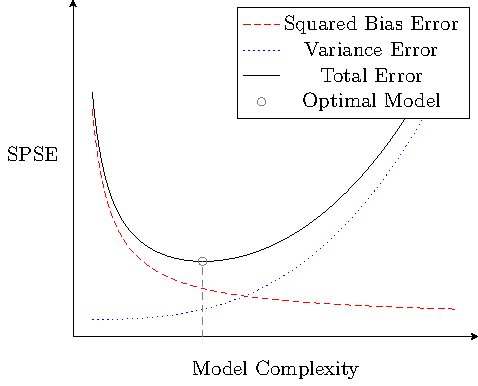
\includegraphics{graphics/pgfplots/cha2/bvd.pdf}
	\caption{Bias-variance trade-off.}
	\label{fig:bv-trade-off}
\end{figure}
%
In practice, the true value for the SPSE is not accessible since $\mu^{(i)}$ and $\sigma^2$ are unknown. Therefore, we need to estimate the SPSE. This can be done by using one of the following two strategies:

\begin{enumerate}

	\item \emph{Estimate SPSE using new and independent data} \\	
	If new observations are available, the SPSE can be estimated by
	\begin{align}
		\widehat{\text{SPSE}} = \sum_{i=1}^n \left(y^{(n+i)} - \hat y^{(i)}_M\right)^2.
	\end{align}
	These new observations can also be some held-out validation data from a train-validation split of the given data. 
	
	\item \emph{Estimate SPSE using existing data} \\
	When using existing data, the estimate for the SPSE is given by the squared error and an additional  term depending on the estimated variance and the model complexity. The estimate is thus given by
	\begin{align}
		\widehat{\text{SPSE}} = \sum_{i=1}^n \left(y^{(i)} - \hat y^{(i)}_M\right)^2 + 2\vert M \vert \hat \sigma^2.
	\end{align}

\end{enumerate}

Typically used model assessment criteria follow the basic idea of the SPSE, see \cite{fahrmeir2007regression}.

\subsubsection{Mean Squared Error} 

The mean squared error MSE is one of the standard metrics for regression and defined as

\begin{align} \label{eq:MSE-DEF}
	\mathrm{MSE} = \frac{1}{n} \sum_{i=1}^n \left(y^{(i)} - \hat y^{(i)}_M \right),	
\end{align}
%
where $y^{(i)}$ is the given data and $\hat y^{(i)}_M$ is the model prediction for that point. 

\subsubsection{Corrected Coefficient of Determination $R_{\mathrm{corr}}^2$}

The corrected coefficient of determination $R^2_{\mathrm{corr}}$ is an improvement over the coefficient of determination $R^2$, which is defined as 

\begin{align}
	R^2 = 1 - \frac{\sum_{i=1}^n \left( y^{(i)} - \hat y^{(i)}_M \right)^2}{\sum_{i=1}^n \left(y^{(i)} - \bar y\right)^2},
\end{align}
%
where $\bar y$ is the mean value of $\vec{y}$. The major drawback of $R^2$ is that it will never decrease when further inputs are included in the model, e.g. the $R^2$ of a model using $\{x_1, x_2, x_3\}$ is always larger or equal the $R^2$ of a model using $\{x_1, x_2\}$, even if the variable does not enhance the prediction quality. 

The corrected coefficient of determination $R_{\mathrm{corr}}^2$ reduces this problem by an correction term depending on the  number of parameters and is given by
\begin{align}
	R_{\mathrm{corr}}^2 = 1 - \frac{n-1}{n-p}(1-R^2).
\end{align}

The corrected coefficient of determination is a standard output parameter in many statistical programs and may be used to compare even models with different number of used variables \cite{fahrmeir2007regression}.

\subsubsection{Corrected Coefficient of Determination after McFadden $R_{\mathrm{McFadden}}^2$}

The corrected coefficient of determination after McFadden is defined as

\begin{align}
	R_{\mathrm{McFadden}}^2 = 1 - \frac{\ln{(\mathcal{L}_M)} - \vert M \vert }{\ln{(\mathcal{L}_0)}}
\end{align}
%
using the likelihood of the model $M$ given by $\mathcal{L}_M$ and the likelihood of the zero model $\mathcal{L}_0$. A standard zero model is given by the mean value $\bar y$. Higher values of $R_{\mathrm{McFadden}}^2$ correspond to better fits.

\subsubsection{Mallow's $\mathbf{C_p}$}

Mallow's complexity parameter is based directly on the ideas specified for the estimation of the SPSE and is given by

\begin{align}
	\text C_\mathrm{p} = \frac{\sum_{i=1}^n \left(y^{(i)} - \hat y^{(i)}_M\right)^2}{\hat \sigma^2} - n + 2 \vert M \vert.
\end{align}
%
A lower value of Mallow's $\text C_\mathrm{p}$ corresponds to a better model fit \cite{fahrmeir2007regression}.

\subsubsection{Akaike Information Criterion}

The AIC is among the most used model assessment criteria and defined by

\begin{align}
	\text{AIC} = -2 l(\hat{\vec{\beta}}_{\mathrm{ML}}, \hat \sigma^2_{\mathrm{ML}}) + 2(\vert M \vert +1),
\end{align}
%
where $l(\hat{\vec{\beta}}_{\mathrm{ML}}, \hat \sigma^2_{\mathrm{ML}})$ is the value of the log-likelihood~\pref{eq:log_liklihood} at its maximum, i.e. at $\hat{\vec{\beta}}_{\mathrm{ML}}$ and $\hat{\sigma}_{\mathrm{ML}}$. It is worth noting that the total number of parameters is $\vert M \vert + 1$ because the variance is also counted as parameter. The log-likelihood for a linear model assuming Gaussian errors is given by, cf.~\pref{eq:log_liklihood},

\begin{align}
	-2l(\hat{\vec{\beta}}_{\mathrm{ML}}, \hat \sigma_{\mathrm{ML}}^2) = n \log(\hat \sigma_{\mathrm{ML}}^2) + n.
\end{align}
%
Therefore, neglecting the constant $n$, the AIC evaluates to

\begin{align}
	\text{AIC} = n \log(\hat \sigma^2_{\mathrm{ML}}) + 2(\vert M \vert + 1).
\end{align}
%
A lower value of the AIC corresponds a to a better model fit \cite{fahrmeir2007regression}.

\subsubsection{Bayesian Information Criteria}

The BIC is similar to the AIC, but it penalizes more complex models much harder than the AIC. In its general form, it is given as 

\begin{align}
	\text{BIC} = -2l(\hat{\vec{\beta}}_{\mathrm{ML}}, \hat \sigma^2_{\mathrm{ML}}) + \log(n) (\vert M \vert + 1).
\end{align}
%
Again, assuming Gaussian errors for a linear model and neglecting the constant term $n$, the BIC evaluates to

\begin{align}
	\text{BIC} = n\log(\hat \sigma_{\mathrm{ML}}^2) + \log(n)(\vert M\vert + 1).
\end{align}
%
A lower value of the BIC correspond to a better model fit \cite{fahrmeir2007regression}.

\subsubsection{Cross-validation} \label{subsubsec:Cross-validation}

The basic idea of cross-validation (CV) is to split the given data set into a training set to estimate the parameters and a validation set to assess the prediction quality. A special case of cross-validation is the "leave-one-out" cross-validation, where all but one data point are used for training and the model is then evaluated on this held-out data point. This seems to be quite expensive, since one needs to estimate one model per data point. However, it can be shown that the cross-validation score can be computed using one model trained on all data $\vec{y}$ and the hat matrix $\vec{H}_M = \vec{X}_M (\transpose{\vec{X}}_M \vec{X}_M)^{-1} \transpose{\vec{X}}_M$, see Section~\pref{subsec:Hat-Matrix}. The cross-validation score is then given by

\begin{align} \label{eq:cross-validation}
	\text{CV} = \frac{1}{n} \sum_{i=1}^n \left( \frac{y^{(i)} - \hat y^{(i)}_M}{1 - h_{ii,M}} \right)^2,
\end{align}
%
where $h_{ii,M}$ denote the diagonal elements of the hat matrix $\vec{H}_M$ and $\hat y^{(i)}_M$ is defined as the prediction of the model $M$ for the input $\{x^{(i)}_1, \dots, x^{(i)}_q \}$. A lower cross-validation score corresponds to a better model fit \cite{golub1979}.

An approximation to the cross-validation score is given by the so-called generalized cross-validation (GCV) score. It is mainly used in the context of non-parametric regression, when the hat matrix $\vec{H}_M$ is numerically expensive to compute or when regularization, see Section~\pref{subsec:Regularization}, is applied. In the GCV score, the diagonal elements of the hat matrix $h_{ii,M}$ are replaced by the mean of the trace of $\vec{H}_M$. The GCV score is then given by

\begin{align} \label{eq:generalizied-cross-validation}
	\text{GCV} = \frac{1}{n}\sum_{i=1}^n \left( \frac{y^{(i)} - \hat y^{(i)}_M}{1 - \text{trace}(\vec{H}_M)/n}\right)^2.
\end{align}
%
The numerical advantage comes from the fact that the trace of a product of matrices is invariant to cyclical permutations, i.e.

\begin{align}\label{eq:trace-hat-matrix-cyclical-perm}
	\begin{split}
	\text{trace}(\vec{H}_M) {}&= \text{trace}\left(\vec{X}_M(\transpose{\vec{X}}_M \vec{X}_M)^{-1} \transpose{\vec{X}}_M\right) \\ {}&=\text{trace}\left(\transpose{\vec{X}}_M \vec{X}_M (\transpose{\vec{X}}_M \vec{X}_M)^{-1}\right) = \vert M \vert.
\end{split}
\end{align} 
%
The trace can therefore be computed from the product of two matrices of shape $\vert M \vert\times \vert M \vert$, see  \cite{fahrmeir2007regression}. Note that for a linear model as in~\pref{eq:LinearModel}, the trace of the hat matrix $\vec{H}$ is equal to the number of parameters $p$ of the linear model. For regularized or non-parametric models, the trace of the hat matrix $\vec{H}$ is smaller than $p$, where $p$ is the number of parameters of the regularized or non-parametric model. Therefore, the trace of the hat matrix $\vec{H}$ is also known as \emph{effective degree of freedom} EDoF of the model, see Section~\ref{subsec:Regularization}. 

%%%%%%%%%%%%%%%%%%%%%%%%%%%%%%%%%%%%%%%%%%%%%%%%%%%%%%%%%%%%%%%%
\subsection{Subset Selection Methods} \label{subsec:SSM}

To make use of the various model assessment criteria, some algorithmic approach to model selection needs to be given. The most commonly used approaches are forward, backward and stepwise selction \cite{fahrmeir2007regression}. 

In forward selection, we start with a candidate model, which includes a small number of variables. In each iteration of forward selection, an additional variable is added to the candidate model.  The added variable is the one which leads to the largest reduction of a predefined model assessment criteria. The algorithm stops, if no further reduction is achieved.

In backward selection, we start with a candidate model, which includes all variables. In each iteration of backward selection, we eliminate the variable from the model which elimination provides the largest improvement of a predefined model assessment criteria. The algorithm stops, if no further improvement is possible. 

In step-wise selection, forward and backward selection are combined to enable the inclusion and deletion of a variable in every operation. The algorithm stops, if no further reduction is possible.

%%%%%%%%%%%%%%%%%%%%%%%%%%%%%%%%%%%%%%%%%%%%%%%%%%%%%%%%%%%%%%%%
\subsection{Regularization} \label{subsec:Regularization}

Model selection can also be achieved using regularization techniques by directly influencing the parameters $\vec{\beta}$, which need to be estimated given a data set. In general, regularization restricts the parameter space by adding some penalty term depending on the complexity of the model to the least squares objective function according to~\pref{eq:MethodOfLS}. This leads to the penalized least squares (PLS) criterion

\begin{align} \label{eq:PLS_crit}
	\text{PLS}(\vec{y}, \vec{\beta}; \lambda) = \lVert \vec{y} - \vec{X} \vec{\beta}\rVert^2_2 + \lambda \cdot \text{pen}(\vec{\beta}),
\end{align}
%
where $\lambda$ is the so-called \emph{smoothing parameter} and $\text{pen}(\vec{\beta})$ is the penalty term describing the regularization technique. 

In Ridge regression, the penalty term in the penalized least squares criterion in~\pref{eq:PLS_crit} is given by the squared weighted $L_2$-norm of the parameter vector $\vec{\beta}$, i.e. $\text{pen}(\vec{\beta}) = \lVert \vec{\beta} \rVert^2_{\vec{K}} = \transpose{\vec{\beta}} \vec{K} \vec{\beta}$ with a positive definite penalty matrix $\vec{K} \in \mathbb{R}^{p \times p}$. The closed-form solution reads as

\begin{align}
	\hat{\vec{\beta}}_{\mathrm{PLS}} = \arg \min_{\vec{\beta}} \left(\text{PLS}(\vec{y}, \vec{\beta}; \lambda) \right) = (\transpose{\vec{X}} \vec{X} + \lambda \vec{K})^{-1} \transpose{\vec{X}}\vec{y}.
\end{align}
%
The additional penalty term in Ridge regression leads to smaller parameter estimates $\hat{\vec{\beta}}_{\mathrm{PLS}}$ compared to the unpenalized estimate $\hat{\vec{\beta}}_{\mathrm{LS}}$. For large values of the smoothing parameter $\lambda$, the parameter estimates will converge towards, but never reach, zero. 

Ridge regression is commonly used when the input dimension $q$ is high, i.e. the number of parameters $\vec{\beta}$ is large, and also known as Tikhonov regularization \cite{hoerl1970ridge}. Note that it is also possible to use a penalty matrix $\vec{K}(\vec{\beta})$ resulting in

\begin{align}
	\text{pen}(\vec{\beta}) = \lVert \vec{\beta} \rVert^2_{\vec{K}(\vec{\beta})} = \transpose{\vec{\beta}} \vec{K}(\vec{\beta}) \vec{\beta}.
\end{align}
%
However, the resulting penalized least squares problem  has no closed-form solution and must be solved by an iterative approach. We start with an initial guess $\vec{\beta}^{[0]}$ and compute for $k = 0, 1, 2, \dots$ the iteration

\begin{align} \label{eq:PLS-iterative-approach}
	\vec{\beta}^{[k+1]} = \left(\transpose{\vec{X}} \vec{X} + \lambda \vec{K}(\vec{\beta}^{[k]}) \right)^{-1} \transpose{\vec{X}} \vec{y},
\end{align}
%
until $\lVert \vec{\beta}^{[k+1]} - \vec{\beta}^{[k]} \rVert \le \text{Tol}$ with $\text{Tol}$ being a given tolerance. The derivation of the iteration~\pref{eq:PLS-iterative-approach} is presented in~\pref{apx:AppendixB}.

Note that by the introduction of the penalty matrix $\vec{K} \ne \vec{0}$, we reduce the degrees of freedom of the model. This can be seen by comparing the trace of the hat matrix $\vec{H}$ of the regularized model, i.e.

\begin{align} \label{eq:hat-matrix-regularizated-mode}
	\vec{H}_{\mathrm{pen}} = \vec{X} (\transpose{\vec{X}} \vec{X} + \lambda \vec{K})^{-1} \transpose{\vec{X}},
\end{align} 
%
with the trace of the hat matrix of the unpenalized model, see~\pref{eq:hat-matrix}. The trace of the hat matrix $\vec{H}$ is also called \emph{effective degree of freedom}, i.e.

\begin{align} \label{eq:EDoF}
	\text{EDoF} = \text{trace}(\vec{H}_{\mathrm{pen}}).
\end{align}
%
When we use regularization to reduce the degree of freedom of a model, we need to make use of the effective degree of freedom EDoF instead of the number of parameters $p$ in model assessment criteria, see Section~\pref{subsec:MAC}. 

%%%%%%%%%%%%%%%%%%%%%%%%%%%%%%%%%%%%%%%%%%%%%%%%%%%%%%%%%%%%%%%%%%%%%%%%%%%%%%%%%%%%%%%%%%%%%%%%%%%%%%%%%%%%%%%%%%
%%%%%%%%%%%%%%%%%%%%%%%%%%%%%%%%%%%%%%%%%%%%%%%%%%%%%%%%%%%%%%%%%%%%%%%%%%%%%%%%%%%%%%%%%%%%%%%%%%%%%%%%%%%%%%%%%%
\section{Splines} \label{sec:Splines}
	
A spline is a piecewise polynomial defined on a sequence of knots. This definition is quite general. Therefore, a large variety of splines exists, ranging from regression splines \cite{eubank1990regressionsplines}, over B-splines \cite{deBoor1978practicalGuideToSplines} to natural cubic splines and many more. We will focus on the definition of B-splines in Section~\pref{subsec:b-splines}, tensor-product B-splines as the multi-dimensional expansion of B-splines in Section~\pref{subsubsec:tp-splines}, and P-splines in Section~\pref{subsec:p-splines}, see for more information \cite{fahrmeir2007regression}, \cite{deBoor1978practicalGuideToSplines} and \cite{eilers1996flexible}.
%%%%%%%%%%%%%%%%%%%%%%%%%%%%%%%%%%%%%%%%%%%%%%%%%%%%%%%%%%%%%%%%%%%%%%%%%%%%%%%%%%%%%%%%%%%%%%%%%%%%%%%%%%%%%%%%%%
\subsection{B-Splines} \label{subsec:b-splines}

We put the focus on the definition and use of B-splines $s(x)$, which are constructed using the $d$ B-spline basis functions $B_j^l(x)$ of order $l$ as

\begin{align}
	s(x) = \sum_{j=1}^d B_j^l(x) \beta_j 
\end{align}
%
given the knot sequence 

\begin{align} \label{eq:knot-sequence}
	K = \left\{\kappa_{1-l}, \kappa_{1-l+1}, \dots, \kappa_{d+1}\right\}.
\end{align}
%
The B-spline basis function $B_j^l(x)$ of order $l$ is defined by means of the Cox-de Boor recursion formula as

\begin{align} \label{eq:Bspline_recDef1}
	B_j^0(x) = \begin{cases} 1 & \text{for} \quad \kappa_j \le x < \kappa_{j+1} \\ 
					 		 0 & \text{otherwise} 
	\end{cases}
\end{align}
\begin{align} \label{eq:Bspline_recDef2}
	B_j^l(x) = \frac{x - \kappa_{j-l}}{\kappa_{j} - \kappa_{j-l}} B_{j-1}^{l-1}(x) + \frac{\kappa_{j+1} - x}{\kappa_{j+1} - \kappa_{j+1-l}} B_{j}^{l-1}(x)
\end{align}
%
using the knot sequence~\pref{eq:knot-sequence}. Hence it is composed of $(l+1)$-polynomial pieces of degree $l$, see \cite{fahrmeir2007regression}. An example of a B-spline basis function of order $l=0, 1, 2, 3$ is given in~\pref{fig:spline-types-both}. 

\begin{figure}[H]
	\centering
	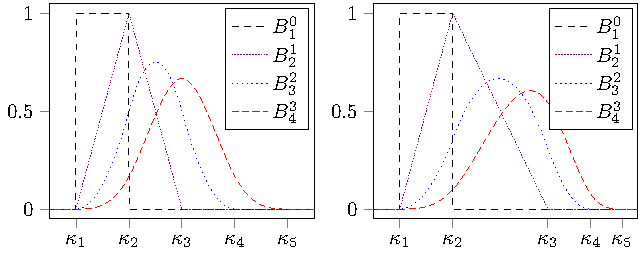
\includegraphics{graphics/pgfplots/cha2/spline-types.pdf}
	\caption{B-spline basis function of order $l=0, 1, 2, 3$ given by the superscript $l$ in $B_j^l$ for equidistant (left) and non-equidistant (right) knots.}
	\label{fig:spline-types-both}
\end{figure}

The left plot shows the B-spline basis functions based on an equidistant sequence of knots. The B-spline basis function $B_1^0$ is the zero function, except for $x \in [\kappa_1, \kappa_2]$ where it is equal to 1, see~\pref{eq:Bspline_recDef1}. The B-spline basis function $B_2^1$ is the well known \emph{hat function}, being zero except for $x \in [\kappa_1, \kappa_3]$. It consists of two linear pieces, one defined from $\kappa_1$ to $\kappa_2$, the other from $\kappa_2$ to $\kappa_3$. This can be seen by expanding the recursive definition~\pref{eq:Bspline_recDef2} to

\begin{subequations} \label{eq:Bspline-BF_21}
	\begin{align}
		B_2^1(x) = a_1(x) B_1^0(x) + a_2(x) B_2^0(x)
	\end{align}
	with
	\begin{equation}
		a_1(x) = \frac{x - \kappa_1}{\kappa_2 - \kappa_1} 
	\end{equation}
	\begin{equation}
		a_2(x) = \frac{\kappa_3 - x}{\kappa_3 - \kappa_2}. 
	\end{equation}
\end{subequations}
%
Everywhere else, $B_2^1$ is equal to zero. At the joining points, the values of the linear pieces are equal. The B-spline basis function $B_3^2$ consists of three quadratic pieces, joining at the knots $\kappa_2$ and $\kappa_3$. Expanding the recursive definition shows this as

\begin{subequations}
	\begin{align}
		B_3^2(x) = a_1(x) B_1^0(x) + a_2(x) B_2^0(x) + a_3(x) B_3^0(x)
	\end{align}
	with
	\begin{equation}
		a_1(x) = \frac{x-\kappa_1}{\kappa_3 - \kappa_1} \frac{x - \kappa_1}{\kappa_2 - \kappa_1}
	\end{equation}
	\begin{equation}
		a_2(x) = \frac{x - \kappa_1}{\kappa_3 - \kappa_1} \frac{\kappa_3 - x}{\kappa_3 - \kappa_2} + \frac{\kappa_4 - x}{\kappa_4 - \kappa_2} \frac{x - \kappa_2}{\kappa_3 - \kappa_2}
	\end{equation}
	\begin{equation}
		a_3(x) = \frac{\kappa_4 - x}{\kappa_4 - \kappa_2} \frac{\kappa_4 - x}{\kappa_4 - \kappa_3}.	
	\end{equation}
\end{subequations}
%
At $\kappa_2$ and $\kappa_3$, the values of the quadratic pieces, as well as their first-order derivatives are equal. Finally, the B-spline basis function $B_4^3$ consists of 4 cubic pieces with the joining points at $\kappa_2$, $\kappa_3$ and $\kappa_4$ at which respective cubic polynomials possess equal values as well as equal first-order and second-order derivatives. Expanding the recursive definition shows this as

\begin{subequations}
	\begin{align}
		B_4^3(x) = a_1(x) B_1^0(x) + a_2(x) B_2^0(x) + a_3(x) B_3^0(x) + a_4(x) B_4^0(x)
	\end{align}
	with 
	\begin{equation}
		a_1(x) = \frac{x - \kappa_1}{\kappa_4 - \kappa_1} \frac{x - \kappa_1}{\kappa_3 - \kappa_1} \frac{x - \kappa_1}{\kappa_2 - \kappa_1}
	\end{equation}
	\begin{equation}
		a_2(x) = \frac{x - \kappa_1}{\kappa_4 - \kappa_1} \frac{x - \kappa_1}{\kappa_3 - \kappa_1} \frac{\kappa_3 - x}{\kappa_3 - \kappa_2} + \frac{x - \kappa_1}{\kappa_4 - \kappa_1} \frac{\kappa_4 - x}{\kappa_4 - \kappa_2} \frac{x - \kappa_2}{\kappa_3 - \kappa_2} + \frac{\kappa_5 - x}{\kappa_5 - \kappa_2} \frac{x - \kappa_2}{\kappa_4 - \kappa_2} \frac{x - \kappa_2}{\kappa_4 - \kappa_2}
	\end{equation}
	\begin{equation}
		a_3(x) = \frac{x - \kappa_1}{\kappa_4 - \kappa_1} \frac{\kappa_4 - x}{\kappa_4 - \kappa_2} \frac{\kappa_4 - x}{\kappa_4 - \kappa_3} + \frac{\kappa_5 - x}{\kappa_5 - \kappa_2} \frac{x - \kappa_2}{\kappa_4 - \kappa_2} \frac{\kappa_4 - x}{\kappa_4 - \kappa_3} + \frac{\kappa_5 - x}{\kappa_5 - \kappa_2} \frac{\kappa_5 - x}{\kappa_5 - \kappa_3} \frac{x - \kappa_3}{\kappa_4 - \kappa_3}
	\end{equation}
	\begin{equation}
		a_4(x) = \frac{\kappa_5 - x}{\kappa_5 - \kappa_2} \frac{\kappa_5 - x}{\kappa_5 - \kappa_3} \frac{\kappa_5 - x}{\kappa_5 - \kappa_4}.
	\end{equation}
\end{subequations}
%
The right plot in~\pref{fig:spline-types-both} shows the B-spline basis functions of the same order $l=0,1,2,3$ defined on a non-equidistant knot sequence. The shown locality, i.e. being nonzero only over a sequence of $l+2$ knots, is a very attractive feature leading to enhanced numerical properties compared to other types of splines. Some general properties of a B-spline basis function of order $l$ are summarized in the following list. Note that these properties are valid independent of the type of the knot placement.

\begin{enumerate}[(i)]
	\item A B-spline basis function consists of $l+1$ polynomial pieces of degree $l$, e.g. a cubic B-spline basis function ($l=3$) consists of 4 cubic pieces.
	\item The pieces join at $l$ inner knots.
	\item At these knots, the derivatives up to order $l-1$ are continuous.
	\item The B-spline basis function is positive on the domain spanned by $l+2$ knots, everywhere else it is zero, e.g. for $l=2$, a sequence of 4 knots is necessary.
	\item At every given $x$, only $l+1$ B-spline basis functions are nonzero.
\end{enumerate}

Using the definition of B-spline basis functions, see~\pref{eq:Bspline_recDef1} and~\pref{eq:Bspline_recDef2}, the first-order derivative of a B-spline basis function of order $l$ is given by

\begin{align} \label{eq:Bspline-bf-derivative}
	\frac{\partial}{\partial x} B_j^l(x) = l \left[\frac{1}{\kappa_j - \kappa_{j-l}} B_{j-1}^{l-1}(x) - \frac{1}{\kappa_{j+1} - \kappa_{j+1-l}} B_j^{l-1}(x) \right]
\end{align}
%
using B-spline basis functions of order $l-1$, see \cite{fahrmeir2007regression}. Higher-order derivatives are obtained by using lower order B-spline basis functions, see \cite{deBoor1978practicalGuideToSplines}. \\

As shown in~\pref{fig:spline-types-both}, the knots can either be an equidistant sequence, which facilitates the construction and estimation of the coefficients, or a non-equidistant sequence. For equidistant knots, we split the domain $[a,b]$ into $m-1$ intervals, i.e.

\begin{align} \label{eq:equidistant-knots-interval}
	h = \frac{b - a} {m - 1},
\end{align}
%
where $m$ is given by $m = d - l + 1$ and obtain the sequence

\begin{align} \label{eq:equidistant-knots-sequence}
	\kappa_j = a + h(j-1), \quad j=1, \dots, m.
\end{align} 
%
Non-equidistant knot placement can be obtained using e.g. quantile-based knots, i.e. by using the $(j-1)/(m-1)$-quantiles for $j=1, \dots, m$ of the observed inputs $x^{(1)}, \dots, x^{(n)}$ as knots. Using this approach, more knots are placed in the areas where lots of data are present. The boundary knots, i.e. $\{\kappa_{1-l}, \dots, \kappa_0\}$ on the left side and $\{\kappa_{d-l+2}, \dots, \kappa_{d+1}\}$ on the right side, are usually set to be apart from each other by at least the minimal knot distance \cite{fahrmeir2007regression}. \\

The collection of $d$ B-spline basis functions of order $l$ over a sequence of knots $K = \{\kappa_{1-l}, \kappa_{1-l+1}, \\ \dots, \kappa_{d+1}\}$ is called B-spline basis. The basis is created such that it covers the domain $[a, b]$, i.e.

\begin{align}
	\sum_{j=1}^d B_j^l(x) = 1 \ \text{for} \ x \in [a,b].
\end{align}
%
A function $f(x)$ can then be represented with a B-spline basis by 

\begin{align} \label{eq:bspline-bf-approach}
	f(x) = \sum_{j=1}^d B_j^l(x) \beta_j = \transpose{\vec{b}} \vec{\beta}_b,
\end{align}
%
using the B-spline basis functions $B_j^l(x)$ of appropriate order $l$ and the parameter vector $\transpose{\vec{\beta}}_b = [\beta_1, \dots, \beta_d] \in \mathbb{R}^{1 \times d}$. The basis functions can be given in vector notation as $\transpose{\vec{b}} = [B_1^l(x), \dots, B_d^l(x)] \in \mathbb{R}^{1 \times d}$. Using the data set $\mathcal{D} = \{(x^{(i)}, y^{(i)}), \ i=1,2, \dots, n \}$, the B-spline basis matrix for $d$ basis functions of order $l$ is given by the matrix $\vec{B}$ as

\begin{align} \label{eq:bspline-basis-matrix}
	\vec{B} = \begin{bmatrix}
				B_1^l(x^{(1)}) & \dots & B_d^l(x^{(1)})  \\
				\vdots         &       & \vdots 		 \\
				B_1^l(x^{(n)}) & \dots & B_d^l(x^{(n)})  \\
	\end{bmatrix} \in \mathbb{R}^{n \times d}.
\end{align}
%
The $n$ equations~\pref{eq:bspline-bf-approach} can then be arranged as a linear model in the form, cf.~\pref{eq:LinearModel},

\begin{align} \label{eq:Bspline-linModel}
	\vec{y} = \vec{B} \vec{\beta}_b + \vec{\epsilon}.
\end{align}
%
Once the basis matrix in~\pref{eq:bspline-basis-matrix} is given, the parameters $\vec{\beta}_b$ can be estimated using the Least Squares algorithm given in Section~\pref{subsubsec:Method-of-LS} by minimizing the objective function

\begin{align} \label{eq:Bspline-OF}
	\text{LS}(\vec{y}, \vec{\beta}_b) = \lVert \vec{y} - \vec{B} \vec{\beta}_b \rVert_2^2.	
\end{align}
%
Therefore, the estimation is computationally efficient and easy to implement since closed-form solutions exists. Further, the advanced theoretical framework of linear models can be applied to use model selection and regularization approaches as well as to calculate e.g. confidence intervals for the parameters and the prediction.

The derivative of the function $f(x)$ in~\pref{eq:bspline-bf-approach} can be calculated by summing over all $d$ B-spline basis functions and including the estimated parameters $\vec{\beta}_b$ into the B-spline basis function derivative~\pref{eq:Bspline-bf-derivative} as

\begin{align} \label{eq:Bspline-derivative}
	\frac{\partial{f(x)}}{\partial x}= \frac{\partial}{\partial x} \sum_{j}^d B_j^l(x) \beta_j = l \sum_{j}^d \frac{\beta_j - \beta_{j-1}}{\kappa_j - \kappa_{j-l}} B_{j-1}^{l-1}(x).
\end{align}
%
\begin{comment}
The second-order derivative of $f(x)$ can be given as

\begin{align} \label{eq:Bspline-2nd-derivative}
	\frac{\partial^2 {f(x)}}{\partial{x^2}}= \frac{\partial^2}{\partial{x^2}} \sum_{j=1}^d B_j^l(x) \beta_j = l^2 \sum_{j=3}^d \frac{\Delta^2 \beta_j}{(\kappa_j-\kappa_{j-l})(\kappa_{j+1} - \kappa_{j+1-l})} B_{j-2}^{l-2}(x).
\end{align}

\begin{align} \label{eq:Bspline-2nd-derivative}
	\frac{\partial^2 {f(x)}}{\partial{x^2}}= \frac{\partial^2}{\partial{x^2}} \sum_{j=1}^d B_j^l(x) \beta_j = l^2 \sum_{j=3}^d \left[\frac{\Delta \beta_j}{(\kappa_j-\kappa_{j-l})} - \frac{\Delta \beta_{j-1}}{(\kappa_{j+1} - \kappa_{j+1-l})} \right] B_{j-2}^{l-2}(x).
\end{align}
%

Here, the finite difference operators $\Delta \beta_j = \beta_j - \beta_{j-1}$ and $\Delta^2  \beta_j = \Delta(\Delta \beta_j) = \beta_j - 2\beta_{j-1} +\beta_{j-2}$ are used. 
\end{comment}
Therefore, by estimating the B-spline parameters $\vec{\beta}_b$, we also generate an estimate for the derivative of the function $f(x)$, see \cite{fahrmeir2007regression}.

B-splines of appropriate order $l > 2$ produce smooths curves, i.e. first- and second-order derivatives are continuous, where the smoothness is mostly determined by the number of basis functions $d$ used. By using a low number $d$, the curve will be quite smooth, but possess a large data error. When using a high number of basis functions $d$, the data error will be small but the variance of the curve will be large. This is an example of the bias-variance trade-off, a classical problem of regression and supervised learning, see Section~\pref{subsubsec:SPSE} and \cite{deBoor1978practicalGuideToSplines}.  

%%%%%%%%%%%%%%%%%%%%%%%%%%%%%%%%%%%%%%%%%%%%%%%%%%%%%%%%%%%%%%%%%%%%%%%%%%%%%%%%%%%%%%%%%%%%%%%%%%%%%%%%%%%%%%%%%%

\subsubsection{Tensor-Product B-Splines} \label{subsubsec:tp-splines}

Tensor-product B-splines can be regarded as the multi-dimensional extension of B-splines. We examine an example for two input dimensions $x_1$ and $x_2$. Note that tensor-product B-splines can be constructed for arbitrary dimensions using the approach given below. The tensor-product B-spline basis function is constructed by considering the product of two B-spline basis functions of orders $l_1$ and $l_2$ of respective dimension, i.e.

\begin{align}
	T_{j,r}(x_1, x_2) = B_j^{l_1}(x_1) B_r^{l_2}(x_2)
\end{align}
%
for $j \in \{1, \dots, d_1\}$ and $r \in \{1, \dots, d_2\}$. For readability, we omit the order of the tensor-product B-spline basis function since, in principle, B-spline basis functions of arbitrary, even different orders $l_1 \ne l_2$ can be combined. We then obtain the basis function representation of the tensor-product B-spline $t(x_1, x_2)$ by summing all tensor-product B-spline basis functions as

\begin{align} \label{eq:tps-basis-function-notation}
	t(x_1,x_2) = \sum_{j=1}^{d_1} \sum_{r=1}^{d_2} T_{j,r}(x_1, x_2) \beta_{j,r} 
\end{align}
%
and in vector notation we obtain

\begin{align}
	t(x_1, x_2) = \transpose{\vec{t}} \vec{\beta}_t,
\end{align}
%
with $\transpose{\vec{t}} = [T_{1,1}(x_1, x_2), \dots, T_{d_1,1}(x_1, x_2), \dots, T_{1,d_2}(x_1, x_2), \dots, T_{d_1,d_2}(x_1, x_2)] \in \mathbb{R}^{1 \times d_1d_2}$ and the corresponding vector of parameters $\transpose{\vec{\beta}}_t = [\beta_{1,1}, \dots, \beta_{d_1,1}, \dots, \beta_{1,d_2}, \dots, \beta_{d_1, d_2}] \in \mathbb{R}^{1 \times d_1d_2}$. For any set of data 

\begin{align} \label{eq:data-2d}
	\mathcal{D} = \{ (x^{(i)}_{1}, x^{(i)}_{2}, y^{(i)} ), \ i=1,2, \dots, n\}, 
\end{align}
%
the tensor-product B-spline basis matrix for $d_1$ and $d_2$ basis functions in the respective dimensions is given by the matrix $\vec{T}$ as

\begin{align} \label{eq:tp-bspline-basis-matrix}
	\vec{T} = \begin{bmatrix}
		T_{1,1}(x_1^{(1)}, x_2^{(1)}) & \dots & T_{d_1,d_2}(x_1^{(1)}, x_2^{(1)})  \\
		\vdots         &       & \vdots 		 \\
		T_{1,1}(x_1^{(n)}, x_2^{(n)}) & \dots & T_{d_1,d_2}(x_1^{(n)}, x_2^{(n)})  \\
	\end{bmatrix} \in \mathbb{R}^{n \times d_1d_2}.
\end{align}
%	
The relationship between the tensor-product B-spline basis matrix $\vec{T}$ and the B-spline basis matrices $\vec{B}_1$ and $\vec{B}_2$ is then given as

\begin{align}
	\vec{T} = \vec{B}_2 \odot \vec{B}_1,
\end{align}
%
where $\odot$ indicates the use of the row-wise Kronecker product, see~\pref{apx:AppendixKroneckerRowWise}, $\vec{T} \in \mathbb{R}^{n \times d_1 d_2}$ denotes the tensor-product B-spline basis matrix, $\vec{B}_1 \in \mathbb{R}^{n \times d_1}$ is the B-spline basis matrix for dimension $x_1$ and $\vec{B}_2 \in \mathbb{R}^{n \times d_2}$ denotes the B-spline basis matrix for dimension $x_2$ \cite{fahrmeir2007regression}.  

We can now model a two dimensional function using the data set $\mathcal{D}$ in~\pref{eq:data-2d} similar to~\pref{eq:Bspline-linModel} as linear model of the form

\begin{align} \label{eq:tps-matrix-notation}
	\vec{y} = \vec{T} \vec{\beta}_t + \vec{\epsilon},
\end{align}
%
with the tensor-product B-spline basis matrix $\vec{T} \in \mathbb{R}^{n \times d_1 d_2}$ according to~\pref{eq:tp-bspline-basis-matrix} and the parameter vector $\transpose{\vec{\beta}}_t \in \mathbb{R}^{1 \times d_1 d_2}$. Once the basis matrix in~\pref{eq:tp-bspline-basis-matrix} is given, the parameters $\vec{\beta}_t$ can be estimated using the Least Squares algorithm given in Section~\pref{subsubsec:Method-of-LS} by minimizing the objective function 

\begin{align}
	\text{LS}(\vec{y}, \vec{\beta}_t) = \lVert \vec{y} - \vec{T} \vec{\beta}_t \rVert_2^2.
\end{align}
%
This approach can in theory be repeated for as many input dimensions as required. In practice, modeling more than two input dimensions using tensor-product B-splines becomes infeasible because of the exponential increase of basis functions and therefore parameters to estimate. 


\subsubsection{Additive Regression} \label{subsubsec:STAR}

To circumvent the latter problem, we now assume the restrictive structure of additive models, see \cite{fahrmeir2007regression}, given by

\begin{align} \label{eq:addRegBaseEquation}
	f(x_1, \dots, x_q) = f_1(x_1) + \dots + f_q(x_q).
\end{align}
%
Hence, we use one function $f_i(x_i)$ per input dimension $x_i$. For some given data set $\mathcal{D} = \{ (x^{(ii)}_{1}, \dots, x^{(ii)}_{q}, y^{(ii)} ), \ ii=1,2, \dots, n\}$, by using a B-spline for each function $f_i(x_i)$ we obtain a linear model

\begin{align} \label{eq:addRegBaseEquation-as-linModel}
	f_i(\vec{x}_i) = \vec{B}_i \vec{\beta}_{b_i},
\end{align}
%
where $\vec{B}_i \in \mathbb R^{n \times d_i}$ is the B-spline basis matrix using $d_i$ B-spline basis functions for $i=1,2,\dots, q$, $\transpose{\vec{x}}_i = [x_i^{(1)}, \dots, x_i^{(n)}] \in \mathbb{R}^{1 \times n}$ is the data vector of input dimension $i$ and $\vec{\beta}_{b_i} \in \mathbb R^{d_i}$ are the parameters to estimate. This leads to the model structure 

\begin{align} 
	\vec{y} =  \vec{B}_1 \vec{\beta}_{b_1} + \dots + \vec{B}_q \vec{\beta}_{b_q} + \vec{\epsilon},
\end{align}
%
which can be written as linear model by concatenation of the B-spline basis matrices and parameter vectors as 

\begin{align} \label{eq:STAR-single-block-diag}
	\vec{y} = \vec{X} \vec{\beta} + \vec{\epsilon}= 
				\begin{bmatrix}
					\vec{B}_1, \dots, \vec{B}_q 
				\end{bmatrix}
			    \begin{bmatrix}
					\vec{\beta}_{b_1} \\ 
					\vdots \\
					\vec{\beta}_{b_q} 
				\end{bmatrix} + \vec{\epsilon},
\end{align}
%
with the matrix $\vec{X} \in \mathbb{R}^{n \times d_{total}}$, the parameter vector $\vec{\beta} \in \mathbb{R}^{d_{total}}$ and $d_{total} = \sum_{i=1}^q d_i$ as the total number of parameters. The model~\pref{eq:STAR-single-block-diag} does not contain interaction terms between inputs. Nevertheless, these can be easily introduced for two dimensions using tensor-product B-splines without an overflowing increase in the number of coefficients. We can then write the additive model with interaction terms as 

\begin{align} \label{eq:addRegBaseEquation-with-interaction}
	f(x_1, \dots, x_q) = f_1(x_1) + \dots + f_q(x_q) + f_{1,2}(x_1, x_2) + \dots + f_{q-1, q}(x_{q-1},x_q).
\end{align}
%
Hence, we use one function $f_i(x_i)$ per input dimension and per interaction term. Using a tensor-product B-spline $t_{j,r}(x_j, x_r)$ for each interaction term, we obtain the model

\begin{align} \label{eq:STAR}
	\vec{y} = \vec{B}_1 \vec{\beta}_{b_1} + \dots + \vec{B}_q \vec{\beta}_{b_q} + \sum_{j=1}^{q-1} \sum_{r>j}^{q} \vec{T}_{j, r} \vec{\beta}_{t_{j, r}} + \vec{\epsilon},
\end{align}
%
using the tensor-product B-spline basis matrices $\vec{T}_{j,r} \in \mathbb{R}^{n \times d_j d_r}$ and the parameter $\vec{\beta}_{t_{j, r}} \in \mathbb{R}^{d_j d_r}$. Using the notation in~\pref{eq:STAR}, the theoretical framework of linear models can be applied to the additive regression model, since~\pref{eq:STAR} can be formulated as linear model yielding

\begin{align} \label{eq:STAR-block-diag}
	\vec{y} = \vec{X} \vec{\beta} + \vec{\epsilon} = 
	\begin{bmatrix}
		\vec{B}_1 , \dots , \vec{B}_q, \vec{T}_{1,2}, \dots, \vec{T}_{q-1, q}    
	\end{bmatrix} \begin{bmatrix} \vec{\beta}_{b_1} \\ 
								  \vdots \\ 
								  \vec{\beta}_{b_q} \\ 
								  \vec{\beta}_{t_{1,2}} \\ 
								  \vdots \\ 
								  \vec{\beta}_{t_{q-1, q}} \\
	\end{bmatrix} + \vec{\epsilon},
\end{align}
%
with $\vec{X} \in \mathbb{R}^{n \times d_{total}}$ as design matrix, $\vec{\beta} \in \mathbb{R}^{d_{total}}$ as parameter vector and $d_{total} = \sum_{i=1}^q d_i + \sum_{j=1}^{q-1} \sum_{r>j}^q d_j d_r$ as the total number of parameters in the model. Hence, the parameters can be calculated efficiently using the Least Squares (LS) algorithm, see Section~\pref{subsubsec:Method-of-LS}. Further, the assumptions given in~\pref{sec:LinModel} on the error term, as well as on the model function are used.

Note that additive models are not limited to be used with B-splines. We can also include the linear model given in~\pref{sec:LinModel}. For 2 input dimensions $x_1$ and $x_2$, we then obtain a model of the form

\begin{align}
	\vec{y} = \vec{X} \vec{\beta} + \vec{B}_1 \vec{\beta}_{b_1} + \vec{B}_2 \vec{\beta}_{b_2} + \vec{T}_{1,2} \vec{\beta}_{t_{1,2}},
\end{align}
%
where $\vec{X} \in \mathbb{R}^{n \times 2}$ is the design matrix of the linear model, $\vec{B}_1$ and $\vec{B}_2$ are the respective B-spline basis matrices and $\vec{T}_{1,2}$ is the tensor-product B-spline matrix. 

%%%%%%%%%%%%%%%%%%%%%%%%%%%%%%%%%%%%%%%%%%%%%%%%%%%%%%%%%%%%%%%%%%%%%%%%%%%%%%%%%%%%%%%%%%%%%%%%%%%%%%%%%%%%%%%%%%
\subsection{P-Splines} \label{subsec:p-splines}

P-splines combine the concepts of B-spline basis functions and regularization to produce sufficiently smooth function estimations. A function is said to be smooth if its second-order derivative is continuous. Therefore, a penalty of the form 

\begin{align} \label{eq:wiggliness-penalty}
	\lambda \cdot \int \left(f''(x)\right)^2 \,\mathrm{d}x
\end{align}
%
is typically introduced to penalize the curvature of a function which is measured by its second-order derivative \cite{osullivan1986penalties}. The penalty is weighted by the so-called \emph{smoothing parameter} $\lambda$. This yields the penalized least squares objective function, cf. Section~\pref{subsec:Regularization}, as

\begin{align} \label{eq:P-splines-OF-base}
	\text{PLS}(\vec{y}, \vec{\beta}; \lambda) = \lVert \vec{y} - \vec{B} \vec{\beta}_b \rVert_2^2 + \lambda \int \left(f''(x)\right)^2 \,\mathrm{d}x
\end{align}
%
using the B-spline basis matrix $\vec{B} \in \mathbb{R}^{n \times d}$ for some data $\mathcal{D}=\{(x^{(i)}, y^{(i)}), \ i=1,2,\dots,n\}$. Inserting the B-spline basis function formulation~\pref{eq:bspline-bf-approach}, using order $l$ and $d$ basis functions, into~\pref{eq:wiggliness-penalty} results in

\begin{align} \label{eq:p-spline-approx-deriv}
	\begin{split}
		\int \left(f''(x)\right)^2 \,\mathrm{d}x &= \int \left(\sum_{j=1}^d B''_j(x) \beta_j \right)^2 \,\mathrm{d}x \\
						     &= \int \sum_{j=1}^d \sum_{r=1}^d \beta_j \beta_r B''_j(x) B''_r(x) \,\mathrm{d}x \\
						     &= \transpose{\vec{\beta}} \vec{K} \vec{\beta},
	\end{split}
\end{align}
% 
with the penalty matrix $\vec{K}[j,r] = \int B''_j(x) B''_r(x) \,\mathrm{d}x$ as a matrix of dimension $\mathbb{R}^{d \times d}$. The entries of $\vec{K}$ are given by the integrated products of the second-order derivatives of the B-spline basis functions $B_j(x)$ and $B_r(x)$. For readability, the order $l$ is omitted. These second-order derivatives can be obtained by using the derivative properties of B-spline basis functions, see \cite{fahrmeir2007regression}. 

Eilers and Marx proposed in \cite{eilers1996flexible} to base the penalty on finite differences of higher order of the parameters of adjacent B-spline basis functions which circumvents the direct calculation of the second-order derivative and the integral. Hence, the complexity is reduced from $n$, the number of data points to evaluate the integral on, to $d$, the number of parameters \cite{eilers1996flexible}. The squared second-order finite difference gives a good discrete approximation of the integral of the squared second-order derivative in~\pref{eq:wiggliness-penalty}, i.e.

\begin{align} \label{eq:wiggliness-finite-diff-approx}
	\sum_{j=3}^d \left(\Delta^2 \beta_j\right)^2 \propto \int \left(f''(x)\right)^2 \,\mathrm{d}x
\end{align}
%
where $\Delta^2 \beta_j$ is defined as 

\begin{align} \label{eq:2nd-order-finite-diff}
	\begin{split}
		\Delta^2 \beta_j &= \Delta(\Delta \beta_j) \\
						 &= \Delta( \beta_j - \beta_{j-1}) \\
						 &= \beta_j - 2\beta_{j-1} + \beta_{j-2}.
	\end{split}
\end{align}
%
In matrix form,~\pref{eq:2nd-order-finite-diff} may be given as

\begin{align} \label{eq:2nd-order-finite-diff-matrix}
	\vec{D}_2 \vec{\beta}_b = 
					\begin{bmatrix} 
						1& -2      & 1&      \\  
						 &  \ddots & \ddots  & \ddots \\ 
						 &         &   1     & -2 & 1 
					\end{bmatrix} \begin{bmatrix}
						\beta_1 \\
						\vdots \\
						\beta_d
				\end{bmatrix},
\end{align}
%
with $\vec{D}_2 \in \mathbb{R}^{(d-2) \times d}$. Applying the matrix form of the second-order finite difference operator~\pref{eq:2nd-order-finite-diff-matrix} into~\pref{eq:wiggliness-finite-diff-approx} yields

\begin{align}
	\lambda \sum_{j=3}^d \left(\Delta^2 \beta_j \right)^2 = \lambda \transpose{\vec{\beta}}_b \transpose{\vec{D}}_2 \vec{D}_2 \vec{\beta}_b = \lambda \transpose{\vec{\beta}}_b \vec{K} \vec{\beta}_b.
\end{align}
%
We then obtain the objective function to minimize as

\begin{align} \label{eq:P-spline-final-OF}
	\text{PLS}(\vec{y}, \vec{\beta}; \lambda) = \lVert \vec{y} - \vec{B} \vec{\beta}_b \rVert_2^2 + \lambda \transpose{\vec{\beta}}_b \vec{K} \vec{\beta}_b,
\end{align}
%
which is equivalent to the objective function of Ridge regression, cf. Section~\pref{subsec:Regularization}, for the special choice of $\vec{K}$ given by $\vec{K} = \transpose{\vec{D}}_2 \vec{D}_2 \in \mathbb{R}^{d \times d}$. As in Ridge regression, the smoothness parameter $\lambda$ plays a critical role. For $\lambda \rightarrow 0$, the P-spline approaches the underlying B-spline since the penalty term in~\pref{eq:P-spline-final-OF} goes to $0$. For $\lambda \rightarrow \infty$, the P-spline approaches a polynomial model. The order of the polynomial is given by the order of the finite difference penalty, e.g. for second-order finite difference penalty, we penalize the discrete approximation of the second-order derivative leading to a linear function, because for these, the second-order derivative is equal to zero. Note that higher-order difference penalties are also possible.

The main advantage of P-splines is their easy set up by replacing the integral of the squared second-order derivative of the B-spline basis functions with the squared second-order finite differences of parameters of adjacent B-spline basis functions. This reduces the computational complexity and allows faster training and evaluation. Hence, P-splines are widely used in practice \cite{eilers1996flexible}. \\

A similar penalty term for tensor-product B-splines can be constructed using the Kronecker product.  Recall the definition of a tensor-product B-spline given in~\pref{eq:tps-basis-function-notation} and~\pref{eq:tps-matrix-notation}.


The spatial alignment of the B-spline basis functions and the corresponding parameters of the two-dimensional tensor-product B-spline needs to be incorporated by the definition of the term \emph{adjacent parameters}. An example for these adjacent parameters, also called spatial neighborhood, is taken from \cite{fahrmeir2007regression} and given in~\pref{fig:tps-neighborhood}. Here, we choose the parameters left and right, i.e. $\beta_{j, r-1}$ and $\beta_{j, r+1}$, as well as above and below, i.e. $\beta_{j-1,r}$ and $\beta_{j+1, r}$, as spatial neighborhood for $\beta_{j,r}$. 

\begin{figure}[H]
	\centering	
	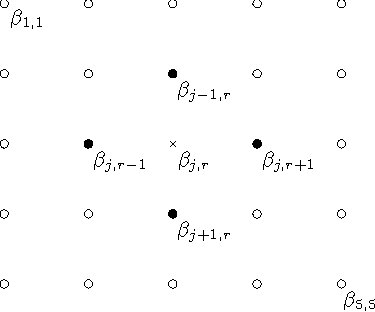
\includegraphics{graphics/pgfplots/cha2/tps-spatial-neighborhood.pdf}
	\caption{Spatial neighborhood or adjacent parameters for a tensor-product B-spline.}
	\label{fig:tps-neighborhood}
\end{figure}
%
We now use the concepts of P-splines in both dimensions and penalize the integral of the squared Hessian of the tensor-product B-spline, see~\pref{eq:wiggliness-penalty}, by a higher-order finite difference approximation in both dimensions. Using second-order finite differences as in~\pref{eq:wiggliness-finite-diff-approx} leads to the following definition of the penalty term

\begin{align}
	\left[ \sum_{j=3}^{d_1} \sum_{r=1}^{d_2} (\Delta_1^2 \beta_{j,r})^2 + \sum_{j=1}^{d_1} \sum_{r=3}^{d_2} (\Delta_2^2 \beta_{j,r})^2 \right] \propto \iint \left(f''(x_1, x_2) \right)^2 \,\mathrm{d}x_1 \,\mathrm{d}x_2
\end{align}
%
as discrete approximation of the integral of the squared Hessian of the tensor-product B-spline. The first term on the left side calculates the "row-wise" squared second-order differences, i.e. in direction $x_1$, using

\begin{align} \label{eq:row-wise-diff-operator}
	\Delta_1^2 \beta_{j,r} = \beta_{j,r} - 2\beta_{j-1,r} + \beta_{j-2,r} 
\end{align}
%
and the second term on the left side calculates the "column-wise" squared second-order differences, i.e. in direction $x_2$, using

\begin{align} \label{eq:col-wise-diff-operator}
	\Delta_2^2 \beta_{j,r} = \beta_{j,r} -2\beta_{j,r-1} + \beta_{j,r-2}.
\end{align}
%
The subscript for $\Delta$ in~\pref{eq:row-wise-diff-operator} and~\pref{eq:col-wise-diff-operator} indicates the direction of the finite differences. Using the matrix form of the second-order finite difference operator and the Kronecker product, see~\pref{apx:AppendixKronecker}, as well as the parameter vector $\vec{\beta}_t \in \mathbb{R}^{d_1 d_2 \times 1}$, we can then write the "row-wise" penalty as

\begin{align} \label{eq:row-wise-penalty}
	\transpose{\vec{\beta}}_t \transpose{(\vec{I}_{d_2} \otimes \vec{D}_{1,2})} (\vec{I}_{d_2} \otimes \vec{D}_{1,2}) \vec{\beta}_t = \sum_{j=3}^{d_1} \sum_{r=1}^{d_2} \left(\Delta_1^2 \beta_{j,r} \right)^2
\end{align}
%
and the "column-wise" penalty as

\begin{align} \label{eq:col-wise-penalty}
	\transpose{\vec{\beta}}_t \transpose{(\vec{D}_{2,2} \otimes \vec{I}_{d_1})} (\vec{D}_{2,2} \otimes \vec{I}_{d_1}) \vec{\beta}_t = \sum_{j=1}^{d_1} \sum_{r=3}^{d_2} \left(\Delta_2^2 \beta_{j,r} \right)^2
\end{align}
%
using the identity matrices $\vec{I}_{d_1} \in \mathbb{R}^{d_1 \times d_1}$ and $\vec{I}_{d_2} \in \mathbb{R}^{d_2 \times d_2}$ and the second-order difference matrices $\vec{D}_{1,2} \in \mathbb{R}^{(d_1 - 2) \times d_1}$ and $\vec{D}_{2,2} \in \mathbb{R}^{(d_2 - 2) \times d_2}$, cf.~\pref{eq:2nd-order-finite-diff-matrix}. The first subscript of $\vec{D}$ indicates the direction of the finite differences and the second subscript indicates the use of the second-order finite differences. Summing up both penalties leads to a formulation similar to~\pref{eq:P-spline-final-OF} given by

\begin{align} \label{eq:TP-P-spline-final-OF}
	\text{PLS}(\vec{y}, \vec{\beta}_t; \lambda) = \lVert \vec{y} - \vec{T} \vec{\beta}_t \rVert_2^2 + \lambda \transpose{\vec{\beta}}_t \vec{K} \vec{\beta}_t,
\end{align}
%
with the tensor-product B-spline basis matrix $\vec{T} \in \mathbb{R}^{n \times d_1 d_2}$, the smoothing parameter $\lambda$ and the penalty matrix $\vec{K}$ given by

\begin{align}
	\vec{K} = \left[ \transpose{(\vec{I}_{d_2} \otimes \vec{D}_{1,2})} (\vec{I}_{d_2} \otimes \vec{D}_{1,2}) + \transpose{(\vec{D}_{2,2} \otimes \vec{I}_{d_1})} (\vec{D}_{2,2} \otimes \vec{I}_{d_1}) \right] \in \mathbb{R}^{d_1 d_2 \times d_1 d_2}.
\end{align}
	%\chapter{Solution Approach} \label{cha:solution-approach}

The main goal of this thesis is the development and implementation using Matlab and Python of an algorithm to include a priori domain knowledge like monotonicity, curvature, unimodality, etc. into the data fitting process. Using  this additional information should improve the generalization capabilities of the model in situations of sparse, noisy or even partly wrong data. In this chapter, we use the theory discussed in~\pref{cha:fundamentals}, i.e. B-splines in Section~\ref{subsec:b-splines} and P-splines in Section~\ref{subsec:p-splines}, and extend it by adding a shape-constraint penalty term of the form 

\begin{align} \label{eq:constraint-penalty-term}
	\lambda_c \cdot \text{con}(\vec{\beta})
\end{align} 
%
depending on the user-defined a priori domain knowledge leading to the so-called \emph{shape-constraint P-splines} (SCP-splines). The various types of a priori domain knowledge that can be included are listed in Table~\ref{tab:constraint_overview}.

\begin{table}[H]
	\centering
	\begin{tabular}{|l|ll|l|}
		\hline
		\textbf{Constraint}& & \textbf{Description}   & \textbf{Section}     \\ \hline \toprule
		Jamming            & & $f(x^{(p)}) \approx y^{(p)}$ & \pref{subsec:JammC} \\ \hline 
		\multirow{2}{*}{Boundedness}  & lower & $f(x)\ge M$ 	  &	\pref{subsec:BoudC} \\ \cline{2-4}
		& upper & $f(x)\le M$    & \pref{subsec:BoudC} \\ \hline
		\multirow{2}{*}{Monotonicity} & increasing & $f'(x) \ge 0$ 	& \pref{subsec:MIC} \\ \cline{2-4}
		& decreasing & $f'(x) \le 0$  & \pref{subsec:MDC} \\ \hline	
		\multirow{2}{*}{Curvature}    & convex     & $f''(x)\ge 0$ 	& \pref{subsec:ConvC} \\ \cline{2-4}
		& concave    & $f''(x)\le 0$ 	& \pref{subsec:ConcC} \\ \hline
		\multirow{6}{*}{Unimodality}  & \multirow[t]{3}{*}{peak}  & $m = \arg \max_{x} f(x)$  & \pref{subsec:PeakC} \\ 
		&	                       & $f'(x) \ge 0 \quad \text{if} \ x < m$ & \\ 
		&  				       & $f'(x) \le 0 \quad \text{if} \ x > m$ & \\ \cline{2-4} 
		& \multirow[t]{3}{*}{valley}& $m = \arg \min_{x} f(x)$  & \pref{subsec:ValleyC} \\ 
		&	                       & $f'(x) \le 0 \quad \text{if} \ x < m$ & \\ 
		&  				       & $f'(x) \ge 0 \quad \text{if} \ x > m$ &  \\ \hline		\bottomrule
	\end{tabular}
	\caption{Overview of the considered constraints.}
	\label{tab:constraint_overview}
\end{table}
%
The focus of this chapter is the definition of shape-constraint P-splines, see Section~\ref{sec:SCP-splines}, which are characterized by their parameters $\vec{\beta}$ given by solving the optimization problem

\begin{align} \label{eq:OF-SCP-splines}
	\text{PLS}_{\text{SC}} (\vec{y}, \vec{\beta}_b; \lambda, \lambda_c) = \lVert \vec{y} - \vec{B} \vec{\beta}_b \rVert_2^2 + \lambda \cdot \text{pen}(\vec{\beta}_b) + \lambda_c \cdot \text{con}(\vec{\beta}_b),
\end{align}
%
where $\text{pen}(\vec{\beta}_b)$ is the smoothness penalty term for P-splines, see Section~\ref{subsec:p-splines}, and $\text{con}(\vec{\beta}_b)$ specifies the user-defined shape-constraint penalty term to incorporate a priori domain knowledge, see \cite{hofner2011monotonicity} and \cite{bollaerts2006simple}. We further extend the concept proposed in literature of shape-constraint P-splines to two dimensions and discuss shape-constraint tensor-product P-splines, see Section~\ref{sec:SCP-tp-splines}.

\section{Shape-constraint P-splines} \label{sec:SCP-splines}

In Section~\ref{subsec:p-splines}, we enforce smoothness by penalizing the second-order derivative of the underlying B-spline using finite differences of adjacent parameters over the whole input space to create the so-called P-splines. We will now utilize the same idea to create the shape-constrained penalty term $\text{con}(\vec{\beta}_b)$ in~\pref{eq:OF-SCP-splines}. We motivate the approach using the example of monotonic increasing behavior. The descriptions for the other constraints listed in~\pref{tab:constraint_overview} follow afterwards. In the following discussion, we use $d$ B-spline basis functions of order $l$ and the data set $\mathcal{D} = \{(x^{(i)}, y^{(i)}), \ i=1,2,\dots,n\}$ resulting in the B-spline basis matrix $\vec{X} \in \mathbb{R}^{n \times d}$. 

%%%%%%%%%%%%%%%%%%%%%%%%%%%%%%%%%%%%%%%%%%%%%%%%%%%%%%%%%%%%%%%%%%%%%%%%%%%%%%%%%%%%%%%%%%%%%%%%%%%%%%%%%%%%%
\subsection{Monotonic increasing constraint} \label{subsec:MIC}

A function is monotonic increasing if its first-order derivative is larger than or equal to zero for the whole input space. We therefore introduce a penalty of the form

\begin{align} \label{eq:SCP-penalty-base-form}
	\lambda_c \int \left(f(x)' \right)^2 \,\mathrm{d}x \quad \text{if} \ f'(x) < 0,
\end{align} 
%
to penalize negative first-order derivatives of the estimated function. The penalty is weighted by the \emph{constraint parameter} $\lambda_c$. Once again, we make use of the finite difference approximation, see Section~\ref{subsec:p-splines}. Now, the first-order derivative leads to a penalty of the form

\begin{align} \label{eq:SCP-penalty-matrix-form}
	\lambda_c \cdot \text{con}(\vec{\beta}_b) = \lambda_c \transpose{\vec{\beta}}_b \vec{K}_c \vec{\beta}_b,
\end{align}
% 
with the shape-constraint penalty matrix $\vec{K}_c = \transpose{\vec{D}}_1 \vec{V}_c \vec{D}_1 \in \mathbb{R}^{d \times d}$. The first-order derivative is approximated using the matrix form of the first-order finite difference operator $\Delta^1 \beta_j = \beta_j - \beta_{j-1}$ given by

\begin{align}\label{eq:FD-operator-order-1}
	\vec{D}_1 \vec{\beta}_b = 
	\begin{bmatrix}
		-1 &  1 &   \\
           & \ddots & \ddots \\
		   &        &  -1  & 1   
	\end{bmatrix} 
	\begin{bmatrix}
		\beta_1 \\
		\vdots \\
		\beta_d
	\end{bmatrix},
\end{align}
%
with the difference matrix $\vec{D}_1 \in \mathbb{R}^{(d-1) \times d}$. A weighting matrix $\vec{V}_c \in \mathbb{R}^{(d-1)\times(d-1)}$ is introduced to handle the if-condition in~\pref{eq:SCP-penalty-base-form}. It is a diagonal matrix with the diagonal elements $v_j$ defined as

\begin{align} \label{eq:weighting-matrix-inc-diagonal}
	v_{j-1}(\vec{\beta}_b) = \begin{cases}
		0, \quad \text{if} \ \Delta^1\beta_j \ge 0 \\ 
		1, \quad \text{if} \ \Delta^1\beta_j < 0
	\end{cases}	\ \text{for} \ j=2,3, \dots, d.
\end{align}
% 
Therefore, the weighting matrix $\vec{V}_c \coloneqq \vec{V}_c(\vec{\beta}_b)$ depends on the parameters $\vec{\beta}_b$ and we arrive at a formulation similar to Ridge regression with a parameter-dependent, non-linear penalty matrix $\vec{K} \coloneqq \vec{K}(\vec{\beta}_b)$, see Section~\ref{subsec:Regularization}. The objective function is finally of the form

\begin{align} \label{eq:OF-SCP-Final}
	\text{PLS}_{\mathrm{SCP}} (\vec{y}, \vec{\beta}_b; \lambda, \lambda_c) = \lVert \vec{y} - \vec{B} \vec{\beta}_b \rVert_2^2 + \lambda \transpose{\vec{\beta}}_b \vec{K} \vec{\beta}_b + \lambda_c \transpose{\vec{\beta}}_b \vec{K}_c \vec{\beta}_b.
\end{align}
%
We use the iterative approach given in Algorithm~\pref{alg:scp} to estimate the optimal parameters $\hat{\vec{\beta}}_{SC}$ under the user-defined shape constraint of monotonic increasing behavior.

\begin{algorithm}[H]
	\SetAlgoLined
	\KwResult{$\hat{\vec{\beta}}_{\mathrm{SC}}$}
	$ i \gets 1$\;
	$\hat{\vec{\beta}}_{i} \gets$ Solution from~\pref{eq:OF-SCP-splines} for $\lambda = \lambda_c = 0$\;
	$\vec{V}^0_c \gets \vec{0}$\;
	$\vec{V}^1_c \gets \vec{V}_c(\hat{\vec{\beta}}_{i})$\;

	\While{$\vec{V}_c^i \ne \vec{V}_c^{i-1}$}{
		$\hat{\vec{\beta}}_{i+1} = (\transpose{\vec{X}} \vec{X} + \lambda \transpose{\vec{D}}_2 \vec{D}_2 + \lambda_c \transpose{\vec{D}}_c \vec{V}^i_c \vec{D}_c)^{-1} \transpose{\vec{X}} \vec{y}$\;
		$\vec{V}^{i+1}_c \gets \vec{V}_c(\hat{\vec{\beta}}_{i+1})$\;	
		$i \gets i+1$\;
	}
	$\hat{\vec{\beta}}_{\mathrm{SC}} \gets \hat{\vec{\beta}}_{i}$\;
	\caption{Estimation of the shape-constraint P-spline coefficients.}
	\label{alg:scp}
\end{algorithm}
%
In Algorithm~\pref{alg:scp}, we make use of a Newton-Raphson scheme for the estimation of $\hat{\vec{\beta}}_{i+1}$. For more information, see~\pref{apx:AppendixB} and \cite{bollaerts2006simple}. The approach described above incorporates the shape-constraint as soft constraint depending on the constraint parameter $\lambda_c$ with the limits of no constraint for $\lambda_c \rightarrow 0$ and hard constraint for $\lambda_c \rightarrow \infty$. Therefore, $\lambda_c$ should be set by hand reflecting the user's confidence in  the a priori domain knowledge. To incorporate the other constraints listed in~\pref{tab:constraint_overview}, we need to specify the shape-constraint  penalty matrix $\vec{K}_c$ depending on the respective constraint, i.e. we define the constraint specific mapping matrix $\vec{D}_c$ and weighting matrix $\vec{V}_c$. 

%%%%%%%%%%%%%%%%%%%%%%%%%%%%%%%%%%%%%%%%%%%%%%%%%%%%%%%%%%%%%%%%%%%%%%%%%%%%%%%%%%%%%%%%%%%%%%%%%%%%%%%%%%%%%
\subsection{Monotonic decreasing constraint} \label{subsec:MDC}

Monotonic decreasing behavior can be introduced by penalizing positive first-order derivatives. Therefore, we use the matrix form of the first-order finite difference operator given in~\pref{eq:FD-operator-order-1} as mapping matrix $\vec{D}_1 \in \mathbb{R}^{(d-1) \times d}$ and define the diagonal elements of the weighting matrix $\vec{V}_c \in \mathbb{R}^{(d-1) \times (d-1)}$ as

\begin{align} \label{eq:weighting-matrix-dec-diagonal}
	v_{j-1}(\vec{\beta}_b) = \begin{cases}
		0, \quad \text{if} \ \Delta^1\beta_j \le 0 \\ 
		1, \quad \text{if} \ \Delta^1\beta_j > 0
	\end{cases},	\ \text{for} \ j=2,3, \dots, d.
\end{align}


%%%%%%%%%%%%%%%%%%%%%%%%%%%%%%%%%%%%%%%%%%%%%%%%%%%%%%%%%%%%%%%%%%%%%%%%%%%%%%%%%%%%%%%%%%%%%%%%%%%%%%%%%%%%%
\subsection{Convex constraint} \label{subsec:ConvC}

Convex behavior can be introduced by penalizing negative second-order derivatives. Therefore, we  use the matrix form of the second-order finite difference operator $\Delta^2 \beta_j = \beta_j - 2\beta_{j-1} + \beta_{j-2}$ given by

\begin{align} \label{eq:FD-operator-order-2}
	\vec{D}_2 \vec{\beta}_b = 
	\begin{bmatrix} 
		1& -2     & 1   \\  
		 & \ddots & \ddots  & \ddots \\ 
		 &        & 1       & -2     & 1 
	\end{bmatrix} \begin{bmatrix}
		\beta_1 \\
		\vdots \\
		\beta_d
	\end{bmatrix},
\end{align}
%
with the mapping matrix $\vec{D}_2 \in \mathbb{R}^{(d-2)\times d}$ and define the diagonal elements of the weighting matrix $\vec{V}_c \in \mathbb{R}^{(d-2) \times (d-2)}$ as

\begin{align} \label{eq:weighting-matrix-conv-diagonal}
	v_{j-2}(\vec{\beta}_b) = \begin{cases}
		0, \quad \text{if} \ \Delta^2\beta_j \ge 0 \\ 
		1, \quad \text{if} \ \Delta^2\beta_j < 0
	\end{cases}, \ \text{for} \ j=3,4, \dots, d.
\end{align}

%%%%%%%%%%%%%%%%%%%%%%%%%%%%%%%%%%%%%%%%%%%%%%%%%%%%%%%%%%%%%%%%%%%%%%%%%%%%%%%%%%%%%%%%%%%%%%%%%%%%%%%%%%%%%
\subsection{Concave constraint} \label{subsec:ConcC}

Concave behavior can be introduced by penalizing positive second-order derivatives. Therefore, we  use the matrix form of the second-order finite difference operator, see~\pref{eq:FD-operator-order-2}, as mapping matrix $\vec{D}_2 \in \mathbb{R}^{(d-2)\times d}$ and define the diagonal elements of the weighting matrix $\vec{V}_c \in \mathbb{R}^{(d-2) \times (d-2)}$ as

\begin{align} \label{eq:weighting-matrix-conc-diagonal}
	v_{j-2}(\vec{\beta}_b) = \begin{cases}
		0, \quad \text{if} \ \Delta^2\beta_j \le 0 \\ 
		1, \quad \text{if} \ \Delta^2\beta_j > 0
	\end{cases}, \ \text{for} \ j=3,4, \dots, d.
\end{align}

%%%%%%%%%%%%%%%%%%%%%%%%%%%%%%%%%%%%%%%%%%%%%%%%%%%%%%%%%%%%%%%%%%%%%%%%%%%%%%%%%%%%%%%%%%%%%%%%%%%%%%%%%%%%%
\subsection{Peak constraint} \label{subsec:PeakC}

Peak behavior can be introduced by penalizing negative first-order derivatives for the increasing part and positive first-order derivatives for the decreasing part of the function. Therefore, we use the matrix form of the first-order finite difference operator, see~\pref{eq:FD-operator-order-1}, as mapping matrix $\vec{D}_1 \in \mathbb{R}^{(d-1)\times d}$. The weighting matrix $\vec{V}_c \in \mathbb{R}^{(d-1) \times (d-1)}$ now has a special structure. First, we find the data point $x^{(\text{max})}$ corresponding to the peak value in the data by finding its data index $\mathrm{max}$, i.e. $\text{max} = \max_i y^{(i)} \ \text{for} \ i=1,2,\dots, n$. Next, we automatically identify the dominant B-spline basis function $B_p^l(x)$ around $x^{(\text{max})}$, i.e. the B-spline basis function with the maximal value at $x^{(\text{max})}$, such that

\begin{align}
	B_p^l(x^{(\text{max})}) \ge B_j^l(x^{(\text{max})}), \quad \text{for} \ j=1,2,\dots,d.
\end{align} 
%
We now use the index $p$ of the dominant B-spline basis function in the definition of the diagonal elements of the weighting matrix $\vec{V}_c \in \mathbb{R}^{(d-1) \times (d-1)}$ as 

\begin{align}\label{eq:v_peak_1}
	v_{j-1}(\vec{\beta}_b) &= \begin{cases} 
		0, \quad \text{if} \ \Delta^1\beta_j \ge 0 \\ 
		1, \quad \text{if} \ \Delta^1\beta_j  < 0
	\end{cases}, \quad \text{for} \ j=2,3,\dots,p
\end{align}
%
and 

\begin{align}\label{eq:v_peak_2}
	v_{j-1}(\vec{\beta}_b) &= \begin{cases} 
		0, \quad \text{if} \ \Delta^1\beta_j \le 0 \\ 
		1, \quad \text{if} \ \Delta^1\beta_j > 0
	\end{cases}, \quad \text{for} \ j=p+1,p+2,\dots,d.
\end{align}
%
%%%%%%%%%%%%%%%%%%%%%%%%%%%%%%%%%%%%%%%%%%%%%%%%%%%%%%%%%%%%%%%%%%%%%%%%%%%%%%%%%%%%%%%%%%%%%%%%%%%%%%%%%%%%%
\subsection{Valley constraint} \label{subsec:ValleyC}

Valley behavior can be introduced by the same approach as above by multiplying the data with $-1$ or by always doing the inverse operation. Therefore, we use the matrix form of the first-order finite difference operator, see~\pref{eq:FD-operator-order-1}, as mapping matrix $\vec{D}_1 \in \mathbb{R}^{(d-1) \times d}$ and define the diagonal elements of the weighting matrix $\vec{V}_c \in \mathbb{R}^{(d-1) \times (d-1)}$ as

\begin{align}\label{eq:v_valley_1}
	v_{j-1}(\vec{\beta}_b) &= \begin{cases} 
		0, \quad \text{if} \ \Delta^1\beta_j \le 0 \\ 
		1, \quad \text{if} \ \Delta^1\beta_j > 0
	\end{cases}, \quad \text{for} \ j=2,3,\dots,p
\end{align}
%
and 

\begin{align}\label{eq:v_valley_2}
	v_{j-1}(\vec{\beta}_b) &= \begin{cases} 
		0, \quad \text{if} \ \Delta^1\beta_j \ge 0 \\ 
		1, \quad \text{if} \ \Delta^1\beta_j < 0
	\end{cases}, \quad \text{for} \  j=p+1,p+2,\dots,d,
\end{align}
%
for $p$ being the index of the dominant B-spline basis function $B_p^l(x)$ around $x^{(\text{min})}$ with $\text{min} = \min_i y^{(i)} \ \text{for} \ i=1,2,\dots,n$ as data index of the valley value. 

%%%%%%%%%%%%%%%%%%%%%%%%%%%%%%%%%%%%%%%%%%%%%%%%%%%%%%%%%%%%%%%%%%%%%%%%%%%%%%%%%%%%%%%%%%%%%%%%%%%%%%%%%%%%%
\subsection{Jamming constraint} \label{subsec:JammC}

Jamming the function $f(x)$ by some point $p = (x^{(p)}, y^{(p)})$ means that the estimated function $f(x^{(p)}) \approx y^{(p)}$. This can be incorporated using the B-spline basis matrix $\vec{B} \in \mathbb{R}^{n \times d}$ as mapping matrix $\vec{D}_c \in \mathbb{R}^{n \times d}$ and a weighting matrix $\vec{V}_c \in \mathbb{R}^{n \times n}$ with diagonal elements $v_j$ given by

\begin{align} \label{eq:v_jamming}
	v_j(\vec{\beta}_b) = 
	\begin{cases}
		0, \quad \text{if} \ x^{(j)} \ne x^{(p)} \\
		1, \quad \text{if} \ x^{(j)} = x^{(p)} 
	\end{cases}, \text{for} \ j = 1,2,\dots,n.
\end{align} 

%%%%%%%%%%%%%%%%%%%%%%%%%%%%%%%%%%%%%%%%%%%%%%%%%%%%%%%%%%%%%%%%%%%%%%%%%%%%%%%%%%%%%%%%%%%%%%%%%%%%%%%%%%%%%
\subsection{Boundedness constraint} \label{subsec:BoudC}

The user-defined constraint for boundedness from below by, e.g. $M=0$ uses as mapping matrix $\vec{D}_c \in \mathbb{R}^{n \times d}$ the B-spline basis matrix $\vec{B} \in \mathbb{R}^{n \times k}$. For the weighting matrix $\vec{V}_c \in \mathbb{R}^{n\times n}$, the diagonal weights $v_j$ are defined as

\begin{align} \label{eq:v_boundedness}
	v_j(\vec{\beta}_b) = \begin{cases} 
		0, \quad \text{if} \ f(x^{(j)}) \ge M\\ 
		1, \quad \text{if} \ f(x^{(j)})  < M 		
	\end{cases}, \text{for} \ j=1,2,\dots,n.
\end{align}
%
Using different values of $M$ allows us to bound from below from any number $M$. Switching the comparison operators in~\pref{eq:v_boundedness} enables us to bound functions from above. 


%%%%%%%%%%%%%%%%%%%%%%%%%%%%%%%%%%%%%%%%%%%%%%%%%%%%%%%%%%%%%%%%%%%%%%%%%%%%%%%%%%%%%%%%%%%%%%%%%%%%%%%%%%%%%%%
%%%%%%%%%%%%%%%%%%%%%%%%%%%%%%%%%%%%%%%%%%%%%%%%%%%%%%%%%%%%%%%%%%%%%%%%%%%%%%%%%%%%%%%%%%%%%%%%%%%%%%%%%%%%%%%
\section{Shape-constraint tensor-product P-splines}\label{sec:SCP-tp-splines}

In  Section~\ref{subsubsec:tp-splines}, we extended the univariate approach of B-splines to bivariate tensor-product B-splines by using the row-wise Kronecker product, see~\pref{apx:AppendixKroneckerRowWise}. We will now extend the tensor-product P-splines, see Section~\ref{subsec:p-splines}, to incorporate a priori domain knowledge as in~\pref{sec:SCP-splines} into the fitting process. We start by showing how to include a priori domain knowledge in one dimension, see Section~\pref{subsec:MIC-TP-one-dim}, and describe the various constraints listed in~\pref{tab:constraint_overview_2d}. Afterwards, we show how to include a constraint based on both dimensions, see Section~\pref{subsec:MULTICON-TP-one-dim}. In the following discussion, we use $d_1$ and $d_2$ B-spline basis functions of order $l$ for the dimensions 1 and 2 respectively and the data set $D = \{(x_1^{(i)}, x_2^{(i)}, y^{(i)}), \ i=1,2,\dots,n\}$ resulting in the tensor-product B-spline basis matrix $\vec{T} \in \mathbb{R}^{d_1d_2 \times n}$.

\begin{table}[H]
	\centering
	\begin{tabular}{|l|ll|l|}
		\hline
		\textbf{Constraint}& & \textbf{Description}   & \textbf{Section}     \\ \hline \toprule
		\multirow{2}{*}{Monotonicity} & increasing & $ \frac{\partial f(x_1,x_2)}{\partial x_1} \ge 0$ 	& \pref{subsec:MIC-TP-one-dim} \\ \cline{2-4}
		& decreasing & $\frac{\partial f(x_1,x_2)}{\partial x_1} \le 0$  & \pref{subsec:MDC-TP-one-dim} \\ \hline	
		\multirow{2}{*}{Curvature}    & convex     & $\frac{\partial^2 f(x_1,x_2)}{\partial x_1^2}\ge 0$ 	& \pref{subsec:CONV-TP-one-dim} \\ \cline{2-4}
		& concave    & $\frac{\partial^2 f(x_1,x_2)}{\partial x_1^2}\le 0$ 	& \pref{subsec:CONC-TP-one-dim} \\ \hline 
		Multiple  & & & \pref{subsec:MULTICON-TP-one-dim} \\ \hline \bottomrule
	\end{tabular}
	\caption{Overview of the constraints for shape-constraint tensor-product P-splines.}
	\label{tab:constraint_overview_2d}
\end{table}

Note that the constraints \emph{Jamming} and \emph{Boundedness} in~\pref{tab:constraint_overview} are dimension-independent and therefore not listed in~\pref{tab:constraint_overview_2d}. Nevertheless, the can also be applied to tensor-product B-splines using the descriptions in Section~\ref{subsec:JammC} and~\ref{subsec:BoudC}. We will present the scheme for input dimension 1. For dimension 2, minor changes need to be done, e.g. some reordering in the weighting matrix $\vec{V}_c$. 
%%%%%%%%%%%%%%%%%%%%%%%%%%%%%%%%%%%%%%%%%%%%%%%%%%%%%%%%%%%%%%%%%%%%%%%%%%%%%%%%%%%%%%%%%%%%%%%%%%%%%%%%%%%%%%%

\subsection{Monotonic increasing constraint in dimension 1} \label{subsec:MIC-TP-one-dim}

A function is monotonic increasing in dimension 1 if its first-order derivative in dimension 1 is larger than or equal to zero for the whole input space. Therefore, we introduce a penalty of the form

\begin{align} \label{eq:SCP-tp-penalty-base-from}
	\lambda_c \iint \left( \frac{\partial f(x_1, x_2)}{\partial x_1} \right)^2 \,\mathrm{d}x_1 \,\mathrm{d}x_2 \quad \text{if} \ \frac{\partial f(x_1, x_2)}{\partial x_1} < 0,
\end{align} 
%
to penalize negative first-order partial derivatives of the estimated function. The penalty term is again weighted by the \emph{constraint parameter} $\lambda_c$. Approximating the first-order derivative by finite-differences of order 1, similar to~\pref{eq:row-wise-penalty} and~\pref{eq:col-wise-penalty}, leads to a penalty of the known form 

\begin{align} \label{eq:shape-constraint-inc-dim1}
	\lambda_c \cdot \text{con}(\vec{\beta}_t) = \lambda_c \transpose{\vec{\beta}}_t \vec{K}_c \vec{\beta}_t,
\end{align}
%
with the shape-constraint penalty matrix $\vec{K}_c = \transpose{\vec{D}}_c \vec{V}_c \vec{D}_c \in \mathbb{R}^{d_1d_2 \times d_1d_2}$. The first-order derivative is approximated by the matrix form of the first-order finite difference operator, see~\pref{eq:FD-operator-order-1}, and by using the Kronecker product, cf.~\pref{apx:AppendixKronecker}, as

\begin{align} \label{eq:mapping-matrix-sc-tp-increasing}
	\vec{D}_c \vec{\beta}_t = \big( \vec{I}_{d_2} \otimes \vec{D}_{1}\big) \vec{\beta}_t,
\end{align}
%
with the mapping matrix $\vec{D}_c \in \mathbb{R}^{(d_1-1)d_2 \times d_1d_2}$ using the identity matrix $\vec{I}_{d_2} \in \mathbb{R}^{d_2 \times d_2}$ and the finite-difference matrix for the first dimension $\vec{D}_{1} \in \mathbb{R}^{(d_1-1) \times d_1}$. The diagonal elements $v_j$ of the weighting matrix $\vec{V}_c \in \mathbb{R}^{(d_1-1)d_2 \times (d_1-1)d_2}$ are defined as

\begin{align}
	\begin{split}
	v_{j+(i-1)(d_1-1)}(\vec{\beta}_t) ={}& \begin{cases}
		0, \quad \text{if} \ \Delta^1_{d_1} \beta_{j+(i-1)d_1 + 1} \ge 0 \\ 
		1, \quad \text{if} \ \Delta^1_{d_1} \beta_{j+(i-1)d_1 + 1} < 0 
	\end{cases}, \\ {}& \text{for} \ j=1,2,\dots,d_1-1 \ \text{and} \ i=1,2,\dots,d_2,
	\end{split}
\end{align}
%
using the first-order finite-difference operator for dimension 1 $\Delta^1_{d_1}$ defined as

\begin{align} \label{eq:FD-operator-dim1}
	\Delta^1_{d_1} \beta_j = \beta_j - \beta_{j-1}.
\end{align}
%
Hence, we obtain an objective function similar to~\pref{eq:OF-SCP-splines} as

\begin{align} \label{eq:OF-SCP-tp-splines}
	\text{PLS}_{\text{SC-TP}} (\vec{y}, \vec{\beta}_t; \lambda, \lambda_c) = \lVert \vec{y} - \vec{T} \vec{\beta}_t \rVert_2^2 + \lambda \transpose{\vec{\beta}}_t \vec{K} \vec{\beta}_t + \lambda_c \transpose{\vec{\beta}}_t \vec{K}_c \vec{\beta}_t,
\end{align}
%
with the smoothness penalty matrix $\vec{K} \in \mathbb{R}^{d_1d_2 \times d_1d_2}$, see Section~\ref{subsec:p-splines}, and the shape-constraint penalty matrix $\vec{K} \in \mathbb{R}^{d_1d_2 \times d_1d_2}$. The optimal parameters under the shape constraint $\hat{\vec{\beta}}_{\text{SC-TP}}$ can be estimated using the iterative scheme given in Algorithm~\pref{alg:scp}.

%%%%%%%%%%%%%%%%%%%%%%%%%%%%%%%%%%%%%%%%%%%%%%%%%%%%%%%%%%%%%%%%%%%%%%%%%%%%%%%%%%%%%%%%%%%%%%%%%%%%%%%%%%%%%
\subsection{Monotonic decreasing constraint for dimension 1} \label{subsec:MDC-TP-one-dim}

Monotonic decreasing behavior in dimension 1 can be introduced by penalizing positive first-order partial derivatives. Therefore, we use the matrix form of the first-order finite difference operator given in~\pref{eq:FD-operator-order-1}, i.e. $\vec{D}_1 \in \mathbb{R}^{(d_1-1) \times d_1}$, in the set up of the mapping matrix $\vec{D}_c \in \mathbb{R}^{(d_1-1)d_2 \times d_1d_2}$, see~\pref{eq:mapping-matrix-sc-tp-increasing}, and define the diagonal elements of the weighting matrix $\vec{V} \in \mathbb{R}^{(d_1-1)d_2 \times (d_1-1)d_2}$ as

\begin{align} 
	\begin{split}
	v_{j+(i-1)(d_1-1)} (\vec{\beta}_t) ={}& \begin{cases}
		0, \quad \text{if} \ \Delta^1_{d_1} \beta_{j+(i-1)d_1 + 1} \le 0 \\ 
		1, \quad \text{if} \ \Delta^1_{d_1} \beta_{j+(i-1)d_1 + 1} > 0
	\end{cases},	\\ {}& \text{for} \ j=1,2,\dots,d_1-1 \ \text{and} \ i=1,2,\dots,d_2,
	\end{split}
\end{align}
%
using the first-order finite difference operator for dimension 1 in~\pref{eq:FD-operator-dim1}.

%%%%%%%%%%%%%%%%%%%%%%%%%%%%%%%%%%%%%%%%%%%%%%%%%%%%%%%%%%%%%%%%%%%%%%%%%%%%%%%%%%%%%%%%%%%%%%%%%%%%%%%%%%%%%
\subsection{Convex constraint for dimension 1} \label{subsec:CONV-TP-one-dim}

Convex behavior in dimension 1 can be introduced by penalizing negative second-order partial derivatives. Therefore, we  use the matrix form of the second-order finite difference operator in~\pref{eq:FD-operator-order-2}, i.e. $\vec{D}_2 \in \mathbb{R}^{(d_1-2) \times d_1}$, in the set up of the mapping matrix $\vec{D}_c \in \mathbb{R}^{(d_1-2)d_2 \times d_1d_2}$, see~\pref{eq:mapping-matrix-sc-tp-increasing}, and define the diagonal elements of the weighting matrix $\vec{V}_c \in \mathbb{R}^{(d_1-2)d_2 \times (d_1-2)d_2}$ as

\begin{align}
	\begin{split}
	v_{j+(i-1)(d_1-2)}(\vec{\beta}_t) {}&= \begin{cases}
		0, \quad \text{if} \ \Delta^2_{d_1} \beta_{j+(i-1)d_1+2} \ge 0 \\ 
		1, \quad \text{if} \ \Delta^2_{d_1} \beta_{j+(i-1)d_1+2} < 0
	\end{cases}	\\ {}& \text{for} \ j=1,2,\dots,d_1-2 \ \text{and} \ i=1,2,\dots,d_2,
	\end{split}
\end{align}
%
using the second-order finite difference operator for dimension 1 defined as

\begin{align} \label{eq:FD-operator2-dim1}
	\Delta^2_{d_1} \beta_j = \beta_j - 2\beta_{j-1} + \beta_{j-2}.
\end{align}

%%%%%%%%%%%%%%%%%%%%%%%%%%%%%%%%%%%%%%%%%%%%%%%%%%%%%%%%%%%%%%%%%%%%%%%%%%%%%%%%%%%%%%%%%%%%%%%%%%%%%%%%%%%%%

\subsection{Concave constraint for dimension 1} \label{subsec:CONC-TP-one-dim}

Concave behavior in dimension 1 can be introduced by penalizing positive second-order partial derivatives. Therefore, we  use the matrix form of the second-order finite difference operator in~\pref{eq:FD-operator-order-2}, i.e. $\vec{D}_2 \in \mathbb{R}^{(d_1-2) \times d_1}$, in the set up of the mapping matrix $\vec{D}_c \in \mathbb{R}^{(d_1-2)d_2 \times d_1d_2}$, see~\pref{eq:mapping-matrix-sc-tp-increasing}, and define the diagonal elements of the weighting matrix $\vec{V}_c \in \mathbb{R}^{(d_1-2)d_2 \times (d_1-2)d_2}$ as

\begin{align}
	\begin{split}
	v_{j+(i-1)(d_1-2)}(\vec{\beta}_t) {}&= \begin{cases}
		0, \quad \text{if} \ \Delta^2_{d_1} \beta_{j+(i-1)d_1+2} \le 0 \\ 
		1, \quad \text{if} \ \Delta^2_{d_1} \beta_{j+(i-1)d_1+2} > 0
	\end{cases}	\\ {}& \text{for} \ j=1,2,\dots,d_1-2 \ \text{and} \ i=1,2,\dots,d_2,
	\end{split}
\end{align}
%
using the second-order finite difference operator for dimension 1 defined in~\pref{eq:FD-operator2-dim1}.

%%%%%%%%%%%%%%%%%%%%%%%%%%%%%%%%%%%%%%%%%%%%%%%%%%%%%%%%%%%%%%%%%%%%%%%%%%%%%%%%%%%%%%%%%%%%%%%%%%%%%%%%%%%%%
\subsection{Shape constraints in two dimensions} \label{subsec:MULTICON-TP-one-dim}

To enforce shape constraints in two dimensions, e.g monotonic increasing behavior in dimension 1 ($c_1$) and monotonic decreasing behavior in dimension 2 ($c_2$), we use the same idea as given in~\pref{subsec:MIC-TP-one-dim} for both dimensions. Hence, we obtain an objective function similar to~\pref{eq:OF-SCP-splines} as

\begin{align} \label{eq:OF-SCP-tp-splines_2constraints}
	\text{PLS}_{\mathrm{SC-TP}} (\vec{y}, \vec{\beta}_t; \lambda, \lambda_{c_1}, \lambda_{c_2}) = \lVert \vec{y} - \vec{T} \vec{\beta}_t \rVert_2^2 + \lambda \transpose{\vec{\beta}}_t \vec{K} \vec{\beta}_t + \lambda_{c_1} \transpose{\vec{\beta}}_t \vec{K}_{c_1} \vec{\beta}_t + \lambda_{c_2} \transpose{\vec{\beta}}_t \vec{K}_{c_2} \vec{\beta}_t,
\end{align}
%
with the smoothness penalty matrix $\vec{K} \in \mathbb{R}^{d_1d_2 \times d_1d_2}$, see Section~\ref{subsec:p-splines}, and two \emph{constraint parameter} $\lambda_{c_1}$ and $\lambda_{c_2}$ reflecting the users trust in the a priori domain knowledge. The optimal parameters under the shape constraint $\hat{\vec{\beta}}_{\mathrm{SC-TP}}$ can then be estimated again using the iterative scheme given in Algorithm~\pref{alg:scp}.

	%\chapter{Practical Considerations}

In~\pref{cha:solution-approach}, we discussed the theoretical basis for shape-constraint P-splines and their ability to incorporate a priori domain knowledge by choice of the constraint term described by the mapping matrix $\vec{D}_c$ and the weighting matrix $\vec{V}_c$. We will now consider the practical application of these, as well as their limits in terms of data fitting and constraint holding. 

It is important to notice that the addition of the constraint term in~\pref{eq:OF-SCP-Final} further reduces the effective degree of freedom of the model, similar as for P-splines, resulting in a less flexible model. We therefore expect that the measured metric on the training data will be worse compared to a pure B-spline fit. Nevertheless, the metric of interest is the measured error on the validation data, i.e. the held out data that the model has not seen before. Supposing that the a priori domain knowledge reflects the true, underlying function, we expect the measured error on the validation data to be lower than or equal to the error given by an optimal P-spline fit. Here, optimality is based on the optimal smoothing parameter $\lambda$ given by generalized cross-validation, see Section~\ref{subsubsec:Cross-validation}. This can be seen by recognizing the equivalence of the objective functions for P-splines, see~\pref{eq:P-spline-final-OF}, and shape-constraint P-splines, see~\pref{eq:OF-SCP-Final}, when the underlying B-spline fit does not violate the user-defined constraint, i.e. all $v_j=0$. This feature is one of the limits of shape-constraint P-splines, i.e. we cannot influence the model using this approach if no constraint violations are present. On the other hand, if the a priori domain knowledge reflects the underlying function, we can expect a far better generalization capability of the model compared to the B-spline fits, especially in situations of noisy or sparse data.

In this chapter, we are going to discuss the practical incorporation of a priori domain knowledge based on the example of peak behavior, see~\pref{sec:peak-behav}. We will evaluate the performance of shape-constraint P-splines using sparse and noisy data and compare it to B-splines and P-splines. Further, we will discuss the effect of the constraint parameter $\lambda_c$, see~\pref{sec:lambda_c_sec}.

%%%%%%%%%%%%%%%%%%%%%%%%%%%%%%%%%%%%%%%%%%%%%%%%%%%%%%%%%%%%%%%%%%%%%%%%%%%%%%%%%%%%%%%%%%%%%%%%%%%%%%%%%%%%%%%%%%%%%%%%%%%%%%%%%
\section{Peak Constraint in Practice} \label{sec:peak-behav}

We will now use shape-constraint P-splines and the a priori domain knowledge of peak behavior to fit the data $D = \{(x^{(i)}, y^{(i)}), \ i=1,2,\dots,n\}$. The data is artificially generated by random sampling of $n=200$ points $x^{(i)}$ of the function $f$, i.e.

\begin{align} \label{eq:test-func-peak}
	y^{(i)} = f(x^{(i)}) + \epsilon^{(i)} = \exp\big(-\frac{(x^{(i)} - 0.35)^2}{0.1}\big) + \epsilon^{(i)} \quad \text{for} \ x^{(i)} \in [0.1,0.8],
\end{align}
%
with $\epsilon^{(i)}$ being Gaussian noise with mean $\mu = 0$ and variance $\sigma^2 = 0.01$. We randomly split the data in a training set $D_t$ with 150 samples and a validation set $D_v$ with 50 samples. At first, we use $d=45$ B-spline basis functions of order $l=3$ to fit a B-spline to the training data $D_t$. Then, we fit a P-spline using the same number of basis functions $d$ and order $l$ with an optimal smoothness parameter $\lambda_{opt} = 7.74$ chosen by generalized cross-validation. Finally, we enforce the peak behavior by using a shape-constraint P-spline using the same number of basis functions $d$ and order $l$ as well as the optimal smoothness parameter $\lambda_{opt}=3.68$ and the constraint parameter $\lambda_c=6000$ reflecting high trust in the a priori domain knowledge. The various fits are evaluated on the validation data $D_v$ and shown in~\pref{fig:test-func-peak-fit}. The mean squared errors on the validation data, as well as on the true, underlying function in~\pref{eq:test-func-peak}, are given~\pref{tab:test-func-peak-mses}.


\begin{figure}[H]
	\centering
	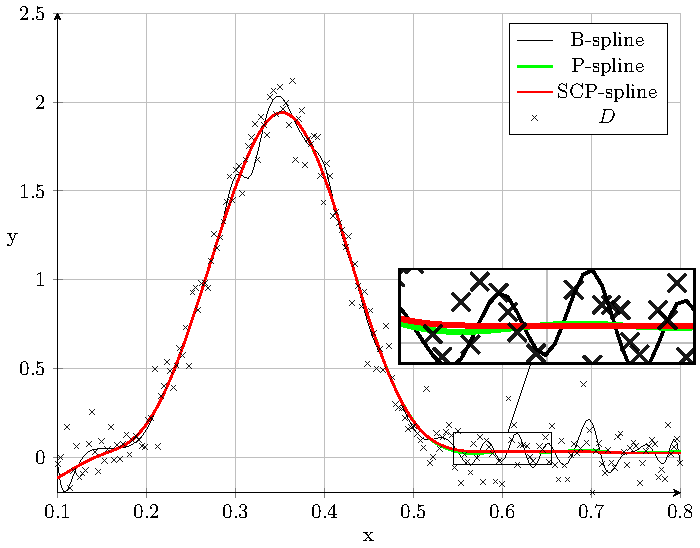
\includegraphics{graphics/pgfplots/cha4/exp-peak.pdf}
	\caption{B-spline, P-spline and SCP-spline fit for $D_v$.}
	\label{fig:test-func-peak-fit}
\end{figure}
%
The B-spline, as black curve in~\pref{fig:test-func-peak-fit}, captures the basic shape of the true function, but the flexibility of the B-spline, due to the high number of B-splines, leads to a wiggly curve especially for the almost constant part. This violates the peak behavior of the true function, i.e. being non-increasing after the peak value. For the P-spline, as green curve, this problem relaxes due to the smoothing aspect of the penalty term but does not vanish, as seen in the magnified part in~\pref{fig:test-func-peak-fit1}. Note that the additional smoothness penalty given by the P-spline already fits the data almost perfectly. The SCP-spline fit adjusts only the parts of the P-spline, which violate the constraint. It may be seen as "fine-tuning" of the fit using the a priori domain knowledge. Hence, it is the best solution here as it is nearly constant for the necessary parts of the function in~\pref{eq:test-func-peak}.  

\begin{table}[H]
	\begin{center}
		\pgfplotstabletypeset[
		col sep=comma,
		columns/Model/.style={string type},
		columns/MSEVal/.style={column name={$\text{MSE}_{D_v}$}},
		columns/MSEValTrueFunction/.style={column name={$\text{MSE}_{D_{v,true}}$}},
		every head row/.style={before row=\toprule[1pt] \toprule,after row=\midrule[2pt]},
		every last row/.style={after row=\bottomrule \bottomrule},
		every nth row={1}{before row=\midrule},
		]{graphics/data/cha4/peak_example/mse.csv}
	\end{center}
	\caption{Mean squared errors on the validation set.}
	\label{tab:test-func-peak-mses}
\end{table}
%
The mean square errors on the noisy validation data $D_v$ in~\pref{tab:test-func-peak-mses} for P-spline and SCP-spline are almost identical and do not show a favorable model. Comparing the various models with the true, underlying function, see $\text{MSE}_{D_{v,true}}$ in~\pref{tab:test-func-peak-mses}, leads to the assessment that the SCP-spline is the more accurate model with regards to the true function behavior. This coincides with the graphs in~\pref{fig:test-func-peak-fit}. Hence, the incorporation of a priori domain knowledge via shape-constraints improves the generalization capability measured by the mean squared error on the true function values. 
%%%%%%%%%%%%%%%%%%%%%%%%%%%%%%%%%%%%%%%%%%%%%%%%%%%%%%%%%%%%%%%%%%%%%%%%%%%%%%%%%%%%%%%%%%%%%%%%%%%%%%%%%%%%%%%%%%%%%%%%%%%%%%%%%

\section{Sparse Data and the Peak Constraint}

We will now examine the behavior of B-, P- and SCP-splines for sparse data, i.e. little data and uneven distributed, sampled from the function in~\pref{eq:test-func-peak}. The data set $D$ now contains 70 data points distributed in a way that there is little data in the peak region, i.e for $x \in [0.2, 0.5]$ we have only 10 data points. We perform an random train-validation split of the data in $D$, i.e. the training data $D_t$ consists of 52 points and the validation data $D_v$ consists of 18 points. We follow the same approach as above, i.e. fit a B-spline, perform generalized cross-validation to fit the optimal P-spline and finally apply the shape-constraint to enforce peak behavior. The small data set indicates that a different, not equidistant knot placement may be helpful. Hence, we carry out 2 experiments, one with equidistant knot placement and the other with quantile-based knot placement, see Section~\ref{subsec:b-splines}. We chose to use $d=25$ B-spline basis functions of order $l=3$. The optimal smoothness parameter was given as $\lambda_{opt} = 0.00657$ for the equidistant fit and $\lambda_{opt} = 0.00215$ for the quantile-based fit. The constraint parameter $\lambda_c$ was set to $\lambda_c=1000$ for both fits, reflecting high trust in the a priori domain knowledge. The resulting fits are shown in~\pref{fig:sparse-example-equidistant} and~\pref{fig:sparse-example-quantile}.


\begin{figure}[H]
	\centering
	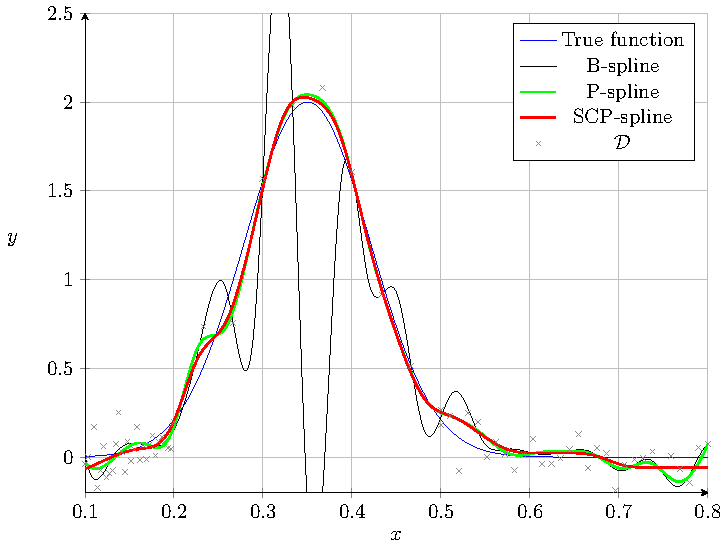
\includegraphics{graphics/pgfplots/cha4/exp-sparse-equidistant.pdf}
	\caption{Equidistant B-spline, P-spline and SCP-spline fit for sparse data $D$.}
	\label{fig:sparse-example-equidistant}
\end{figure}


\begin{figure}[H]
	\centering
	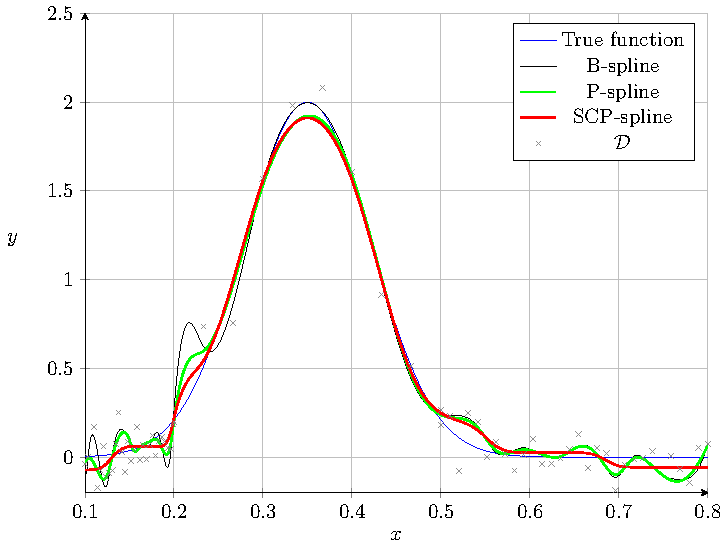
\includegraphics{graphics/pgfplots/cha4/exp-sparse-quantile.pdf}
	\caption{Quantile-based B-spline, P-spline and SCP-spline fit for sparse data $D$.}
	\label{fig:sparse-example-quantile}
\end{figure}


%%%%%%%%%%%%%%%%%%%%%%%%%%%%%%%%%%%%%%%%%%%%%%%%%%%%%%%%%%%%%%%%%%%%%%%%%%%%%%%%%%%%%%%%%%%%%%%%%%%%%%%%%%%%%%%%%%%%%%%%%%%%%%%%%

\section{Lambda c} \label{sec:lambda_c_sec}


\section{Something}
In this chapter we use the theory discussed in Chapter \pref{cha:fundamentals} to estimate uni- and bivariate  functions using data and a priori domain knowledge. An overview of the different problems considered in this chapter is given in Table \pref{tab:problem_overview}. 

\begin{table}[H]
	\centering
	\begin{tabular}{|l|l|l|l|}
		\hline
		\textbf{Univariate}   & \textbf{Section} & \textbf{Bivariate}         & \textbf{Section} \\ \hline \toprule
		B-splines             &                & Tensor-product B-splines   &               \\ \hline
		P-splines             &                & Tensor-product P-splines   &              \\ \hline
		SCP-splines           & 			   & Tensor-product SCP-splines &     \\ \hline \bottomrule
	\end{tabular}
	\caption{Problem overview.}
	\label{tab:problem_overview}
\end{table}
%
First, we are using B-splines, see Section~\pref{subsec:b-splines}, for the estimation of the unknown function $y = f(x)$, i.e. we solve the optimization problem

\begin{align} \label{eq:OF-B-splines}
	\arg \min_{\vec{\beta}} Q_1(\vec{y}, \vec{\beta}) = \lVert \vec{y} - \vec{X} \vec{\beta} \rVert,
\end{align}
%
using the B-spline or tensor-product B-spline basis matrix $\vec{X}$. Next, we use the concept of P-splines, see Section~\pref{subsec:p-splines}, to estimate smooth functions, i.e. we solve the optimization problem

\begin{align} \label{eq:OF-P-splines}
	\arg \min_{\vec{\beta}} Q_2(\vec{y}, \vec{\beta}; \lambda) = \lVert \vec{y} - \vec{X} \vec{\beta} \rVert + \lambda \cdot \text{pen}(\vec{\beta}),
\end{align}
%
where $\text{pen}(\vec{\beta})$ specifies a smoothness penalty term. Finally, we are going to incorporate a priori domain knowledge into the fitting process using shape-constrained P-splines (SCP-splines), i.e. we solve the optimization problem
\begin{align} \label{eq:OF-SCP-splines}
	\arg \min_{\vec{\beta}} Q_3(\vec{y}, \vec{\beta}; \lambda, \lambda_c) = \lVert \vec{y} - \vec{X} \vec{\beta} \rVert + \lambda \cdot \text{pen}(\vec{\beta}) + \lambda_c \cdot \text{con}(\vec{\beta}),
\end{align}
%
where $\text{pen}(\vec{\beta})$ is again a smoothness penalty term and $\text{con}({\vec{\beta}})$ specifies the user-defined shape-constraint to incorporate a priori domain knowledge with, see \cite{hofner2011monotonicity} and \cite{bollaerts2006simple}. Various types a priori domain knowledge can be incorporated using the constraints listed in~\pref{tab:constraint_overview}.



The focus of this chapter is the definition and use of shape-constraint P-splines, which are characterize by their parameters $\vec{\beta}$ given by solving the optimization problem~\pref{eq:OF-SCP-splines}.


	%\chapter{Practical Applications} \label{cha:practical-appl}

We will now apply the concept of shape-constraint P-splines at real-world data to incorporated a priori domain knowledge into the modeling process. In the first example, see~\pref{sec:real-world-application}, we use the domain knowledge to enhance the estimation of the heat transfer coefficient in a heat-treatment process. The main challenge here is the sparse and noisy data situation combined with a highly non-linear process. In the second example, see~\pref{sec:real-world-application2}, we investigate the behavior of a servo compensation which possesses a discontinuity as main challenge.  

\section{Parameter Estimation} \label{sec:real-world-application}

The data is generated from a heat-treatment process of aluminum strips. The aluminum strip is heated up to a specific temperature, hold at this temperature for some predefined time and then rapidly cooled down to room temperature by means of water jets. The controlled heating and cooling enhances the temperature evolution  and thus the specific mechanical properties of the aluminum strip. 

\begin{figure}[H]
	\centering
	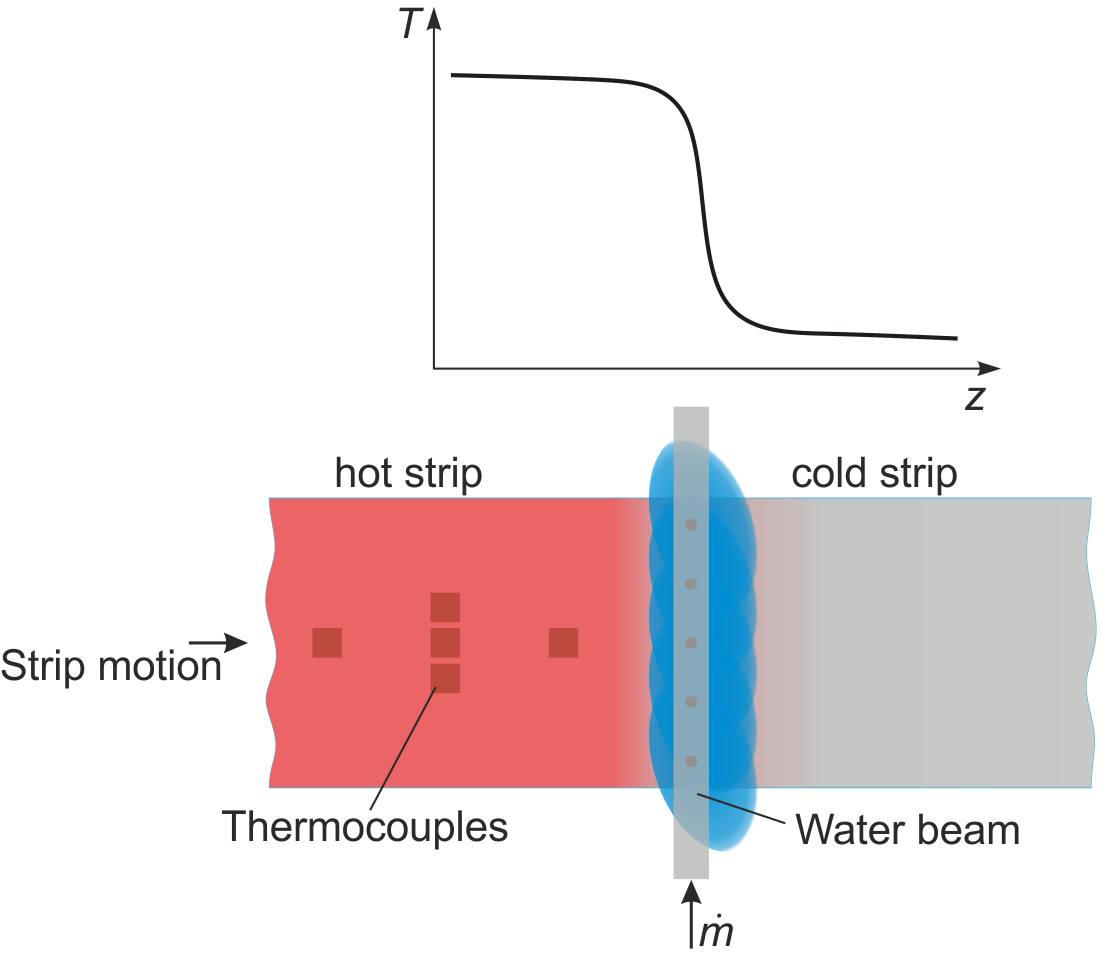
\includegraphics[width=0.8\columnwidth]{graphics/pgfplots/cha5/Ebner/Water_Beam.png}
	\caption{Schematic representation of the aluminum strip and the water beam.}
	\label{fig:ebner_water_beam}
\end{figure}

The area of interest is the cooling phase of the strip, in which some highly non-linear processes take place due to phase transitions of the cooling medium water, see~\pref{fig:ebner_water_beam}. The temperature evolution T of the strip mainly depends on the heat transfer coefficient $\alpha$ characterizing the interaction between the aluminum strip and water. A complete description of the physical effects during water cooling is still research. Therefore, modeling of the heat transfer coefficient using first-principle methods is not expedient. Nevertheless, we can use the first-principle ideas in the form of a priori domain knowledge. To describe the temperature evolution during the cooling phase, we try to estimate the heat transfer coefficient, i.e.

\begin{align}
	\alpha := \alpha(T, \dot m),
\end{align}
%
as a function of the temperature $T$ of the aluminum strip and the mass flow $\dot m$ of the cooling medium. We know beforehand, that the heat transfer coefficient $\alpha$ may only increase with increasing mass flow $\dot m$ and that it shows unimodal peak behavior for increasing temperature $T$, motivated by the so-called Nukiyama curve given in~\pref{fig:ebner_nukiyama}, see \cite{mayinger2013stromung} and \cite{baehr2006heatandmasstransfer}.
	  
\begin{figure}[H]
	\centering
	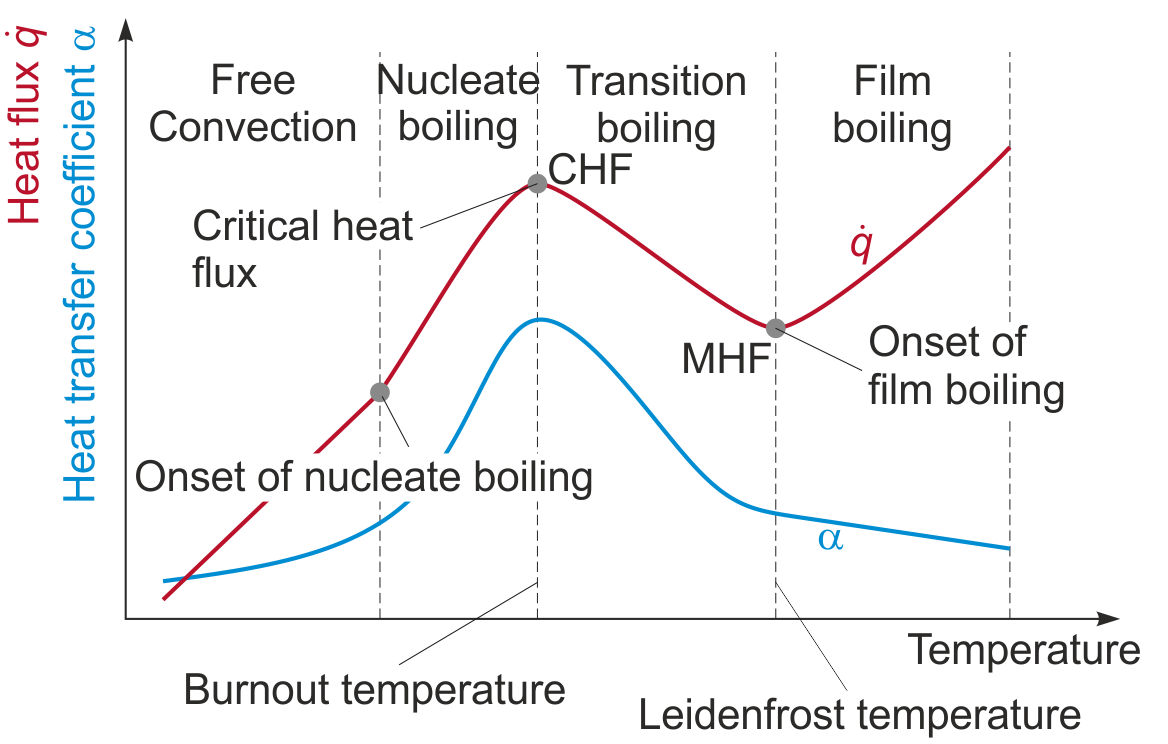
\includegraphics[width=0.8\columnwidth]{graphics/pgfplots/cha5/Ebner/Nukiyama_Curve.png}
	\caption{Nukiyama curve.}
	\label{fig:ebner_nukiyama}
\end{figure}

The data is determined by elaborate experiments performed on a prototype of Ebner Industrieofenbau. The distribution of data is visualized in~\pref{fig:ebner_data_situation}. Here we show how many data points are given in a square area of approximately 50 $\si{K}$ and 0.9 $\si{kg}/\si{s}$, which represent approximately 1\% of the whole input space. We have some regions, where no data is available, while the majority of data points is located in small areas, see~\pref{sec:peak-behav-sparse}. This problem, i.e. of irregular data distribution, is often encountered in real-world situations. 

\begin{figure}[H]
	\centering
	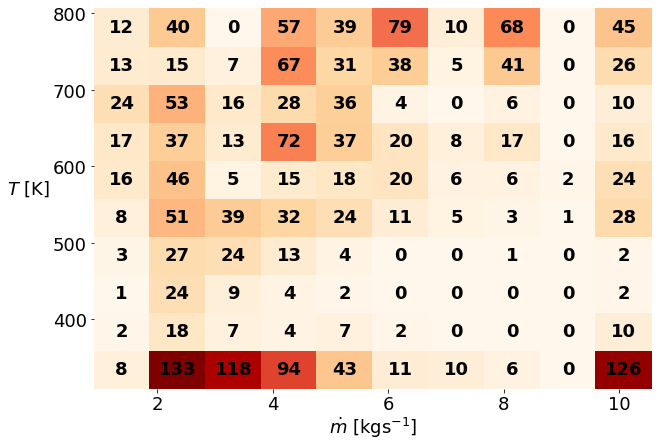
\includegraphics[width=0.8\columnwidth]{graphics/pgfplots/cha5/Ebner/data_distribution.png}
	\caption{Data distribution.}
	\label{fig:ebner_data_situation}
\end{figure}

The data distribution may lead to some difficulties when using B-splines and tensor-product B-splines, as they do not handle sparse data situations well, cf.~\pref{cha:practical-considerations}. Nevertheless, using regularization via smoothness and constraint penalties should help to cope with the data situation. 

We will now use various models based on B-spline bases, tensor-product B-spline bases and their shape-constraint alternatives to recover a model for the heat transfer coefficient given the data. The following list, in which $s(x_i)$ denotes the use of a B-spline basis for input $x_i \in \{\dot{m}, T\}$ and $t(\dot{m}, T)$ denotes the use of a tensor-product B-spline basis, describes the models that are analyzed. 

\begin{enumerate}[(i)]
	\item M1 $= s(\dot{m}) + s(T)$ without constraints
	\item M2 $= s(\dot{m}) + s(T)$, with monotonicity for $s(\dot{m})$ and unimodal peak behavior for $s(T)$
	\item M3 $= t(\dot{m}, T)$ without constraints
	\item M4 $= t(\dot{m}, T)$, with monotonicity for input $\dot{m}$
	\item M5 $= s(\dot{m}) + s(T) + t(\dot{m}, T)$, as additive model without constraints
	\item M6 $= s(\dot{m}) + s(T) + t(\dot{m}, T)$, as additive model with constraints defined in M2 and M4
\end{enumerate}
%
Note that we use a smoothness penalty optimized via generalized cross-validation for each individual basis. The unconstraint models M1, M3 and M5 are therefore P-spline models rather than pure B-spline models. The shape-constraint models M2, M4 and M6 are SCP-spline models. 


To fit the models listed above, we perform a randomized train-validation split on the data, i.e. we split the data into a training set $\mathcal{D}_{\text{train}}$ and a validation set $\mathcal{D}_{\text{val}}$, fit the models to the resulting training set and evaluate its performance by calculating the mean squared error MSE, see~\pref{eq:MSE-DEF}, on the validation set $\mathcal{D}_{\text{val}}$ and the effective degree of freedom EDoF of the model, see~\pref{eq:EDoF}, as well as by visual inspection. We choose to split the data into sets of the same size to generate a more stable estimation of the prediction error for previously unseen data. A visual inspection of the of the data distribution given by the train-validation split is given in~\pref{fig:ebner-train-val-split}.

\begin{figure}[H]
	\centering
	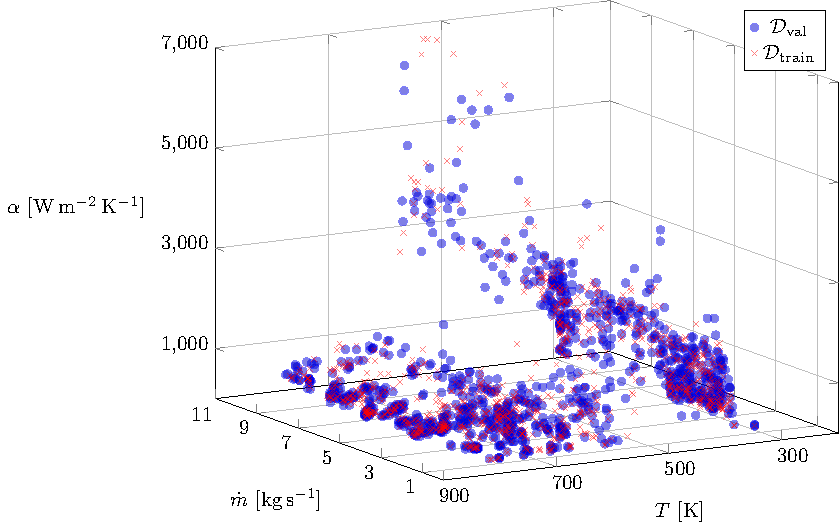
\includegraphics[width=\columnwidth]{graphics/pgfplots/cha5/Ebner/train-val-split.pdf}
	\caption{Validation set $\mathcal{D}_{\text{val}}$ and training set $\mathcal{D}_{\text{train}}$.}
	\label{fig:ebner-train-val-split}
\end{figure}
%

The mean squared errors $\mathrm{MSE}_{\mathrm{val}}$ evaluated on the validations set $\mathcal{D}_{\text{val}}$ as well as the effective degree of freedom EDoF of the models are given in~\pref{tab:ebner-mse-val}. According to these, the superior model is M4, i.e. the shape-constraint tensor-product B-spline with a monotonicity constraint in the mass flow dimension. The models M3, i.e. the tensor-product P-spline, and M6, i.e. the additive model using shape-constraints, perform nearly as well as M4 according to the mean squared error on the validation set but both possess a significantly higher EDoF which allows for some overfitting. 

\begin{table}[H]
	\begin{center}
		\pgfplotstabletypeset[
		col sep=comma,
		columns/Model/.style={string type},
		columns/MSE_val/.style={column name={$\text{MSE}_{\text{val}}$}},
		every head row/.style={before row=\toprule[1pt] \toprule,after row=\midrule[2pt]},
		every last row/.style={after row=\bottomrule \bottomrule},
		every nth row={1}{before row=\midrule},
		]{graphics/data/cha5/Ebner/mses.csv}
	\end{center}
	\caption{Mean squared errors on the validation set $\mathcal{D}_{\text{val}}$ and effective degree of freedom EDoF of the models.}
	\label{tab:ebner-mse-val}
\end{table}

The predictions for model M4 are shown in~\pref{fig:ebner-M4}. The peak behavior in the temperature dimension is clearly visible, as well as an increasing trend within the mass flow dimension. Therefore, we conclude that model M4 is the superior model with regards to the domain knowledge and data fidelity. 

\begin{figure}[H]
	\centering
	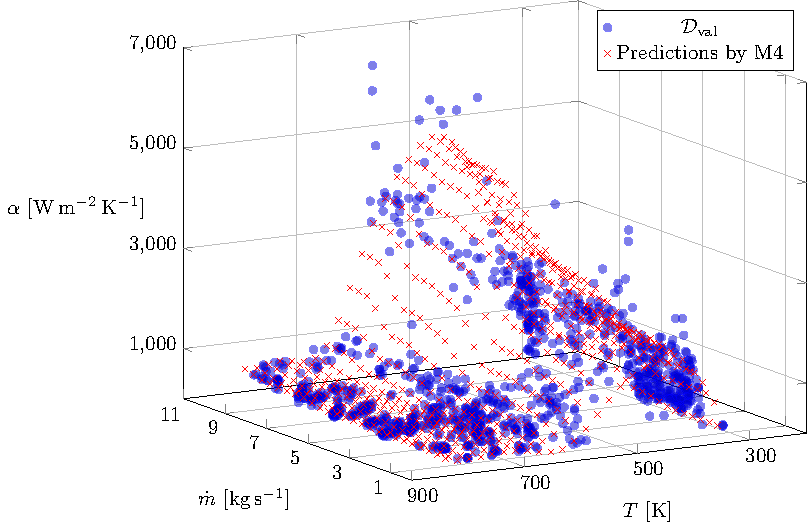
\includegraphics[width=\columnwidth]{graphics/pgfplots/cha5/Ebner/M4.pdf}
	\caption{Validation set $\mathcal{D}_{\text{val}}$ and predictions by model M4.}
	\label{fig:ebner-M4}
\end{figure}

The predictions for model M6 are shown in~\pref{fig:ebner-M6}. Here, the peak behavior can also be identified, but in a weaker fashion as for model M4 in~\pref{fig:ebner-M4}. We also obtain an increasing trend in the mass flow dimension. 

\begin{figure}[H]
	\centering
	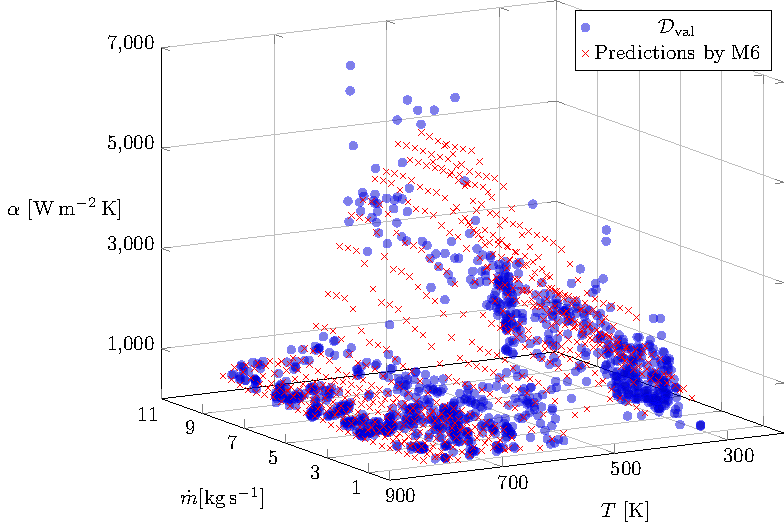
\includegraphics[width=\columnwidth]{graphics/pgfplots/cha5/Ebner/M6.pdf}
	\caption{Validation set $\mathcal{D}_{\text{val}}$ and predictions by model M6.}
	\label{fig:ebner-M6}
\end{figure}
%
The visual inspection of the predictions of model M3 in~\pref{fig:ebner-M3} indicates that there is massive overfitting present. Neither smooth, nor the a priori known behavior (increasing in the mass flow dimension and a peak behavior in the temperature dimension) is identifiable.  

\begin{figure}[H]
	\centering
	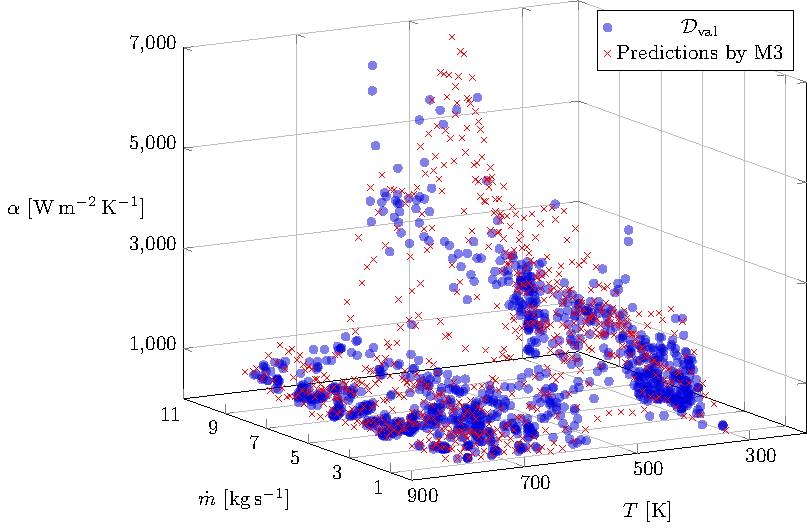
\includegraphics[width=\columnwidth]{graphics/pgfplots/cha5/Ebner/M3.pdf}
	\caption{Validation set $\mathcal{D}_{\text{val}}$ and predictions by model M3.}
	\label{fig:ebner-M3}
\end{figure}

We omit the visual presentation of the predictions by the models M1, M2 and M5, since for all of these the metrics, mean squared errors on the validation set $\mathcal{D}_{\text{val}}$ and the effective degree of freedom EDoF, indicate even worse models.

To summarized, we see that the incorporation of a priori domain knowledge improves the quality of the fit in all of the above models, e.g. M2 outperforms M1, M4 outperforms M3 and M6 outperforms M5 according to the mean squared errors on the validation set $\mathcal{D}_{\text{val}}$, respectively. Therefore, we conclude that the incorporation of a priori domain knowledge through shape-constraints improves the model quality for our real-world data example. 

%%%%%%%%%%%%%%%%%%%%%%%%%%%%%%%%%%%%%%%%%%%%%%%%%%%%%%%%%%%%%%%%%%%%%%%%%%%%%%%%%%%%%%%%%%%%%%%%%%%%%%%%%%%%%%%%%%%%%%%%%%%%%%%%%%%%%%%%%%%%%%%%%%%%%%%%%%%%%%%%%%%%%%%%%%%%%%%%%%%%%%%%%%%%%%%%%%%%%%%%%%%%%%%%%%%%%%%%%%%%%%%%%%%%%%%%%%%%%%%%
%%%%%%%%%%%%%%%%%%%%%%%%%%%%%%%%%%%%%%%%%%%%%%%%%%%%%%%%%%%%%%%%%%%%%%%%%%%%%%%%%%%%%%%%%%%%%%%%%%%%%%%%%%%%%%%%%%%%%%%%%%%%%%%%%%%%%%%%%%%%%%%%%%%%%%%%%%%%%%%%%%%%%%%%%%%%%%%%%%%%%%%%%%%%%%%%%%%%%%%%%%%%%%%%%%%%%%%%%%%%%%%%%%%%%%%%%%%%%%%%
\section{Hybrid Modeling and Control Example} \label{sec:real-world-application2}

As a second example, we consider a hybrid modeling and control concept applied to a hydraulic 4/3 two-stage directional control valve. A mathematical model and a model-based control concept was derived and validated by means of measurements on a test bench in a former project at the Austrian Institute of Technology. Since the pilot valve is of overlapping design, the system has a large dead zone. This dead zone aggravates high precision positioning and places high demands on the controller design. A reduced-order model $\Sigma$ was derived using singular perturbation techniques. It can be formulated as a Hammerstein system which consists of a linear system and a static input nonlinearity. Here, the input is given by the voltage $u$ and outputs are the main valve piston position $s_h$ and the current $i_p$, respectively. 


\begin{figure}[H]
	\centering
	\includegraphics[width=0.8\columnwidth]{graphics/pgfplots/cha5/Bosch/blockschaltbild.png}
	\caption{Block diagram of the control concept.}
	\label{fig:blockschaltbild}
\end{figure}
%
The proposed (cascaded) control concept, which is depicted in~\pref{fig:blockschaltbild}, consists of a current controller $R_i$, a compensation (marked in red) and a position controller $R_{sh}$ for the main valve piston position. The compensation is composed of a pressure observer $\hat{\Sigma}$ and a servo compensation, and can be described by a function of the form 

\begin{align} \label{eq:ex-2-equation}
	i_m^d = f(q_p^d, s_h^d),
\end{align}
%
where $s_h^d$ denotes the desired main valve piston position and $q_p^d$ is the desired differential volume flow. The function~\pref{eq:ex-2-equation} represents the most complex part (in terms of the amount of operations and the number of parameters) of the designed control concept. Therefore, we aim to replace it by a function approximation. 

The data $\mathcal{D}$ consisting of 1000 points is generated using a validated model-based on first-principles and visualized in Figure \ref{fig:bosch_data_situation}. The figure shows two distinct model regions with a discontinuity at the desired main valve piston position $s_h^d = 0 \ \si{m}$. The main challenge here is to model the discontinuity in a smooth way without introducing modeling artifacts, i.e. over- or undershooting behavior. We know beforehand that the differential current $i_m^d$ is monotonic increasing with the desired differential volume flow $q_p^d$. We further constrain the models to be monotonic increasing with the desired main valve piston position $s_h^d$ to enforce a smooth transition at the discontinuity at $s_h^d = 0 \ \si{m}$.

\begin{figure}[H]
	\centering
	\includegraphics{graphics/pgfplots/cha5/Bosch/data_situation.pdf} 
	\caption{Data Situation}
	\label{fig:bosch_data_situation}
\end{figure}

We will now use various models based on B-spline bases, tensor-product B-spline bases and their shape-constraint alternatives to recover a model for the differential current $i_m^d$. The following list, in which $s(x_i)$ denotes the use of a B-spline basis for input $x_i \in \{q_p^d, s_h^d\}$ and $t(q_p^d, s_h^d)$ denotes the use of a tensor-product B-spline basis, describes the models that are analyzed.

\begin{enumerate}[(i)]
	\item M1 $= s(q_p^d) + s(s_h^d)$, without constraints
	\item M2 $= s(q_p^d) + s(s_h^d)$, with monotonicity for $s(s_h^d)$
	\item M3 $= t(q_p^d,s_h^d)$, without constraints
	\item M4 $= t(q_p^d,s_h^d)$, with monotonicity for input $s(q_p^d)$ and $s(s_h^d)$
	\item M5 $= s(s_h^d) + t(q_p^d,s_h^d)$, as additive model without constraints
	\item M6 $= s(s_h^d) + t(q_p^d,s_h^d)$, as additive model with the constraints defined in M2 and M4
\end{enumerate}
%
Note that we use a smoothness penalty optimized via generalized cross-validation for each individual basis. The unconstraint models M1, M3 and M5 are therefore P-spline models rather than pure B-spline models. The shape-constraint models M2, M4 and M6 are SCP-spline models. 


To fit the models listed above, we perform a randomized train-validation split on the data. The training set $\mathcal{D}_{\text{train}}$ then consists of 750 data points and a validation set $\mathcal{D}_{\text{val}}$ of 250 data points. We fit the models to the resulting training set and evaluate its performance by calculating the mean squared error on the validation set $\mathcal{D}_{\text{val}}$ and the effective degree of freedom of the models EDoF, as well as by visual inspection.


The mean squared errors $\mathrm{MSE}_{\mathrm{val}}$ evaluated on the validations set $\mathcal{D}_{\text{val}}$ are given in~\pref{tab:bosch-mse-val} as well as the effective degree of freedom of the models as a measure of model complexity. 

\begin{table}[H]
	\begin{center}
		\pgfplotstabletypeset[
		col sep=comma,
		columns/Model/.style={string type},
		columns/MSE_val/.style={column name={$\text{MSE}_{\text{val}}$}},
		every head row/.style={before row=\toprule[1pt] \toprule,after row=\midrule[2pt]},
		every last row/.style={after row=\bottomrule \bottomrule},
		every nth row={1}{before row=\midrule},
		]{graphics/data/cha5/Bosch/mses.csv}
	\end{center}
	\caption{Mean squared errors on the validation set $\mathcal{D}_{\text{val}}$ and the effective degree of freedom $\text{EDoF}$ of the models.}
	\label{tab:bosch-mse-val}
\end{table}

The purely B-spline based models M1 and M2 show low degrees of freedom but higher values of the mean squared error on the validation set $\mathcal{D}_{\text{val}}$. Therefore, they lack some flexibility to model the data accurately. The predictions of these models are visualized in~\pref{fig:bosch-M1} and~\pref{fig:bosch-M2}. Note the left plot is the projection of the three dimensional data onto the $s_h^d$ axis for better visualization of the model predictions. The purely tensor-product B-spline models M3 and M4 have a significantly lower mean squared error on the validation set $\mathcal{D}_{\text{val}}$. Both models are visualized in~\pref{fig:bosch-M3} and~\pref{fig:bosch-M4}. With regards to the effective degree of freedom, we see that the regularization through the shape-constraints clearly decreases the model flexibility which leads to a better generalization behavior seen by the lower $\text{MSE}_{\text{val}}$ of M4 compared to M3. This can also be seen in the left plot of~\pref{fig:bosch-M3}. Note, for example, the prediction point (red) at $q_p^d \approx 0.7 \cdot 10^{-4} \ \si{\cubic m s^{-1}}$. Such a prediction is only possible for a very wiggly and non-smooth function. The additive models using B-splines and tensor-product B-splines, i.e. M5 and M6, both show low mean squared errors on the validation set $\text{MSE}_{\text{val}}$. We again see the effect of the shape-constraint in the effective degree of freedom as well as in the visualizations in~\pref{fig:bosch-M5} and~\pref{fig:bosch-M6}. 

\begin{figure}[H]
	\centering 
	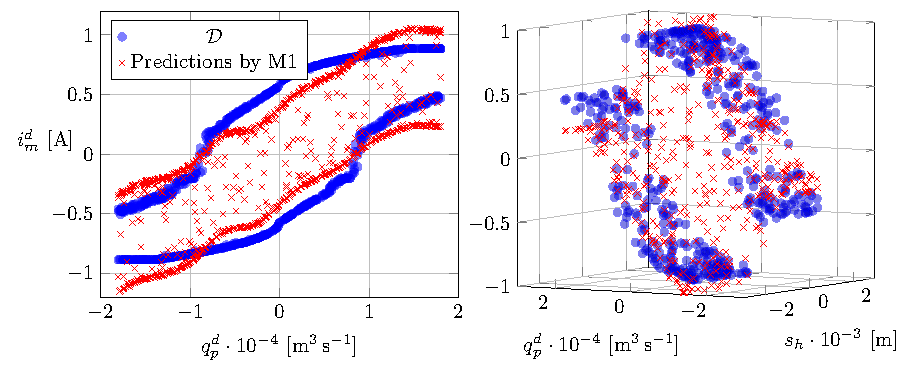
\includegraphics{graphics/pgfplots/cha5/Bosch/M1.pdf}
	\caption{Data $\mathcal{D}$ and predictions by model M1.}
	\label{fig:bosch-M1}
\end{figure}

\begin{figure}[H]
	\centering 
	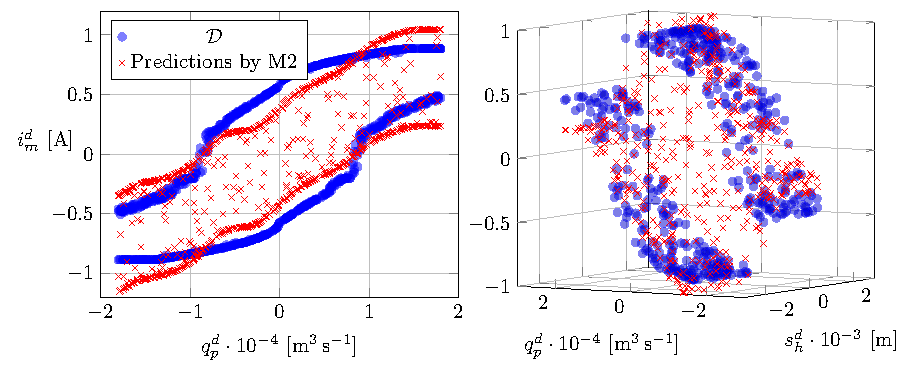
\includegraphics{graphics/pgfplots/cha5/Bosch/M2.pdf}
	\caption{Data $\mathcal{D}$ and predictions by model M2.}
	\label{fig:bosch-M2}
\end{figure}

\begin{figure}[H]
	\centering 
	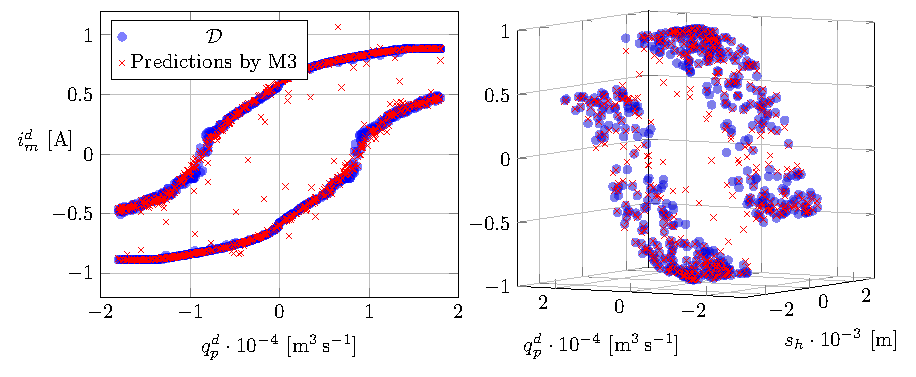
\includegraphics{graphics/pgfplots/cha5/Bosch/M3.pdf}
	\caption{Data $\mathcal{D}$ and predictions by model M3.}
	\label{fig:bosch-M3}
\end{figure}

\begin{figure}[H]
	\centering 
	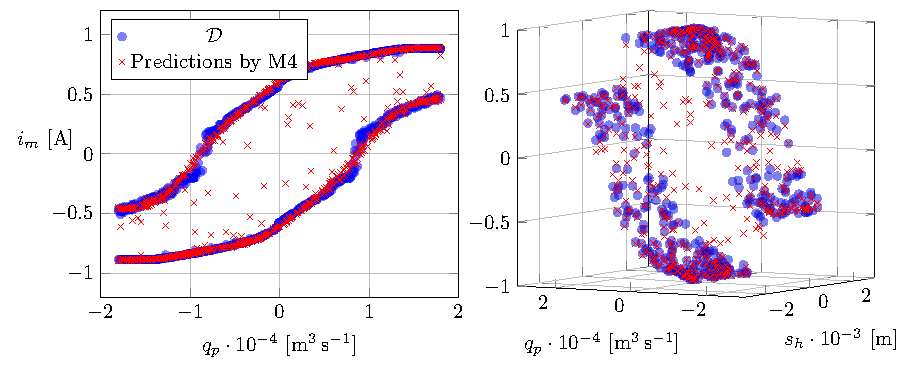
\includegraphics{graphics/pgfplots/cha5/Bosch/M4.pdf}
	\caption{Data $\mathcal{D}$ and predictions by model M4.}
	\label{fig:bosch-M4}
\end{figure}

\begin{figure}[H]
	\centering 
	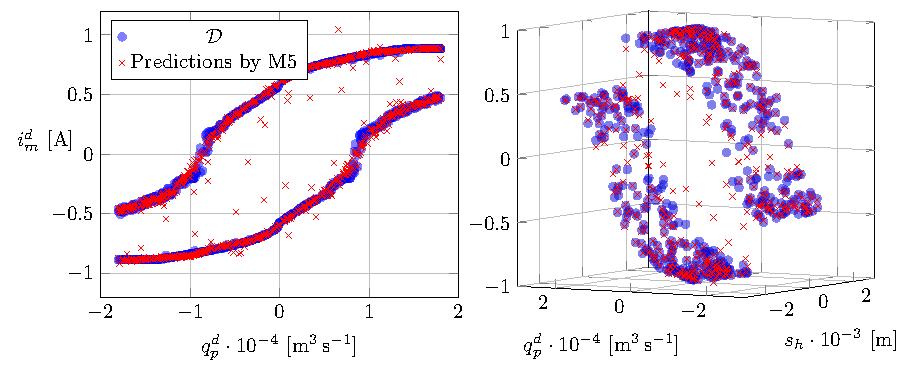
\includegraphics{graphics/pgfplots/cha5/Bosch/M5.pdf}
	\caption{Data $\mathcal{D}$ and predictions by model M5.}
	\label{fig:bosch-M5}
\end{figure}

\begin{figure}[H]
	\centering 
	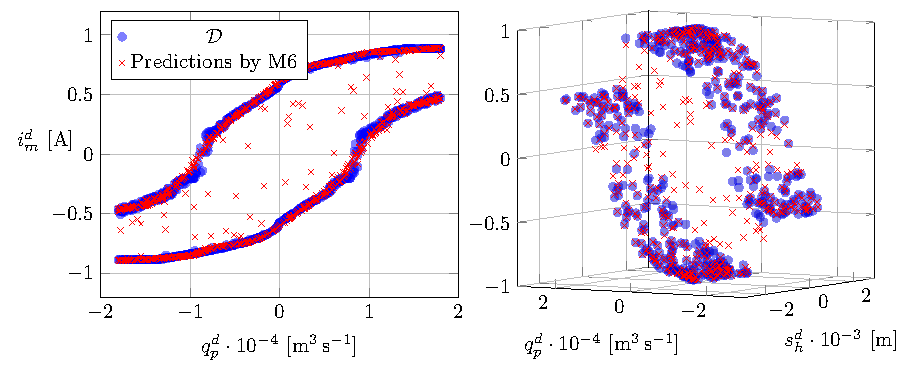
\includegraphics{graphics/pgfplots/cha5/Bosch/M6.pdf}
	\caption{Data $\mathcal{D}$ and predictions by model M6.}
	\label{fig:bosch-M6}
\end{figure}

To summarized, we see that the incorporation of a priori domain knowledge improves the quality of the fit for this example too. The constrained models show lower mean squared errors on the validation data as well as lower effective degrees of freedom. The superior model is clearly M6, since it has a significantly lower $\text{MSE}_{\text{val}}$ as well as EDoF. 
	\chapter{Boshc Data} \label{cha:real-world-application2}

As second example, we will now investigate the behavior of a servo-compensation, see~\pref{fig:blockschaltbild}. The region of interest is marked by the red square. We try to model the differential current $i_m^d$ by two inputs. The first input is the measured position of the main valve $s_h$. The second input is the differential flow $q_p^d$. 

\begin{figure}[H]
	\centering
	\includegraphics[width=0.8\columnwidth]{graphics/pgfplots/chaBosch/blockschaltbild.png}
	\caption{Blockschaltbild}
	\label{fig:blockschaltbild}
\end{figure}

The data is generated by using a validated model based on first-principles and is visualized in Figure \ref{fig:bosch_data_situation}. We know beforehand that the differential current $i_m^d$ is monotonic increasing with the differential flow $q_p^d$. 

\begin{figure}[H]
	\centering
	\includegraphics[width=0.8\columnwidth]{graphics/pgfplots/chaBosch/data_situation.png}
	\caption{Data Situation}
	\label{fig:bosch_data_situation}
\end{figure}

We will now again use various models based on B-spline bases, tensor-product B-spline bases and their shape-constraint alternatives to recover a model for the differential current. The following list, in which $s(i)$ denotes the use of a B-spline basis for input $i$ and $t(1,2)$ denotes the use of a tensor-product B-spline basis for inputs $i$ and $j$, describes the models.

\begin{enumerate}[(i)]
	\item M1 $= s(1) + s(2)$
	\item M2 $= s(1) + s(2)$, using monotonicity for $s(2)$
	\item M3 $= t(1,2)$
	\item M4 $= t(1,2)$, using monotonicity for input $s(1)$ and $s(2)$
	\item M5 $= s(2) + t(1,2)$, as additive model 
	\item M6 $= s(2) + t(1,2)$, as additive model using the constraints in M2 and M4
\end{enumerate}
%
To fit the models listed above, we perform a randomized train-validation split on the data, i.e. we split the data into a training set $\mathcal{D}_{\text{train}}$ and a validation set $\mathcal{D}_{\text{val}}$, fit the models to the resulting training set and evaluate its performance by calculating the mean squared error on the validation set $\mathcal{D}_{\text{val}}$ as well as by visual inspection.


Note that we use a smoothness penalty optimized via generalized cross-validation for each individual basis. The unconstraint models M1, M3 and M5 are therefore P-spline models rather than B-spline models. The shape-constraint models M2, M4 and M6 are SCP-spline models. 


\begin{comment}
content...
%
The mean squared errors evaluated on the validations set $\mathcal{D}_{\text{val}}$ are given in~\pref{tab:ebner-mse-val}. According to these, the best model is M4, i.e. the shape-constraint tensor-product B-spline with a monotonicity constraint in the mass flow dimension. The models M3, i.e. the tensor-product B-spline, and M6, i.e. the additive model using shape-constraints, perform nearly as well as M4 according to the mean squared error on the validation set. 

\begin{table}[H]
	\begin{center}
		\pgfplotstabletypeset[
		col sep=comma,
		columns/Model/.style={string type},
		columns/MSE_val/.style={column name={$\text{MSE}_{\text{val}}$}},
		every head row/.style={before row=\toprule[1pt] \toprule,after row=\midrule[2pt]},
		every last row/.style={after row=\bottomrule \bottomrule},
		every nth row={1}{before row=\midrule},
		]{graphics/data/cha5/mses.csv}
	\end{center}
	\caption{Mean squared errors on the validation set $\mathcal{D}_{\text{val}}$.}
	\label{tab:ebner-mse-val}
\end{table}

The predictions for model M4 are shown in~\pref{fig:ebner-M4}. The peak behavior in the temperature dimension is clearly visible, as well as an increasing trend within the massflow dimension. Therefore, we conclude that model M4 is the superior model with regards to the domain knowledge and data fidelity. 

\begin{figure}[H]
	\centering
	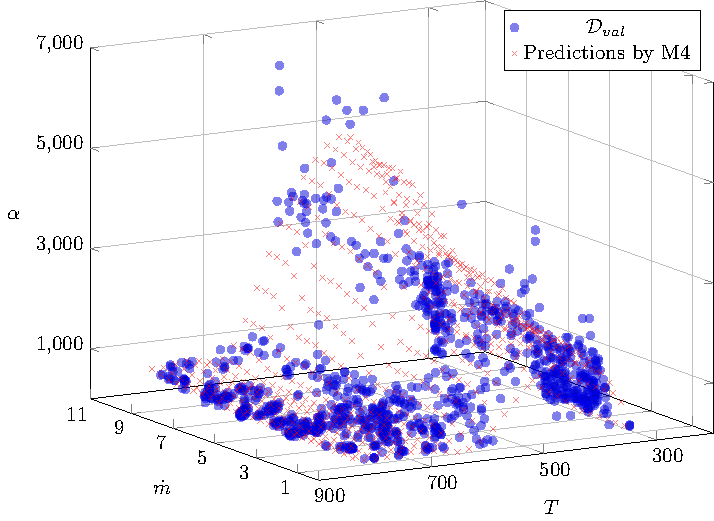
\includegraphics[width=\columnwidth]{graphics/pgfplots/cha5/M4.pdf}
	\caption{Validation set $\mathcal{D}_{\text{val}}$ and predictions by model M4.}
	\label{fig:ebner-M4}
\end{figure}

The predictions for model M6 are shown in~\pref{fig:ebner-M6}. Here, the peak behavior can also be identified, but in a weaker fashion as for model M4 in~\pref{fig:ebner-M4}. We also obtain an increasing trend in the massflow dimension. 

\begin{figure}[H]
	\centering
	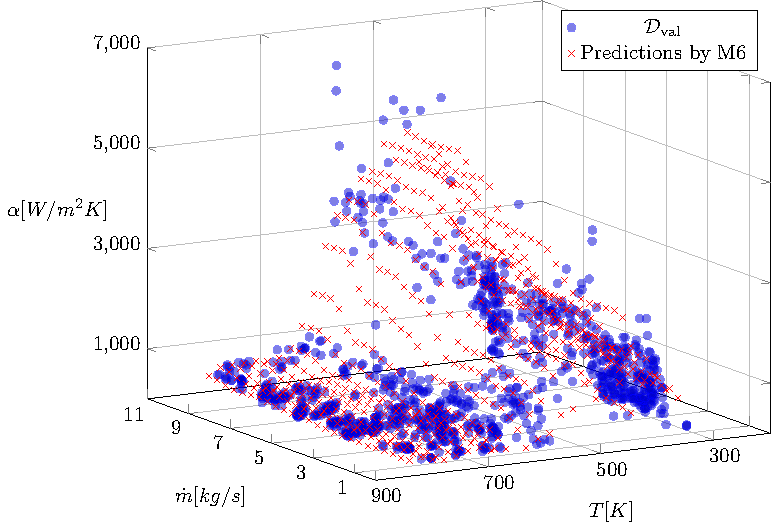
\includegraphics[width=\columnwidth]{graphics/pgfplots/cha5/M6.pdf}
	\caption{Validation set $\mathcal{D}_{\text{val}}$ and predictions by model M6.}
	\label{fig:ebner-M6}
\end{figure}
%
The visual inspection of the predictions of model M3 in~\pref{fig:ebner-M3} indicates that there is massive overfitting present. Neither smooth, nor the a priori known behavior (increasing in the massflow dimension and a peak behavior in the temperature dimension) is identifiable.  

\begin{figure}[H]
	\centering
	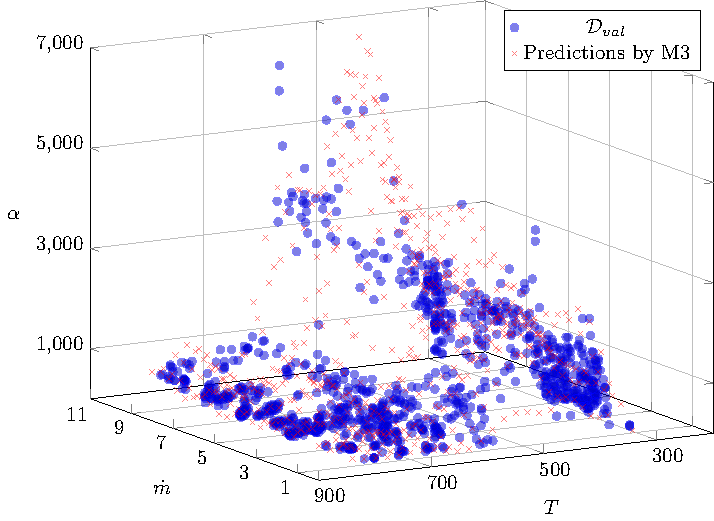
\includegraphics[width=\columnwidth]{graphics/pgfplots/cha5/M3.pdf}
	\caption{Validation set $\mathcal{D}_{\text{val}}$ and predictions by model M3.}
	\label{fig:ebner-M3}
\end{figure}

We omit the visual presentation of the predictions by the models M1, M2 and M5, since for all of these the mean squared errors on the validation set $\mathcal{D}_{\text{val}}$ is at least a magnitude higher, indicating even worse models.

To summarized, we see that the incorporation of a priori domain knowledge improves the quality of the fit in all of the above models, e.g. M2 is the better model according to the mean squared error on the validation set $\mathcal{D}_{\text{val}}$ than M1, M4 is better than M3 and M6 is better than M5. Therefore, we conclude that the use of a priori domain knowledge through shape-constraints improves the model quality for our real-world data example. 

\end{comment}

	%\chapter{Summary and Outlook} \label{cha:summary}

The main goal of this thesis was to find a way of including a priori domain knowledege into the fitting process of a data driven modeling approach. We showed that this is possible using the concept of shape constraints, see~\pref{cha:solution-approach}, and B-splines as well as additive regression for multi-dimensional data as presented in~\pref{cha:practical-considerations} and~\pref{cha:real-world-application}. Further, we presented an overview of the related literature regarding the topics of linear models, model selection and B-splines in~\pref{cha:fundamentals}. 

With regards to future work, it would be interesting to try to create an algorithm that automatically finds the best possible combination of univariate B-splines and tensor-product splines for some multi-dimensional problem with some a priori domain knowledge. For example, using 3 inputs, there are various combinations possible to create an additive model, e.g. a B-spline for dimension 1 and a tensor-product B-spline for dimension 2 and 3. An algorithm that automatically chooses the optimal combination with respect to some predefined criterion would help to enhance the usage of this approach.   
%	
	% Literaturverzeichnis...
	%=========================
	
	% falls ein Anhang vorhanden ist, hier einf�gen
	%\begin{appendices}
	
\chapter{Appendix} 
%%%%%%%%%%%%%%%%%%%%%%%%%%%%%%%%%%%%%%%%%%%%%%%%%%%%%%%%%%%%%%%%%%%%%%%%%%%%%%%%%%%
\section{Kronecker product} \label{apx:AppendixKronecker}

The Kronecker product $\vec{A} \otimes \vec{B}$ of the $n \times p$-matrix $\vec{A}$ and the $r \times q$-matrix $\vec{B}$ is defined as $nr \times pq$-matrix 

\begin{align}
	\vec{C} = \vec{A} \otimes \vec{B} = 
		\begin{bmatrix}
			a_{11} \vec{B} & \dots & a_{1p} \vec{B} \\
			\vdots 	       &       &  \vdots \\
			a_{n1} \vec{B} & \dots & a_{np} \vec{B}     
		\end{bmatrix}. 
\end{align}
%
As example, we define $\vec{A} \in \mathbb{R}^{3 \times 2}$ and $\vec{B} \in \mathbb{R}^{2 \times 2}$ as

\begin{align}
	\vec{A} = \begin{bmatrix}
			1 & 2  \\
			3 & 4 \\
			5 & 6		
		\end{bmatrix}, \quad 
	\vec{B} = 
		\begin{bmatrix}
			1 & 2  \\
			1 & 2   
		\end{bmatrix},
\end{align}
%
resulting in the matrix $\vec{C} \in \mathbb{R}^{6 \times 4}$ given by

\begin{align}
	\vec{C} = 
	\begin{bmatrix}
		a_{11} \vec{B} &  a_{12} \vec{B} \\
		a_{21} \vec{B} &  a_{22} \vec{B}
	\end{bmatrix} = 
	\begin{bmatrix}
		1 & 2 & 2 & 4  \\
		1 & 2 & 2 & 4 \\
		3 & 6 & 4 & 8 \\
		3 & 6 & 4 & 8 \\
		5 & 10& 6 &12 \\
		5 & 10& 6 &12
	\end{bmatrix}.
\end{align}

%%%%%%%%%%%%%%%%%%%%%%%%%%%%%%%%%%%%%%%%%%%%%%%%%%%%%%%%%%%%%%%%%%%%%%%%%%%%%%%%%%%
\section{Row-wise Kronecker product} \label{apx:AppendixKroneckerRowWise}

Given the $n \times p$-matrix$\vec{A}$ and the $n \times q$-matrix $\vec{B}$, the row-wise Kronecker product is defined as $n \times pq$-matrix $\vec{C}$ given by

\begin{align}
	\vec{C} = \vec{A} \odot \vec{B} = 
			\begin{bmatrix}
				a_{11} \vec{B}_1 & \dots & a_{1p} \vec{B}_1 \\
				\vdots 	   &         &  \vdots \\
				a_{n1} \vec{B}_n & \dots  & a_{np} \vec{B}_n     
			\end{bmatrix},
\end{align}
%
where $\vec{B}_i$ denotes the $i$-th row of the matrix $\vec{B}$. As example, we define $\vec{A} \in \mathbb{R}^{3 \times 3}$ and $\vec{B} \in \mathbb{R}^{3 \times 2}$ as

\begin{align}
	\vec{A} = 
		\begin{bmatrix}
			\vec{A}_1 \\
			\vec{A}_2 \\
			\vec{A}_3 
		\end{bmatrix} &= 
		\begin{bmatrix}
			1 & 2 & 3 \\
			4 & 5 & 6 \\
			7 & 8 & 9 
		\end{bmatrix}, \quad 
	\vec{B} = 
		\begin{bmatrix}
			\vec{B}_1 \\
			\vec{B}_2 \\
			\vec{B}_3 
		\end{bmatrix} = 
		\begin{bmatrix}
			1 & 2  \\
			1 & 2  \\
			1 & 2  
		\end{bmatrix},
\end{align}
%
resulting in the matrix $\vec{C} \in \mathbb{R}^{3 \times 6}$ given by

\begin{align}
		\vec{C} = 
	\begin{bmatrix}
		\vec{A}_1 \otimes \vec{B}_1 \\
		\vec{A}_2 \otimes \vec{B}_2 \\
		\vec{A}_3 \otimes \vec{B}_3 
	\end{bmatrix} = 
	\begin{bmatrix}
		1 & 2 & 2 & 4 & 3 & 6 \\
		4 & 8 & 5 &10 & 6 & 12\\
		7 & 14& 8 & 16& 9 & 19 
	\end{bmatrix}.
\end{align}
%
The row-wise Kronecker product is also known as \emph{face-splitting product} or as \emph{transposed Khatri-Rao product} \cite{slyusar1997analytical}.

%%%%%%%%%%%%%%%%%%%%%%%%%%%%%%%%%%%%%%%%%%%%%%%%%%%%%%%%%%%%%%%%%%%%%%%%%%%%%%%%%%%
\section{Derivation of the iterative scheme} \label{apx:AppendixB}

The following derivation is take from~\cite{bollaerts2006simple}. To find an optimal solution for the penalized least squares objective function for shape-constraint P-splines given by

\begin{align} \label{eq:L}
	\text{L}(\vec{\beta}) = \lVert \vec{y} - \vec{X} \vec{\beta} \rVert_2^2 + \lambda \transpose{\vec{\beta}} \vec{K} \vec{\beta} + \lambda_c \transpose{\vec{\beta}} \vec{K}_c \vec{\beta},
\end{align}
%
we use a Newton-Raphson scheme. At each iteration $i$, the new estimate $\hat{\vec{\beta}}_{i+1}$ is computed such that

\begin{align} \label{eq:NR-scheme}
	\vec{g}(\vec{\beta}_{i}) + \vec{H}(\vec{\beta}_{i}) \big( \vec{\beta}_{i+1} - \vec{\beta}_{i}\big) = 0,
\end{align}
%
with $\vec{g}$ being the gradient of and $\vec{H}$ being the Hessian of $\text{L}(\vec{\beta})$. The gradient of $\text{L}(\vec{\beta})$ equals to

\begin{align}
	\vec{g}(\vec{\beta}) = -2\transpose{\vec{X}} \vec{y} + 2\Big[ \transpose{\vec{X}} \vec{X} + \lambda \transpose{\vec{D}}_2 \vec{D}_2 + \lambda_c \transpose{\vec{D}}_c \vec{V}_c(\vec{\beta}) \vec{D}_c\Big] \vec{\beta} + \lambda_c \transpose{\vec{\beta}} \transpose{\vec{D}}_c \frac{\partial \vec{V}_c(\vec{\beta})}{\partial \vec{\beta}} \vec{D}_c \vec{\beta},
\end{align}
%
which can be simplified, see~\cite{bollaerts2006simple}, to

\begin{align} \label{eq:gradient-of-L}
	\vec{g}(\vec{\beta}) = -2\transpose{\vec{X}} \vec{y} + 2\Big[ \transpose{\vec{X}} \vec{X} + \lambda \transpose{\vec{D}}_2 \vec{D}_2 + \lambda_c \transpose{\vec{D}}_c \vec{V}_c(\vec{\beta}) \vec{D}_c\Big] \vec{\beta}. 
\end{align}
%
The gradient is therefore a piecewise linear function of $\vec{\beta}$ since $\vec{V}(\vec{\beta})$ is a diagonal matrix with 0s and 1s as diagonal elements, see~\pref{eq:gradient-of-L}. This implies that the Hessian is a step function of $\vec{\beta}$ and equal to

\begin{align} \label{eq:hessian-of-L}
	\vec{H}(\vec{\beta}) = 2\transpose{\vec{X}} \vec{X} + 2\lambda \transpose{\vec{D}}_2 \vec{D}_2 + 2\lambda_c \transpose{\vec{D}}_c \vec{V}_c(\vec{\beta}) \vec{D}_c + 2\lambda_c \transpose{\vec{D}}_c \frac{\partial \vec{V}_c(\vec{\beta})}{\partial \vec{\beta}} \vec{D}_c. 
\end{align}
%
The last part can be neglected again, see \cite{bollaerts2006simple}. Substituting~\pref{eq:gradient-of-L} and~\pref{eq:hessian-of-L} into~\pref{eq:NR-scheme} leads to

\begin{align}
	\begin{split}
	0 ={}& -2\transpose{\vec{X}} \vec{y} \\ 
	   {}&+ 2\Big[ \transpose{\vec{X}} \vec{X} + \lambda \transpose{\vec{D}}_2 \vec{D}_2 + \lambda_c \transpose{\vec{D}}_c \vec{V}_c(\vec{\beta}_i) \vec{D}_c\Big] \vec{\beta}_i \\ 
	   {}&+ 2\Big[\transpose{\vec{X}} \vec{X} + \lambda \transpose{\vec{D}}_2 \vec{D}_2 + \lambda_c \transpose{\vec{D}}_c \vec{V}_c(\vec{\beta}_i) \vec{D}_c \Big] \big( \vec{\beta}_{i+1} - \vec{\beta}_i \big),
	\end{split}
\end{align}
%
which can be reformulated as

\begin{align}
	-\transpose{\vec{X}} \vec{y} + \Big[ \transpose{\vec{X}} \vec{X} + \lambda \transpose{\vec{D}}_2 \vec{D}_2 + \lambda_c \transpose{\vec{D}}_c \vec{V}_c(\vec{\beta}_i) \vec{D}_c \Big] \vec{\beta}_{i+1} = 0,
\end{align}
%
and, hence, we obtain

\begin{align}
	\vec{\beta}_{i+1} = \Big[ \transpose{\vec{X}} \vec{X} + \lambda \transpose{\vec{D}}_2 \vec{D}_2 + \lambda_c \transpose{\vec{D}}_c \vec{V}_c(\vec{\beta}_i) \vec{D}_c \Big]^{-1} \transpose{\vec{X}} \vec{y}.
\end{align}

\end{appendices}
	
	%Literaturverzeichnis einfuegen
	\printbibliography

\end{document}
